\documentclass[fontset=fandol]{ctexrep}

\ctexset {
chapter = {
beforeskip = 0pt,
fixskip = true,
format = \Huge\bfseries,
nameformat = \rule{\linewidth}{1bp}\par\bigskip\hfill\chapternamebox,
number = \arabic{chapter},
aftername = \par\medskip,
aftertitle = \par\bigskip\nointerlineskip\rule{\linewidth}{2bp}\par
}
}
\newcommand\chapternamebox[1]{%
\parbox{\ccwd}{\linespread{1}\selectfont\centering #1}}
\xeCJKsetup{CJKmath=true}
\usepackage{amsmath}
\usepackage{amssymb}
\usepackage{amsthm}
\usepackage{xcolor}
\definecolor{bostonuniversityred}{rgb}{0.8, 0.0, 0.0}

\usepackage[shortlabels]{enumitem}
\setlist{nosep,left=\parindent}

\usepackage{graphicx}
\usepackage{wrapfig}
\usepackage{fancyhdr}
\usepackage{bm}
\usepackage{tasks}
\settasks{after-item-skip=0.5ex plus 0.5ex minus 1ex}
\NewTasksEnvironment[label={(\arabic*)}, item-indent=4em, label-offset=1em]{exer}[\item](2)
\usepackage{siunitx}
\usepackage{tocloft}
\tocloftpagestyle{empty}
\usepackage{etoolbox}
\patchcmd{\part}{plain}{empty}{}{}
\patchcmd{\chapter}{plain}{empty}{}{}
%\usepackage{showframe}%可以显示版面分布
\usepackage{tikz}
%\usepackage{draftwatermark}%设置水印
%\SetWatermarkAngle{30}
%\SetWatermarkScale{1.5}
%\SetWatermarkText{\textcolor{red!60}{\textit{ODE Solutions}}}
\usepackage{geometry}%设计版面格式
\geometry{inner=2cm,outer=3cm,marginparsep=2mm,marginparwidth=2.7cm}

\newcommand\diff{\,\mathrm{d}}
\newcommand\sgn{\,\mathrm{sgn}}
\newcommand\e{\mathrm{e}}
\newcommand\ii{\mathrm{i}}
\newcommand\bmitPhi{\bm{\varPhi}}
\newcommand\bmitPsi{\bm{\varPsi}}
\newcommand\T{\mathrm{T}}
\newcommand\rmJ{\mathrm{J}}
\renewcommand{\contentsname}{目录}

\makeatletter
\renewenvironment{proof}{\par
	\pushQED{\qed}%
	\normalfont \topsep1\p@\@plus6\p@\relax
	\trivlist
	\item\relax
	{\hspace*{\parindent}{\heiti 证明}\@addpunct{:}}\hspace\labelsep\ignorespaces
}{%
	\popQED\endtrivlist\@endpefalse
}
\makeatother
\makeatletter
\newenvironment{solve}{\par
	\pushQED{\qed}%
	\normalfont \topsep1\p@\@plus6\p@\relax
	\trivlist
	\item\relax
	{\hspace*{\parindent}{\heiti 解}\@addpunct{:}}\hspace\labelsep\ignorespaces
}{%
	\popQED\endtrivlist\@endpefalse
}
\makeatother
\usepackage[colorlinks=true,linkcolor=blue,unicode=true]{hyperref}

\begin{document}
\title{常微分方程教程习题解}
\author{SwitWu}
\maketitle

\tableofcontents
\cleardoublepage

\pagenumbering{arabic}
\setcounter{page}{1}
\chapter{基本概念}



\section{微分方程及其解的定义}



\begin{exercise}
  验证下列函数是右侧相应微分方程的解或通解:
  \begin{enumerate}[(1)]
  \item $y=C_1\e^{2x}+C_2\e^{-2x}:y''-4y=0$;
  \item $\displaystyle y=\frac{\sin x}{x}:xy'+y=\cos x$;
  \item $y=x\left(\int x^{-1}\e^x\diff x+C\right):xy'-y=x\e^x$;
  \item $y=\begin{cases}-\frac{1}{4}(x-C_1)^2,&-\infty<x<C_1,\\0,&C_1\leq x\leq C_2,\\+\frac{1}{4}(x-C_2)^2,&C_2<x<+\infty,\end{cases}:y'=\sqrt{|y|}$
  \end{enumerate}
\end{exercise}

\begin{proof}
  (1) $y=C_1\e^{2x}+C_2\e^{-2x}\Rightarrow y'=2C_1\e^{2x}-2C_2\e^{-2x}\Rightarrow y''=4C_1\e^{2x}+4C_2\e^{-2x}\Rightarrow y''-4y=0$;

  (2) $y=\frac{\sin x}{x}\Rightarrow y'=\frac{x\cos x-\sin x}{x^2}\Rightarrow xy'+y=\frac{x\cos x-\sin x}{x}+\frac{\sin x}{x}=\cos x$;

  (3) $y=x\left(\int x^{-1}\e^x\diff x+C\right)\Rightarrow y'=\int x^{-1}\e^x\diff x+C+\e^x\Rightarrow xy'-y=x(\int x^{-1}\e^x\diff x+C)+x\e^x-y=x\e^x$;

  (4) 当 $x<C_1$ 时, $y'=-\frac{1}{2}(x-C_1)$,
  而 $\sqrt{|y|}=\sqrt{\frac{1}{4}(x-C_1)^2}=\frac{1}{2}(C_1-x)$,
  故 $y'=\sqrt{|y|}(x<C_1)$, 其他两段同理可以验证.
\end{proof}



\begin{exercise}
  求下列初值问题的解:
  \begin{enumerate}[(1)]
  \item $y'''=x,y(0)=a_0,y'(0)=a_1,y''(0)=a_2;$
  \item $\frac{\diff y}{\diff x}=f(x),y(0)=0$ (这里 $f(x)$ 是一个连续函数);
  \item $\frac{\diff R}{\diff t}=-aR,R(0)=1$ (这里 $a>0$ 是一个常数);
  \item $\frac{\diff y}{\diff x}=1+y^2,y(x_0)=y_0.$
  \end{enumerate}
\end{exercise}

\begin{solve}
  (1) $y(x)=\frac{1}{24}x^4+\frac{a_2}{2}x^2+a_1x+a_0$;

  (2) $y(x)=\int_0^xf(t)\diff t$;

  (3) $R(t)=\e^{-at}$;

  (4) $y(x)=\tan(x+\arctan y_0-x_0)$.
\end{solve}



\begin{exercise}
  求出:
  \begin{enumerate}[(1)]
  \item 曲线族$y=Cx+x^2$所满足的微分方程;
  \item 曲线族$y=C_1\e^x+C_2x\e^x$所满足的微分方程;
  \item 平面上以原点为中心的一切圆所满足的微分方程;
  \item 平面上一切圆所满足的微分方程.
  \end{enumerate}
\end{exercise}

\begin{solve}
  (1) 求导得 $y'=C+2x$, 联立方程消去 $C$ 得 $y+x^2-xy'=0$.

  (2) 求两次导得
  $\begin{cases}y=C_1\e^x+C_2x\e^x\\y'=C_1\e^x+C_2(x+1)\e^x\\y''=C_1\e^x+C_2(x+2)\e^x\end{cases}$, 
  由前两个方程解得 $C_1=\frac{(x+1)y-xy'}{\e^x}$, $C_2=\frac{y'-y}{\e^x}$, 
  代入第三个方程得 $y''-2y'+y=0$.

  (3) 平面上以原点为中心的一切圆的参数方程为 $x^2+y^2=R^2$ ($R$ 为参数), 求导得 $x+yy'=0$.

  (4) 平面上一切圆的参数方程为 $(x-a)^2+(y-b)^2=R^2$ ($a,b,R$ 为参数)
  关于 $x$ 求三次导并消去参数即得 $3y'(y'')^2-\bigl[1+(y')^2\bigr]y'''=0$.
\end{solve}



\begin{exercise}
证明: 设 $y=g(x,C_1,C_2,\cdots,C_n)$ 是一个充分光滑的函数族, 其中 $x$ 是自变量, 
而 $C_1, C_2, \cdots, C_n$ 是 $n$ 个独立的参数(任意常数), 则存在一个形如 (1.1) 的 $n$ 阶微分方程, 
使得它的通解恰好是上述函数族.
\end{exercise}

\begin{proof}
  已知
  \begin{equation}
    \begin{cases}
    y=g(x,C_1,C_2,\cdots,C_n)\\
    y'=g^{(1)}(x,C_1,C_2,\cdots,C_n)\\\cdots\\
    y^{(n-1)}=g^{(n-1)}(x,C_1,C_2,\cdots,C_n)\\
    y^{(n)}=g^{(n)}(x,C_1,C_2,\cdots,C_n)
    \end{cases}\tag{$\star$}
  \end{equation}
  因为 $C_1,C_2,\cdots,C_n$ 独立, 所以 Jacobi 行列式
  \[\frac{D[g,g^{(1)},\cdots,g^{(n-1)}]}{D[C_1,C_2,\cdots,C_n]}=\begin{vmatrix}
  \frac{\partial g}{\partial C_1}&\frac{\partial g}{\partial C_2}&\cdots&\frac{\partial g}{\partial C_n}
  \\
  \frac{\partial g^{(1)}}{\partial C_1}&\frac{\partial g^{(1)}}{\partial C_2}&\cdots&\frac{\partial g^{(1)}}{\partial C_n}\\
  \vdots&\vdots&&\vdots\\
  \frac{\partial g^{(n-1)}}{\partial C_1}&\frac{\partial g^{(n-1)}}{\partial C_2}&\cdots&\frac{\partial g^{(n-1)}}{\partial C_n}\end{vmatrix}\neq 0.\]
  由隐函数存在定理知可由方程组 $(\star)$ 的前 $n$ 个方程解出
  \[C_i=C_i(x,y,\cdots,y^{(n-1)})(i=1,2,\cdots,n).\]
  将之代入方程组 $(\star)$ 最后一个方程中得
  \[y^{(n)}=g^{(n)}(x,C_1(x,y,\cdots,y^{(n-1)}),\cdots,C_n(x,y,\cdots,y^{(n-1)})).\]
  上式即为所求的 $n$ 阶微分方程.
\end{proof}



\section{微分方程及其解的几何解释}



\begin{exercise}
  作出如下微分方程的线素场:
  \begin{enumerate}[(1)]
  \item $\displaystyle y'=\frac{xy}{|xy|}$;
  \item $y'=(y-1)^2$;
  \item $y'=x^2+y^2$.
  \end{enumerate}
\end{exercise}

\begin{solve}
  (1)奇异点集合为 $\{(x,y)\mid x=0\text{\ 或\ }y=0\}$, 线素场如图 (Matlab 制图).
  \begin{figure}[htb]
  \centering
  \includegraphics[width=4cm]{figure/ODE1_2_1.png}
  \caption{(1)题图}
  \end{figure}

  (2)等斜线为$(y-1)^2=k\Rightarrow y=1\pm\sqrt{k}$, 线素场如图.
  \begin{figure}[htb]
  \centering
  \includegraphics[width=4cm]{figure/ODE1_2_2.png}
  \caption{(2)题图}
  \end{figure}

  (3)等斜线为$x^2+y^2=k$, 线素场如图.
  \begin{figure}[htb]
  \centering
  \includegraphics[width=4cm]{figure/ODE1_2_3.png}
  \caption{(3)题图}
  \end{figure}
\end{solve}



\begin{exercise}
  利用线素场研究下列微分方程的积分曲线族:
  \begin{enumerate}[(1)]
    \item $y' = 1+xy$;
    \item $y' = x^2-y^2$.
  \end{enumerate}
\end{exercise}



\begin{exercise}
  根据磁场的物理直观, 试作微分方程 (2.8) 的线素场及其积分曲线族的草图.
\end{exercise}
\chapter{初等积分法}



\section{恰当方程}



\begin{exercise}
  判断下列方程是否为恰当方程; 并且对恰当方程求解.
  \begin{enumerate}[(1)]
  \item $(3x^2-1)\diff x+(2x+1)\diff y=0$.
  \item $(x+2y)\diff x+(2x-y)\diff y=0$.
  \item $(ax+by)\diff x+(bx+cy)\diff y=0$.
  \item $(ax-by)\diff x+(bx-cy)\diff y=0(b\neq0)$.
  \item $(t^2+1)\cos u\diff u+2t\sin u\diff t=0$.
  \item $(y\e^x+2\e^x+y^2)\diff x+(\e^x+2xy)\diff y=0$.
  \item $\displaystyle\left(\frac{y}{x}+x^2\right)\diff x+(\ln x-2y)\diff y=0$.
  \item $(ax^2+by^2)\diff x+cxy\diff y=0$.
  \item $\displaystyle\frac{2s-1}{t}\diff s+\frac{s-s^2}{t^2}\diff t=0$.
  \item $xf(x^2+y^2)\diff x+yf(x^2+y^2)\diff y=0$, 其中$f(\cdot)$是连续可微的.
  \end{enumerate}
\end{exercise}

\begin{solution}
	\begin{enumerate}[(1)]
		\item $\frac{\partial P}{\partial y}=0,\frac{\partial Q}{\partial x}=2$, 不是恰当方程.
		\item $\frac{\partial P}{\partial y}=2,\frac{\partial Q}{\partial x}=2$, 是恰当方程, 因为
			  \[(x+2y)\diff x+(2x-y)\diff y=\diff\left(\frac{1}{2}x^2+2xy-\frac{1}{2}y^2\right),\]
			  所以通积分为
			  \[\frac{1}{2}x^2+2xy-\frac{1}{2}y^2=C.\]
		\item $\frac{\partial P}{\partial y}=b=\frac{\partial Q}{\partial x}$, 是恰当方程, 因为
			  \[(ax+by)\diff x+(bx+cy)\diff y=\diff\left(\frac{1}{2}ax^2+bxy+\frac{1}{2}cy^2\right),\]
			  所以通积分为
			  \[\frac{1}{2}ax^2+bxy+\frac{1}{2}cy^2 = C.\]
		\item $\frac{\partial P}{\partial y}=-b\neq\frac{\partial Q}{\partial x}=b$, 不是恰当方程.
		\item $\frac{\partial P}{\partial t}=2t\cos u=\frac{\partial Q}{\partial u}$, 故是恰当方程, 因为
			  \[(t^2+1)\cos u\diff u+2t\sin u\diff t=\diff\left((t^2+1)\sin u\right),\]
			  所以通积分为
			  \[(t^2+1)\sin u = C.\]
		\item $\frac{\partial P}{\partial y}=\e^x+2y=\frac{\partial Q}{\partial x}$, 是恰当方程, 因为
			  \[(y\e^x+2\e^x+y^2)\diff x+(\e^x+2xy)\diff y=\diff(y\e^x+xy^2+2\e^x),\]
			  所以通积分为
			  \[y\e^x+xy^2+2\e^x = C.\]
		\item $\frac{\partial P}{\partial y}=\frac{1}{x}=\frac{\partial Q}{\partial x}$, 是恰当方程, 因为
			  \[\left(\frac{y}{x}+x^2\right)\diff x+(\ln x-2y)\diff y=\diff\left(y\ln x+\frac{1}{3}x^3-y^2\right),\]
			  所以通积分为
			  \[y\ln x+\frac{1}{3}x^3-y^2=C.\]
		\item $\frac{\partial P}{\partial y}=2by,\frac{\partial Q}{\partial x}=cy$, 
      因此当$2b=c$时方程为恰当方程, 此时
      \[(ax^2+by^2)\diff x+cxy\diff y=(ax^2+by^2)\diff x+2bxy\diff y
        = \diff\left(\frac{1}{3}ax^3+bxy^2\right),\]
      所以通积分为
      \[\frac{1}{3}ax^3+bxy^2 = C.\]
      当 $2b\neq c$ 时, 方程不是恰当方程.
		\item $\frac{\partial P}{\partial t}=\frac{1-2s}{t^2}=\frac{\partial Q}{\partial s}$, 
      是恰当方程, 因为
      \[\frac{2s-1}{t}\diff s+\frac{s-s^2}{t^2}\diff t=\diff\left(\frac{s^2-s}{t}\right),\]
      所以通积分为
      \[\frac{s^2-s}{t}=C.\]
		\item $\frac{\partial P}{\partial y}=2xyf'(x^2+y^2)=\frac{\partial Q}{\partial x}$, 
      是恰当方程, 且通积分为
			\[F(x^2+y^2)=C,\text{其中\ }F\text{\ 是\ }f\text{\ 的不定积分}.\qedhere\]
	\end{enumerate}
\end{solution}



\section{变量分离的方程}



\begin{exercise}
  求解下列微分方程, 并指出这些方程在$Oxy$平面上有意义的区域:
  \begin{enumerate}[(1)]
  \item $\displaystyle\frac{\diff y}{\diff x}=\frac{x^2}{y}$;
  \item $\displaystyle\frac{\diff y}{\diff x}=\frac{x^2}{y(1+x^3)}$;
  \item $\displaystyle\frac{\diff y}{\diff x}+y^2\sin x=0$;
  \item $\displaystyle\frac{\diff y}{\diff x}=1+x+y^2+xy^2$;
  \item $\displaystyle\frac{\diff y}{\diff x}=(\cos x\cos 2y)^2$;
  \item $\displaystyle x\frac{\diff y}{\diff x}=\sqrt{1-y^2}$;
  \item $\displaystyle\frac{\diff y}{\diff x}=\frac{x-\e^x}{y+\e^y}$.
  \end{enumerate}
\end{exercise}

\begin{solution}
  (1) $y^2=\frac{2}{3}x^3+C,y\neq 0$;

  (2) $y^2=\frac{2}{3}\ln|1+x^3|+C,y\neq0,x\neq-1$;

  (3) $\frac{1}{y}+\cos x=C$, 特解: $y=0$;

  (4) $y=\tan(x+\frac{1}{2}x^2+C)$;

  (5) 当 $\cos 2y\neq 0$ 时, 原方程等价于 $\frac{\diff y}{\cos^2 2y}=\sec^2 2y\diff y=\cos^2x\diff x$, 
  积分得 $2x+\sin2x-2\tan2y=C$, 当 $\cos2y=0$时, 有特解 $y=\frac{\pi}{4}+\frac{k\pi}{2}(k\in\mathbb{Z})$;

  (6) $\arcsin y=\ln|x|+C$, 特解: $y=\pm 1$;

  (7) $y^2-x^2+2(\e^y-\e^{-x})=C$ $(y+\e^y\neq 0)$.
\end{solution}



\begin{exercise}
  求解下列微分方程的初值问题:
  \begin{enumerate}[(1)]
  \item $\displaystyle\sin 2x\diff x+\cos 3y\diff y=0,\quad y\left(\frac{\pi}{2}\right)=\frac{\pi}{3}$;
  \item $\displaystyle x\diff x+y\e^{-x}\diff y=0,\quad y(0)=1$;
  \item $\displaystyle\frac{\diff r}{\diff\theta}=r,\quad r(0)=2$;
  \item $\displaystyle\frac{\diff y}{\diff x}=\frac{\ln|x|}{1+y^2},\quad y(1)=0$;
  \item $\displaystyle\sqrt{1+x^2}\frac{\diff y}{\diff x}=xy^3,\quad y(0)=1$.
  \end{enumerate}
\end{exercise}

\begin{solution}
  (1) 积分得 $-\frac{1}{2}\cos2x+\frac{1}{3}\sin3y+C=0$, 
  由 $y\left(\frac{\pi}{2}\right)=\frac{\pi}{3}$ 得 $C=-\frac{1}{2}$,
  因此原方程的解为 $2\sin3y-3\cos2x-3=0$.

  (2) 原方程等价于 $x\e^x\diff x+y\diff y=0$, 积分得 $(x-1)\e^x+\frac{1}{2}y^2+C=0$, 
  代入初值条件 $y(0)=1$ 得 $C=\frac{1}{2}$, 因此原方程的解为 $2(x-1)\e^x+y^2+1=0$.

  (3) 由初值条件知 $r\neq0$, 故 $\frac{\diff r}{r}=\diff\theta$, 积分得 $r=C\e^{\theta}$ $(C\neq 0)$,
  代入初值条件得 $C=2$, 因此原方程的解为 $r=2\e^{\theta}$.

  (4) $(1+y^2)\diff y=\ln|x|\diff x$, 积分得 $y+\frac{1}{3}y^3=x(\ln|x|-1)+C$, 
  代入初值条件得$C=1$, 因此原方程的解为 $y+\frac{1}{3}y^3=x(\ln|x|-1)+1$.

  (5) 由初值条件知 $y\neq 0$, 故原方程等价于 $\frac{\diff y}{y^3}=\frac{x}{\sqrt{1+x^2}}\diff x$, 
  积分得 $-\frac{1}{2}y^{-2}=\sqrt{1+x^2}+C$, 代入初值条件得 $C=-\frac{3}{2}$, 
  因此原方程的解为 $2\sqrt{1+x^2}+y^{-2}-3=0$.
\end{solution}



\begin{exercise}
  求解下列微分方程, 并作出相应积分曲线族的简图:
  \begin{enumerate}[(1)]
  \item $\displaystyle\frac{\diff y}{\diff x}=\cos x$;
  \item $\displaystyle\frac{\diff y}{\diff x}=ay$ $(a\neq 0\text{\ 为常数})$;
  \item $\displaystyle\frac{\diff y}{\diff x}=1-y^2$;
  \item $\displaystyle\frac{\diff y}{\diff x}=y^n$ $(n=\frac{1}{3},1,2)$.
  \end{enumerate}
\end{exercise}

\begin{solution}
  (1) $y=\sin x+C$, 积分曲线族如图~\ref{fig2.1}.
  \begin{figure}[htb]
    \centering
    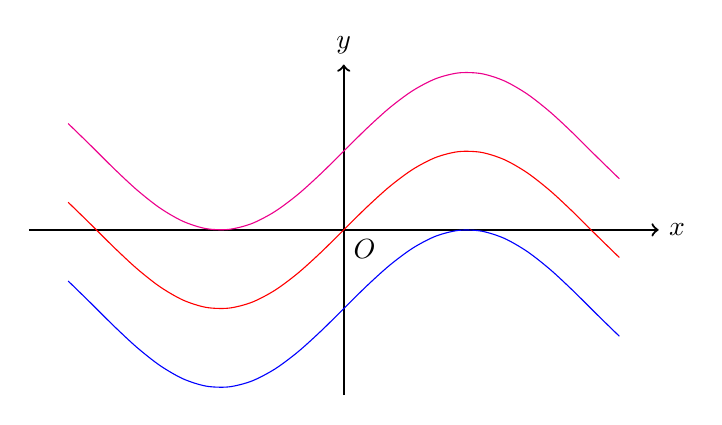
\begin{tikzpicture}[domain=-3.5:3.5]
    \draw[->,thick] (-4,0)--(4,0)node[anchor=west]{$x$};
    \draw[->,thick] (0,-2.1)--(0,2.1)node[anchor=south]{$y$};
    \draw (0,0)node[anchor=north west]{$O$};
    \draw[color=red,smooth] plot(\x,{sin(\x r)});
    \draw[color=blue,smooth]plot(\x,{sin(\x r)-1});
    \draw[color=magenta,smooth]plot(\x,{sin(\x r)+1});
    \end{tikzpicture}
    \caption{$y=\sin x+C$}
    \label{fig2.1}
  \end{figure}

  (2) $y=0$为特解, 当 $y\neq 0$ 时, 积分得$y=C\e^{ax}$ $(C\neq 0)$, 
  积分曲线族如图~\ref{fig2.2} (以 $a>0$ 为例).
  \begin{figure}
    \centering
    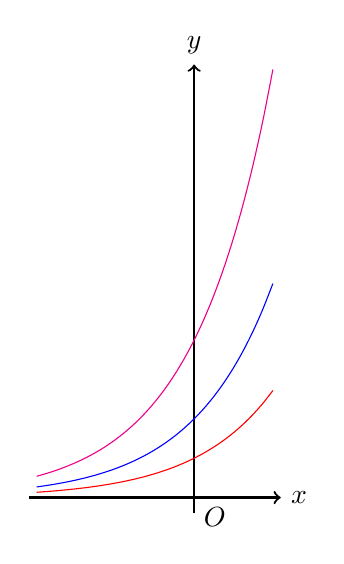
\begin{tikzpicture}[domain=-2:1]
    \draw[->,thick] (-2.1,0)--(1.1,0)node[anchor=west]{$x$};
    \draw[->,thick] (0,-0.2)--(0,5.5)node[anchor=south]{$y$};
    \draw (0,0)node[anchor=north west]{$O$};
    \draw[color=red,smooth]plot(\x,{0.5*exp(\x)});
    \draw[color=blue,smooth]plot(\x,{exp(\x)});
    \draw[color=magenta,smooth]plot(\x,{2*exp(\x)});
    \end{tikzpicture}
    \caption{$y=C\e^{ax}$}
    \label{fig2.2}
  \end{figure}

  (3) $y=\pm1$为特解, 当 $y\neq\pm 1$ 时, $\frac{\diff y}{1-y^2}=\diff x$, 
  积分得 $y=\frac{C\e^{2x}-1}{C\e^{2x}+1}(C\neq0)$, 
  当$C>0$时, 函数图像位于直线 $y=1$ 和 $y=-1$ 之间且单调递增; 
  当$C<0$时, 存在间断点 $x_0=\frac{1}{2}\ln\left(-\frac{1}{C}\right)$, 
  $y=y(x)$ 在 $(-\infty,x_0)$ 上单调递减且当 $x\to x_0-$ 时 $y\to-\infty$, 
  在 $(x_0,\infty)$ 上单调递减且当 $x\to x_0+$ 时 $y\to+\infty$, 积分曲线族如图~\ref{fig2.3}.
  \begin{figure}
    \centering
    \begin{tikzpicture}[domain=-3.5:3.5]
      \draw[->,thick] (-4,0)--(4,0)node[anchor=west]{$x$};
      \draw[->,thick] (0,-5)--(0,6)node[anchor=south]{$y$};
      \draw(0,0)node[anchor=south east]{$O$};
      \draw[color=yellow,smooth]plot(\x,1);
      \draw[color=yellow,smooth]plot(\x,-1);
      \draw(-2,1)node[anchor=south]{$y=1$};
      \draw(2,-1)node[anchor=south]{$y=-1$};
      \draw[dashed](0.3466,-5)--(0.3466,6);
      \draw(0.3466,-2)node[anchor=west]{$x=\frac{1}{2}\ln\left(-\frac{1}{C}\right)(C<0)$};
      \draw[color=red,smooth]plot(\x,{(exp(2*\x)-1)/(exp(2*\x)+1)});
      \draw[color=red,smooth]plot(\x,{(2*exp(2*\x)-1)/(2*exp(2*\x)+1)});
      \draw[color=red,smooth]plot(\x,{(0.5*exp(2*\x)-1)/(0.5*exp(2*\x)+1)});
      \draw[color=red,smooth]plot(\x,{(exp(2*\x)-1)/(exp(2*\x)+1)});
      \draw[color=blue,smooth,domain=-3.5:0.15]plot(\x,{(-0.5*exp(2*\x)-1)/(-0.5*exp(2*\x)+1)});
      \draw[color=blue,smooth,domain=0.55:3.5]plot(\x,{(-0.5*exp(2*\x)-1)/(-0.5*exp(2*\x)+1)});
    \end{tikzpicture}
  \caption{$y=\pm 1$和$y=\frac{C\e^{2x}-1}{C\e^{2x}+1}$}
  \label{fig2.3}
  \end{figure}

  (4) 下述三种情形积分曲线族都易作出(略去).
  \begin{enumerate}[(i)]
  \item $n=\frac{1}{3}$ 时, 通解为 $\frac{3}{2}y^{\frac{2}{3}}=x+C$ $(x\geq-C)$, 特解为 $y=0$;
  \item $n=1$时, 通解为 $y=C\e^x$ $(C\in\mathbb{R})$;
  \item $n=2$时, 通解为 $y=\frac{1}{-x+C}$ $(C\in\mathbb{R})$, 特解为$y=0$.
  \end{enumerate}
\end{solution}



\begin{exercise}
  跟踪: 设某 $A$ 从 $Oxy$ 平面上的原点出发, 沿 $x$ 轴正方向前进; 同时某 $B$ 从点 $(0,b)$ 开始跟踪 $A$, 
  即 $B$ 的运动方向永远指向 $A$ 并与 $A$ 保持等距 $b$. 试求 $B$ 的光滑运动轨迹.
\end{exercise}

\begin{solution}
  设 $B$ 的运动轨迹方程为 $y=y(x)$, 记某时刻 $B$ 的位置为 $(x,y(x))$, 
  则此时 $A$ 相应的位置为 $\left(x-\frac{y(x)}{y'(x)},0\right)$, 由于 $A$ 与 $B$ 保持等距, 故
  \[\left(\frac{y}{y'}\right)^2+y^2=b^2\Rightarrow\diff x=-\frac{\sqrt{b^2-y^2}}{y}\diff y.\]
  积分得
  \[\begin{split}
  x
  & = -\int\frac{\sqrt{b^2-y^2}}{y}\diff y(y=b\cos\theta) \\
  & = -\int\frac{b\sin\theta}{b\cos\theta}(-b\sin\theta)\diff\theta \\
  & = b\int(\sec\theta-\cos\theta)\diff\theta \\
  & = b\ln|\sec\theta+\tan\theta|-b\sin\theta+C \\
  & = b\ln\frac{b+\sqrt{b^2-y^2}}{y}-\sqrt{b^2-y^2}+C.
  \end{split}\]
  由初值条件 $y(0)=b$ 得 $C=0$, 故 $B$ 的光滑运动轨迹方程为
  $x=b\ln\frac{b+\sqrt{b^2-y^2}}{y}-\sqrt{b^2-y^2}$.
\end{solution}



\begin{exercise}
  设微分方程
  \[\frac{\diff y}{\diff x}=f(y),\]
  其中 $f(y)$ 在 $y=a$ 的某邻域 (例如区间 $|y-a|\leq\varepsilon$) 内连续, 而且$f(y)=0$当且仅当$y=a$. 
  证明: 在直线$y=a$上的每一点, 上述方程的解是局部唯一的, 当且仅当瑕积分
  \[\left|\int_a^{a\pm\varepsilon}\frac{\diff y}{f(y)}\right|=\infty.\]
\end{exercise}

\begin{solution}
  ($\Leftarrow$) 显然, $y=a$ 是方程的一个解, 用反证法, 设 $y=y(x)$ 是方程的另一个解, 
  它与直线 $y=a$ 相交. 不妨设 $(x_0,a)$ 是它们的一个交点, 
  且存在区间 $I=(x_0,x_0+\delta)$ 或 $I=(x_0-\delta,x_0)$, 
  使得当 $x\in I$ 时, $y(x)\neq a$, 从而
  \[\frac{\diff y(x)}{f(y(x))}=\diff x,\quad x\in I.\]
  积分得
  \[\int_a^y\frac{\diff y}{f(y)}=\int_{x_0}^x\frac{\diff y(x)}{f(y(x))}
    = \int_{x_0}^x\diff x = x-x_0<\infty.\]
  矛盾.

  $(\Rightarrow)$ 用反证法, 设 $\left|\int_a^{a\pm\varepsilon}\frac{\diff y}{f(y)}\right|<+\infty$,
  则由
  \[\int_a^y\frac{\diff y}{f(y)}=x-x_0\]
  定义的函数是方程的解, 且通过点 $(x_0,a)$, 而 $y=a$ 也是过点 $(x_0,a)$ 的解, 矛盾.
\end{solution}



\begin{exercise}
  利用上题结果,作出下列微分方程积分曲线族的草图:
  \[(1)\frac{\diff y}{\diff x}=\sqrt{|y|};\quad
  (2)\frac{\diff y}{\diff x}=
  \begin{cases}
    y\ln|y|, & y\neq 0, \\
    0,       & y=0.
  \end{cases}\]
\end{exercise}

\begin{solution}
(1) 因为 $\int_0^{\pm\varepsilon}\frac{\diff y}{\sqrt{|y|}}$ 收敛, 故解不是局部唯一的, 微分方程的通解为
\[y=
  \begin{cases}
    \frac{1}{4}(x+C)^2,  & x\geq -C, \\
    -\frac{1}{4}(x+C)^2, & x\leq -C.
  \end{cases}\]
另外特解为 $y=0$, 积分曲线族容易作出.

(2) 因为 $\int_0^{\pm\varepsilon}\frac{\diff y}{y\ln|y|}$ 发散, 所以解是局部唯一的, 微分方程的通解为
\[y=\pm\e^{C\e^x}\quad(C\in\mathbb{R}).\]
另外特解为 $y=0$, 积分曲线族容易作出.
\end{solution}



\section{一阶线性方程}



\begin{exercise}
  求解微分方程:
  \begin{enumerate}[(1)]
  \item $\displaystyle\frac{\diff y}{\diff x}+2y=x\e^{-x}$;
  \item $\displaystyle\frac{\diff y}{\diff x}+y\tan x=\sin(2x)$;
  \item $\displaystyle x\frac{\diff y}{\diff x}+2y=\sin x$, $y(\pi)=\frac{1}{\pi}$;
  \item $\displaystyle\frac{\diff y}{\diff x}-\frac{1}{1-x^2}y=1+x$, $y(0)=1$.
  \end{enumerate}
\end{exercise}

\begin{solution}
  (1) $p(x)=2$, $q(x)=x\e^{-x}$, 故
  \[y=\e^{-\int2\diff x}\left(C+\int x\e^{-x}\e^{\int2\diff x}\diff x\right)=C\e^{-2x}+(x-1)\e^{-x}.\]

  (2) $p(x)=\tan x$, $q(x)=\sin(2x)$, 故
  \[\begin{split}
  y
  & = \e^{-\int\tan x\diff x}\left(C+\int\sin(2x)\e^{\int\tan x\diff x}\diff x\right)\\
  & = |\cos x|\left(C+\int\frac{\sin(2x)}{|\cos x|}\diff x\right)=C|\cos x|-2\cos^2x。
  \end{split}\]

  (3) $p(x)=\frac{2}{x}$, $q(x)=\frac{\sin x}{x}$, 故
  \[y=\e^{-\int\frac{2}{x}\diff x}\left(C+\int\frac{\sin x}{x}\e^{\int\frac{2}{x}\diff x}\diff x\right)=\frac{1}{x^2}(C+\sin x-x\cos x).\]
  代入初值条件得 $C=0$, 故原方程的解为
  \[y=\frac{\sin x}{x^2}-\frac{\cos x}{x}.\]

  (4) $p(x) = -\frac{1}{1-x^2}$, $q(x)=1+x$, 故
  \begin{align*}
    y
    & = \e^{\int\frac{1}{1-x^2}\diff x}\left(C+\int(1+x)\e^{\int\frac{1}{x^2-1}\diff x}\diff x\right) \\
    & = \left|\frac{x+1}{x-1}\right|^{\frac{1}{2}}\left(C+\int(1+x)\left|\frac{x-1}{x+1}\right|^{\frac{1}{2}}\diff x\right)\\
    & = \begin{cases}
      \sqrt{\frac{x+1}{x-1}}\left(C+\int\sqrt{x^2-1}\diff x\right), & |x|>1, \\
      \sqrt{\frac{x+1}{1-x}}\left(C+\int\sqrt{1-x^2}\diff x\right), & |x|<1,
    \end{cases} \\
    & = \begin{cases}
      \sqrt{\frac{x+1}{x-1}}\left(C+\frac{1}{2}x\sqrt{x^2-1}-\frac{1}{2}\ln|x+\sqrt{x^2-1}|\right),
        & |x|>1, \\
        \sqrt{\frac{x+1}{1-x}}\left(C+\frac{1}{2}\arcsin x+\frac{1}{2}x\sqrt{1-x^2}\right),
        & |x|<1.
    \end{cases}\qedhere
  \end{align*}
\end{solution}



\begin{exercise}
  把下列微分方程化为线性微分方程:
  \begin{enumerate}[(1)]
  \item $\displaystyle\frac{\diff y}{\diff x}=\frac{x^2+y^2}{2y}$;
  \item $\displaystyle\frac{\diff y}{\diff x}=\frac{y}{x+y^2}$;
  \item $\displaystyle 3xy^2\frac{\diff y}{\diff x}+y^3+x^3=0$;
  \item $\displaystyle\frac{\diff y}{\diff x}=\frac{1}{\cos y}+x\tan y$.
  \end{enumerate}
\end{exercise}

\begin{solution}
  (1) 令 $u=y^2$, 则 $\frac{\diff u}{\diff x}=2y\frac{\diff y}{\diff x}=x^2+u$.

  (2) 将 $x$ 看作 $y$ 的函数, 即 $\frac{\diff x}{\diff y}=\frac{x}{y}+y$.

  (3) 令 $u=y^3$, 则 $\frac{\diff u}{\diff x}=3y^2\frac{\diff y}{\diff x}=-\frac{u}{x}-x^2$.

  (4) 原方程变形为 $\cos y\frac{\diff y}{\diff x}=1+x\sin y$,
  令 $u=\sin y$, 即得 $\frac{\diff u}{\diff x}=1+xu$.
\end{solution}



\begin{exercise}
  设 $y=\varphi(x)$ 满足微分不等式
  \[y'+a(x)y\leq 0\quad (x\geq 0).\]
  求证:
  \[\varphi(x)\leq\varphi(0)\e^{-\int_0^x a(s)\diff s}\quad (x\geq 0).\]
\end{exercise}

\begin{proof} 
在不等式两边同时乘以 $\e^{\int_0^xa(s)\diff s}$, 得
\[\e^{\int_0^xa(s)\diff s}\frac{\diff y}{\diff x}+a(x)y\e^{\int_0^xa(s)\diff s}\leq 0,\]
即
\[\frac{\diff\left(\varphi(x)\e^{\int_0^xa(s)\diff s}\right)}{\diff x}\leq 0.\]
将上式从 $0$ 到 $x$ 积分得
\[\varphi(x)\e^{\int_0^xa(s)\diff s}-\varphi(0)\leq 0
\Rightarrow\varphi(x)\leq\varphi(0)\e^{-\int_0^xa(s)\diff s}.\qedhere\]
\end{proof}



\begin{exercise}
  用常数变易法求解非齐次线性方程 $\frac{\diff y}{\diff x}+p(x)y=q(x)$, 即: 
  假设方程有形如 $y=C\e^{-\int p(x)\diff x}$ 的解, 但其中的常数 $C$ 变易为 $x$ 的一个待定函数 $C(x)$. 
  然后将这种形式的解代入原方程, 再去确定 $C(x)$.
\end{exercise}

\begin{solution}
因为
\[y=C(x)\e^{-\int p(x)\diff x},\]
所以
\[\frac{\diff y}{\diff x}=C'(x)\e^{-\int p(x)\diff x}+C(x)(-p(x))\e^{-\int p(x)\diff x}.\]
即
\[\frac{\diff y}{\diff x}+p(x)y=C'(x)\e^{-\int p(x)\diff x}.\]
故有
\[C'(x)\e^{-\int p(x)\diff x} = q(x).\]
解之得
\[C(x)=\int q(x)\e^{\int p(x)\diff x}\diff x+C.\]
代回即得原方程的解为
\[y=\e^{-\int p(x)\diff x}\left(C+\int q(x)\e^{\int p(x)\diff x}\diff x\right).\qedhere\]
\end{solution}



\begin{exercise}
  考虑方程
  \[\frac{\diff y}{\diff x}+p(x)y=q(x),\]
  其中 $p(x)$ 和 $q(x)$ 都是以 $\omega>0$ 为周期的连续函数. 试证:

  (1) 若 $q(x)\equiv 0$, 则方程的任一非零解以 $\omega$ 为周期, 当且仅当函数 $p(x)$ 的平均值
  \[\bar{p}=\frac{1}{\omega}\int_0^{\omega}p(x)\diff x=0.\]

  (2) 若 $q(x)$ 不恒为零, 则方程有唯一的 $\omega$ 周期解, 当且仅当 $\bar{p}\neq0$. 试求出此解.
\end{exercise}

\begin{proof}
  (1)若$q(x)\equiv0$, 则方程的通解为
  \[y=C\e^{-\int_0^xp(s)\diff s}.\]
  从而
  \[y(x)=y(x+\omega)\Leftrightarrow\int_0^xp(s)\diff s
    = \int_0^{x+\omega}p(s)\diff s
  \Leftrightarrow\int_0^{\omega}p(x)\diff x=0\Leftrightarrow\bar{p} = 0.\]

  (2) 若 $q(x)$ 不恒为零, 则方程的通解为
  \[y=\e^{-\int_0^xp(s)\diff s}\left(C+\int_0^x q(s)\e^{\int_0^s p(t)\diff t}\diff s\right).\]
  下面求常数 $C$ 使得 $y(x)$ 为 $\omega$ 周期解, 即
  \[y(x)=y(x+\omega),\forall x\in\mathbb{R}.\]
  可以断言若 $y(x)$ 是原方程的解且满足 $y(0)=y(\omega)$, 则 $y(x)$ 是原方程的 $\omega$ 周期解, 
  事实上, 若 $y(x)$ 是原方程的解, 则 $y(x+\omega)$ 也是原方程的解, 
  令 $u(x)=y(x+\omega)-y(x)$, 则 $u(x)$ 是相应齐次线性方程的解, 又因为 $u(0)=0$, 故 $u(x)\equiv0 $.

  现将 $y(0)=y(\omega)$ 代入通解表达式得
  \[C = \e^{-\int_0^{\omega}p(s)\diff s}\left(C+\int_0^{\omega}q(s)
    \e^{\int_0^sp(t)\diff t}\diff s\right),\]
  解得
  \[C = \frac{1}{\e^{\int_0^{\omega}p(s)\diff s}-1}\int_0^{\omega}q(s)\e^{\int_0^sp(t)\diff t}\diff s.\]
  故方程有唯一的 $\omega$ 周期解当且仅当 $\int_0^{\omega}p(s)\diff s\neq0\Leftrightarrow\bar{p}\neq 0$,
  下面求 $y(x)$ 的表达式:

  因为
  \[\frac{\diff y(x)}{\diff x}+p(x)y(x)=q(x).\]
  在等式两边同时乘以 $\e^{\int_0^x p(t)\diff t}$, 得
  \[\e^{\int_0^xp(t)\diff t}\frac{\diff y(x)}{\diff x}+\e^{\int_0^xp(t)\diff t}p(x)y(x)
    = \e^{\int_0^xp(t)\diff t}q(x).\]
  即
  \[\frac{\diff}{\diff x}\left(y(x)\e^{\int_0^xp(t)\diff t}\right)=\e^{\int_0^xp(t)\diff t}q(x).\]
  将上式从 $x$ 到 $x+\omega$ 积分, 利用 $y(x)$ 及 $p(x)$ 的周期性得
  \[\begin{split}
  y(x+\omega)\e^{\int_0^{x+\omega}p(t)\diff t}-y(x)\e^{\int_0^xp(t)\diff t}
  & = y(x)\e^{\int_0^xp(t)\diff t}\left(\e^{\int_x^{x+\omega}p(t)\diff t}-1\right) \\
  & = y(x)\e^{\int_0^xp(t)\diff t}\left(\e^{\int_0^{\omega}p(t)\diff t}-1\right) \\
  & = \int_x^{x+\omega}\e^{\int_0^sp(t)\diff t}q(s)\diff s
  \end{split}\]
  从而
  \[y(x)=\frac{1}{\e^{\int_0^{\omega}p(t)\diff t}-1}
    \int_x^{x+\omega}\e^{\int_x^sp(t)\diff t}q(s)\diff s.\qedhere\]
\end{proof}



\begin{exercise}
  设连续函数 $f(x)$ 在区间 $-\infty<x<+\infty$ 上有界. 证明: 方程
  \[y'+y=f(x)\]
  在区间 $-\infty<x<+\infty$ 上有并且只有一个有界解, 试求出这个有界解, 并进而证明:
  当 $f(x)$ 还是以 $\omega$ 为周期的周期函数时, 这个有界解也是一个以 $\omega$ 为周期的周期函数.
\end{exercise}

\begin{proof}
  方程的通解为
  \[y=\e^{-x}\left(C+\int_0^xf(s)\e^s\diff s\right).\]
  当 $x\to-\infty$ 时, $\e^{-x}\to+\infty$, 要使得解有界, 必有
  \[C+\int_0^xf(s)\e^s\diff s\to 0\quad (x\to-\infty).\]
  故取
  \[C = \int_{-\infty}^0f(s)\e^s\diff s.\]
  此时解为
  \[y(x)=\int_{-\infty}^xf(s)\e^{s-x}\diff s.\]
  因为 $f(x)$ 有界, 所以存在 $M>0$, 使得 $|f(x)|\leq M(\forall x\in\mathbb{R})$,故
  \[|y(x)|\leq M\int_{-\infty}^x\e^{s-x}\diff s = M.\]
  说明 $y(x)$ 的确是有界解. 当 $f(x)$ 以 $\omega$ 为周期时, 有
  \begin{align*}
    y(x+\omega)
    & = \int_{-\infty}^{x+\omega}f(s)\e^{s-(x+\omega)}\diff s\quad(\text{Let }t=s-\omega) \\
    & = \int_{-\infty}^xf(t)\e^{t-x}\diff t \\
    & = y(x),
  \end{align*}
  所以 $y(x)$ 也是以 $\omega$ 为周期的周期函数.
\end{proof}



\begin{exercise}
  令集合 $H^0=\{f(x)\mid f\text{\ 是以\ }2\pi\text{\ 为周期的连续函数}\}$,
  易知 $H^0$ 关于实数域构成一个线性空间. 对于任意 $f\in H^0$, 定义它的模
  \[\|f\| = \max_{0\leq x\leq 2\pi}|f(x)|.\]
  证明 $H^0$ 是 Banach 空间, 利用下式
  \[y(x)=\frac{1}{\e^{2a\pi}-1}\int_x^{x+2\pi}\e^{-a(x-s)}f(s)\diff s.\]
  可以在空间 $H^0$ 中定义一个变换 $\varphi$, 它把 $f$ 变到 $y$. 试证: $\varphi$ 是有界线性算子.
\end{exercise}

\begin{proof}
  任取 $H^0$ 中的 Cauchy 序列 $(f_n)_{n\geq 1}$, 则
  对任意 $\epsilon>0$, 存在 $N>0$, 使得当 $m,n>N$ 时有
  \[\|f_m-f_n\|<\epsilon,\]
  即
  \[\max_{0\leq x\leq 2\pi}|f_m(x)-f_n(x)|<\epsilon.\]
  故对于 $\forall x\in\mathbb{R}$, $\left(f_n(x)\right)_{n\geq 1}$ 是 $\mathbb{R}$ 中的 Cauchy 序列,
  故收敛, 记为$f_n(x)\to f(x)$, 这样就得到了一个函数 $f:\mathbb{R}\to\mathbb{R}$,
  容易验证 $f(x)$ 是 $2\pi$ 周期函数, 且
  \[\|f_n-f\|=\max_{0\leq x\leq2\pi}|f_n(x)-f(x)|\to 0\quad (n\to\infty).\]
  故 $f_n\to f$ $(n\to\infty)$, 所以 $H^0$ 是 Banach 空间, 下面证明 $\varphi$ 是有界线性算子:
  线性性显然, 有界性如下
  \begin{align*}
    \|\varphi(f)\|
    & = \max_{0\leq x\leq2\pi}\left|\frac{1}{\e^{2a\pi}-1}
      \int_x^{x+2\pi}\e^{-a(x-s)}f(s)\diff s\right| \\
    & \leq \|f\|\cdot\left|\frac{1}{\e^{2a\pi}-1}
      \int_x^{x+2\pi}\e^{-a(x-s)}\diff s\right| = \frac{1}{a}\|f\|.
    \qedhere
  \end{align*}
\end{proof}



\section{初等变换法}



\begin{exercise}
  求解下列微分方程:
  \begin{enumerate}[(1)]
  \item $\displaystyle y'=\frac{2y-x}{2x-y}$;
  \item $\displaystyle y'=\frac{2y-x+5}{2x-y-4}$;
  \item $\displaystyle y'=\frac{x+2y+1}{2x+4y-1}$;
  \item $\displaystyle y'=x^3y^3-xy$.
  \end{enumerate}
\end{exercise}

\begin{solution}
  (1) 令 $u=\frac{y}{x}$, 则
  \[\frac{\diff y}{\diff x}=u+x\frac{\diff u}{\diff x}=\frac{2u-1}{2-u}.\]
  当 $u\neq\pm 1$时, 上式化为
  \[\frac{2-u}{u^2-1}\diff u = \frac{1}{x}\diff x.\]
  积分得 $y-x=C(x+y)^3$ $(C\neq 0)$, 
  当 $u=1$ 时, 特解 $y=x$ 可以令 $C=0$ 合并到通解之中, 当 $u=-1$ 时特解为 $x+y=0$.
  综上, 原方程的通解为 $y-x=C(x+y)^3$ $(C\in\mathbb{R})$, 特解为 $x+y=0$.

  (2) 令 $\begin{cases}2\beta-\alpha+5=0\\2\alpha-\beta-4=0\end{cases}$,
  解得 $\alpha=1$, $\beta=-2$,
  故作变量代换 $\begin{cases}x=\xi+1\\y=\eta-2\end{cases}$, 则原方程化为
  \[\frac{\diff\eta}{\diff\xi}=\frac{2\eta-\xi}{2\xi-\eta}.\]
  由 (1) 知上述方程的通解为 $\eta-\xi=C(\xi+\eta)^3$ $(C\in\mathbb{R})$, 特解为 $\xi+\eta=0$,
  因此原方程的通解为 $y-x+3=C(x+y+1)^3$ $(C\in\mathbb{R})$, 特解为 $x+y+1=0$.

  (3) 令 $v=x+2y$, 则原方程化为
  \[\frac{\diff v}{\diff x}=1+2\frac{v+1}{2v-1}=\frac{4v+1}{2v-1}.\]
  当 $4v+1\neq 0$ 时, 上述方程等价于
  \[\frac{2v-1}{4v+1}\diff v=\diff x.\]
  积分并代回原变量得通解 $8y-4x-3\ln|4x+8y+1|=C$, 当 $4v+1=0$ 时, 得特解 $4x+8y+1=0$.

  (4) 此方程为伯努利方程, 当 $y\neq 0$ 时, 在方程两边同时乘以 $-2y^{-3}$, 得
  \[-2y^{-3}y'=-2x^3+2xy^{-2}.\]
  令 $u=y^{-2}$, 则上式化为
  \[\frac{\diff u}{\diff x}=-2y^{-3}\frac{\diff y}{\diff x}=2xu-2x^3.\]
  解得
  \[u(x)=\e^{\int2x\diff x}\left(C+\int-2x^3\e^{\int-2x\diff x}\diff x\right)=C\e^{x^2}+x^2+1.\]
  代回变量即得原方程的通解为 $y^2=\left(C\e^{x^2}+x^2+1\right)^{-1}$, 另外 $y=0$ 为特解.
\end{solution}



\begin{exercise}
  利用适当的变换,求解下列方程:
  \begin{enumerate}[(1)]
  \item $\displaystyle y'=\cos(x-y)$;
  \item $\displaystyle(3uv+v^2)\diff u+(u^2+uv)\diff v=0$;
  \item $\displaystyle(x^2+y^2+3)\frac{\diff y}{\diff x}=2x\left(2y-\frac{x^2}{y}\right)$;
  \item $\displaystyle\frac{\diff y}{\diff x}=\frac{2x^3+3xy^2-7x}{3x^2y+2y^3-8y}$.
  \end{enumerate}
\end{exercise}

\begin{solution}
  (1) 令 $u=x-y$, 则
  \[\frac{\diff u}{\diff x}=1-\cos u.\]
  当 $1-\cos u\neq 0$, 即 $x-y\neq 2k\pi$ $(k\in\mathbb{Z})$ 时, 上述方程化为
  \[\frac{\diff u}{1-\cos u}=\diff x.\]
  积分并代回原变量得通解为 $\cot\frac{x-y}{2}+x+C=0$, 当 $1-\cos u=0$ 时,
  有特解 $y=x+2k\pi$ $(k\in\mathbb{Z})$.

  (2) 可以用齐次方程的标准解法求解, 但是也可以用积分因子法, 在方程两边同时乘以 $u$, 得
  \[(3u^2v+uv^2)\diff u+(u^3+u^2v)\diff v=0.\]
  分组得
  \[(3u^2v\diff u+u^3\diff v)+(uv^2\diff u+u^2v\diff v)=\diff\left(u^3v+\frac{1}{2}u^2v^2\right)=0.\]
  故通解为 $u^3v+\frac{1}{2}u^2v^2=C$.

  (3)原方程等价于
  \[\frac{2y\diff y}{2x\diff x} = \frac{4y^2-2x^2}{x^2+y^2+3},\]
  即
  \[\frac{\diff y^2}{\diff x^2} = \frac{4y^2-2x^2}{x^2+y^2+3}.\]
  令 $v=x^2,u=y^2$, 则上述方程化为
  \[\frac{\diff u}{\diff v}=\frac{4u-2v}{u+v+3}.\]
  令 $\begin{cases}4u-2v=0\\u+v+3=0\end{cases}$, 解得 $u=-1,v=-2$, 故作变换
  $\begin{cases}v=\xi-2\\u=\eta-1\end{cases}$, 则方程化为
  \[\frac{\diff\eta}{\diff\xi}=\frac{4\eta-2\xi}{\eta+\xi}.\]
  令 $\beta=\frac{\eta}{\xi}$, 则当 $\beta\neq 1$ 且 $\beta\neq 2$ 时,
  \[\frac{\diff\eta}{\diff\xi}=\beta+\xi\frac{\diff\beta}{\diff\xi}
    = \frac{4\beta-2}{\beta+1}
    \Rightarrow\frac{\beta+1}{(\beta-1)(\beta-2)}\diff\beta=-\frac{1}{\xi}\diff\xi.\]
  积分并代回原变量得 $\left(y^2-2x^2-3\right)^3 = C\left(y^2-x^2-1\right)^2$ $(C\neq 0)$.
  当 $\beta=1$ 时, 得特解 $y^2=x^2+1$, 当 $\beta=2$ 时, 
  得特解 $y^2-2x^2-3=0$, 显然这个特解可以合并到通解之中.
  综上所述, 原方程的通解为 $\left(y^2-2x^2-3\right)^3=C\left(y^2-x^2-1\right)^2$ $(C\in\mathbb{R})$,
  特解为 $y^2=x^2+1$.

  (4)原方程等价于
  \[\frac{\diff y^2}{\diff x^2}=\frac{2x^2+3y^2-7}{3x^2+2y^2-8}.\]
  令 $v=x^2,u=y^2$, 则上述方程化为
  \[\frac{\diff u}{\diff v}=\frac{3u+2v-7}{2u+3v-8}.\]
  令 $\begin{cases}v=\xi+2\\u=\eta+1\end{cases}$, 则
  \[\frac{\diff\eta}{\diff\xi}=\frac{3\eta+2\xi}{2\eta+3\xi}.\]
  令 $\beta=\frac{\eta}{\xi}$, 则当 $\beta\neq\pm 1$ 时,
  \[\beta+\xi\frac{\diff\beta}{\diff\xi} = \frac{3\beta+2}{2\beta+3}
    \Rightarrow\frac{2\beta+3}{\beta^2-1}\diff\beta=\frac{-2}{\xi}\diff\xi.\]
  积分并代回原变量得 $(y^2-x^2+1)^5=C(x^2+y^2-3)$ $(C\neq 0)$.
  当 $\beta=1$ 时, 得特解 $y^2-x^2+1=0$, 显然此特解可合并到通解之中, 当 $\beta=-1$ 时得特解 $x^2+y^2-3=0$.
\end{solution}



\begin{exercise}
  求解下列微分方程:
  \begin{enumerate}[(1)]
  \item $\displaystyle y'=-y^2-\frac{1}{4x^2}$;
  \item $\displaystyle x^2y'=x^2y^2+xy+1$.
  \end{enumerate}
\end{exercise}

\begin{solution}
  (1)这是 Riccati 方程, 由定理 2.3 中的做法, 令 $z=xy$, 则原方程化为
  \[\frac{\diff z}{\diff x}=\frac{-\frac{1}{4}+z-z^2}{x}=\frac{-\left(z-\frac{1}{2}\right)^2}{x}.\]
  当 $z=\frac{1}{2}$ 时得特解 $y=\frac{1}{2x}$, 当 $z\neq\frac{1}{2}$ 时, 上述方程化为
  \[\frac{\diff z}{-\left(z-\frac{1}{2}\right)^2}=\frac{\diff x}{x}.\]
  积分得通解为 $y=\frac{1}{2x}+\frac{1}{Cx+x\ln|x|}$.

  (2)这是 Riccati 方程, 容易观察出一个特解为 $y=-\frac{1}{x}$,
  令 $y=u-\frac{1}{x}$, 其中 $u$ 是新的未知函数, 则
  \[\frac{\diff y}{\diff x}=\frac{\diff u}{\diff x}+\frac{1}{x^2}
    = \left(u-\frac{1}{x}\right)^2+\frac{1}{x}\left(u-\frac{1}{x}\right)+\frac{1}{x^2}
    = u^2-\frac{u}{x}+\frac{1}{x^2}.\]
  故
  \[\frac{\diff u}{\diff x}+\frac{u}{x} = u^2.\]
  这是伯努利方程, 当 $u=0$ 时, 得特解 $xy+1=0$; 当 $u\neq 0$ 时, 在方程两边同时乘以 $-u^{-2}$, 得
  \[-u^{-2}\frac{\diff u}{\diff x}-\frac{u^{-1}}{x}=-1.\]
  令 $z=u^{-1}$, 则上述方程化为一阶线性方程
  \[\frac{\diff z}{\diff x}-\frac{z}{x} = -1.\]
  解得
  \begin{align*}
    z & = \e^{\int\frac{1}{x}\diff x}\left(C+\int-\e^{-\int\frac{1}{x}\diff x}\diff x\right)\\
      & = |x|\left(C+\int\frac{-1}{|x|}\diff x\right)=|x|\left(C-\sgn x\cdot\ln|x|\right)=Cx-x\ln|x|.
  \end{align*}
  故原方程的通解为 $y=-\frac{1}{x}+\frac{1}{Cx-x\ln|x|}$.
\end{solution}



\begin{exercise}
  试把二阶微分方程
  \[y''+p(x)y'+q(x)y=0\]
  化成一个里卡蒂方程.
\end{exercise}

\begin{solution}
  令 $y=\e^{\int u\diff x}$, 即得 Riccati 方程
  \[u'+u^2+p(x)u+q(x)=0.\qedhere\]
\end{solution}



\begin{exercise}
  求一曲线, 使得过这曲线上任意点的切线与该点向径的夹角等于 $\frac{\pi}{4}$.
\end{exercise}

\begin{solution}
  设曲线方程为 $y=y(x)$,则
  \[\tan\frac{\pi}{4}=\frac{\frac{\diff y}{\diff x}-\frac{y}{x}}{1+\frac{\diff y}{\diff x}\frac{y}{x}}
  = 1\Rightarrow\frac{\diff y}{\diff x}=\frac{x+y}{x-y}.\]
  解得 $2\arctan\frac{y}{x}-\ln(x^2+y^2)=C$.
\end{solution}



\begin{exercise}
  探照灯的反光镜 (旋转曲面) 应具有何种形状, 才能使点光源发射的光束反射成平行线束.
\end{exercise}

\begin{solution}
  设所求曲面由曲线 $y=y(x)$ $(y\geq 0)$ 绕 $x$ 轴旋转而成, 并且不妨将点光源置于原点,
  且平行光线沿 $x$ 轴正方向射出 (所以下面要保证 $\frac{\diff y}{\diff x}>0$), 则由几何关系得
  \[\frac{\diff y}{\diff x}
    = \frac{\frac{y}{x}-\frac{\diff y}{\diff x}}{1+\frac{y}{x}\frac{\diff y}{\diff x}}.\]
  化简为
  \[\frac{y}{x}\left(\frac{\diff y}{\diff x}\right)^2+2\frac{\diff y}{\diff x}-\frac{y}{x}=0.\]
  故
  \[\frac{\diff y}{\diff x}=\frac{-1\pm\sqrt{1+\left(\frac{y}{x}\right)^2}}{\frac{y}{x}}
    = \frac{-x\pm\sgn x\cdot\sqrt{x^2+y^2}}{y}.\]
  为了使得 $\frac{\diff y}{\diff x}>0$, 取
  \[\frac{\diff y}{\diff x}=\frac{-x+\sqrt{x^2+y^2}}{y}.\]
  当 $x>0$ 时, 上述方程等价于
  \[\frac{\diff y}{\diff x}=\frac{-1+\sqrt{1+\left(\frac{y}{x}\right)^2}}{\frac{y}{x}}.\]
  令 $u=\frac{y}{x}$, 则
  \[u+x\frac{\diff u}{\diff x}=\frac{-1+\sqrt{1+u^2}}{u}
    \Rightarrow \frac{u}{1+u^2-\sqrt{1+u^2}}\diff u=-\frac{1}{x}\diff x.\]
  积分并代回原变量得通解 $y^2=C(2x+C)$ $(C>0,x>0)$.

  当 $x<0$ 时, 上述方程等价于
  \[\frac{\diff y}{\diff x}=\frac{-1-\sqrt{1+\left(\frac{y}{x}\right)^2}}{\frac{y}{x}}.\]
  令 $u=\frac{y}{x}$, 则
  \[u+x\frac{\diff u}{\diff x}=\frac{-1-\sqrt{1+u^2}}{u}
    \Rightarrow \frac{u}{1+u^2+\sqrt{1+u^2}}\diff u=-\frac{1}{x}\diff x.\]
  积分并代回原变量得通解 $y^2=C(2x+C)$ $(C>0,-C/2\leq x<0)$.

  综上,原方程的通解为 $y^2=C(2x+C)$ $(C>0,x\geq-C/2)$,
  因此旋转曲面的方程为 $y^2+z^2=C(2x+C)$ $(C>0)$, 由此可知该曲面是一个旋转抛物面.
\end{solution}



\section{积分因子法(Integrating Factor)}



\begin{exercise}
  求解下列微分方程:
  \begin{enumerate}[(1)]
  \item $\displaystyle(3x^2y+2xy+y^3)\diff x+(x^2+y^2)\diff y=0$;
  \item $\displaystyle y\diff x+(2xy-\e^{-2y})\diff y=0$;
  \item $\displaystyle\left(3x+\frac{6}{y}\right)\diff x+\left(\frac{x^2}{y}+\frac{3y}{x}\right)\diff y=0$;
  \item $\displaystyle y\diff x-(x^2+y^2+x)\diff y=0$;
  \item $\displaystyle 2xy^3\diff x+(x^2y^2-1)\diff y=0$;
  \item $\displaystyle y(1+xy)\diff x-x\diff y=0$;
  \item $\displaystyle y^3\diff x+2(x^2-xy^2)\diff y=0$;
  \item $\displaystyle\e^x\diff x+(\e^x\cot y+2y\cos y)\diff y=0$.
  \end{enumerate}
\end{exercise}

\begin{solution}
  (1)因为 $\frac{1}{Q}\left(\frac{\partial P}{\partial y}-\frac{\partial Q}{\partial x}\right)=3$,
  故取积分因子 $\mu(x)=\e^{3x}$, 得全微分方程:
  \[\e^{3x}(3x^2y+2xy+y^3)\diff x+\e^{3x}(x^2+y^2)\diff y=0,\]
  即
  \[\diff\left(\e^{3x}x^2y+\frac{1}{3}\e^{3x}y^3\right) = 0.\]
  故通解为 $\e^{3x}(3x^2y+y^3)=C$.

  (2)因为 $\frac{1}{P}\left(\frac{\partial Q}{\partial x}-\frac{\partial P}{\partial y}\right)=2-\frac{1}{y}$, 故取积分因子 $\mu(y)=\frac{\e^{2y}}{y}$, 得全微分方程:
  \[\e^{2y}\diff x+\left(2x\e^{2y}-\frac{1}{y}\right)\diff y=0,\]
  即
  \[\diff\left(x\e^{2y}-\ln|y|\right)=0.\]
  故通解为 $x\e^{2y}-\ln|y|=C$, 另外特解为 $y=0$.

  (3)在方程两边同时乘以 $xy$, 得
  \[3x^2y\diff x+6x\diff x+x^3\diff y+3y^2\diff y=0,\]
  即
  \[\diff(x^3y+y^3+3x^2)=0.\]
  故通解为 $x^3y+y^3+3x^2=C$.

  (4)在方程两边同时乘以 $\frac{1}{x^2+y^2}$, 得
  \[\frac{y\diff x-x\diff y}{x^2+y^2}-\diff y=\diff\left(-\arctan\frac{y}{x}-y\right)=0.\]
  故通积分为 $\arctan\frac{y}{x}+y=C$ (或者写成 $\arctan\frac{x}{y}-y=C)$, 另有特解 $y=0$.

  (5)因为 $\frac{1}{P}\left(\frac{\partial Q}{\partial x}-\frac{\partial P}{\partial y}\right)=\frac{-2}{y}$,
  故取积分因子 $\mu(y)=\e^{-\int\frac{2}{y}\diff y}=\frac{1}{y^2}$, 得全微分方程:
  \[2xy\diff x+x^2\diff y-\frac{1}{y^2}\diff y=\diff\left(x^2y+\frac{1}{y}\right)=0.\]
  故通解为 $x^2y+\frac{1}{y}=C$, 另外有特解 $y=0$.

  (6)因为 $\frac{1}{P}\left(\frac{\partial Q}{\partial x}-\frac{\partial P}{\partial y}\right)=\frac{-2}{y}$,
  故取积分因子 $\mu(y)=\e^{-\int\frac{2}{y}\diff y}=\frac{1}{y^2}$, 得全微分方程:
  \[\left(\frac{1}{y}+x\right)\diff x-\frac{x}{y^2}\diff y
    = \diff\left(\frac{1}{2}x^2+\frac{x}{y}\right)=0.\]
  故通解为 $\frac{1}{2}x^2+\frac{x}{y}=C$, 另外有特解 $y=0$.

  (7)设方程有积分因子 $\mu=x^my^n$, 则得全微分方程:
  \[x^my^{n+3}\diff x+2(x^{m+2}y^n-x^{m+1}y^{n+2})\diff y=0.\]
  于是
  \[\frac{\partial\left(x^my^{n+3}\right)}{\partial y}
    = \frac{\partial\left(2\left(x^{m+2}y^n-x^{m+1}y^{n+2}\right)\right)}{\partial x}.\]
  即
  \[(n+3)x^my^{n+2}=2(m+2)x^{m+1}y^n-2(m+1)x^my^{n+2}.\]
  比较系数得 $2(m+2)=0,n+3=-2(m+1)$, 解得 $m=-2,n=-1$,
  故方程有积分因子 $\mu=\frac{1}{x^2y}$, 因而得全微分方程:
  \[\frac{y^2}{x^2}\diff x+2\left(\frac{1}{y}-\frac{y}{x}\right)\diff y
    =\diff\left(\ln y^2-\frac{y^2}{x}\right)=0.\]
  故通解为 $\ln y^2-\frac{y^2}{x}=C$,另外有特解$x=0,y=0$.

  注: 对于 $P(x,y)$ 和 $Q(x,y)$ 都是关于 $x,y$ 的多项式的情形, 使用这种方法比较好.

  (8)因为$\frac{1}{P}\left(\frac{\partial Q}{\partial x}-\frac{\partial P}{\partial y}\right)=\cot y$,
  故取积分因子 $\mu(y)=\sin y$, 得全微分方程:
  \[\e^x\sin y\diff x+\left(\e^x\cos y+2y\sin y\cos y\right)\diff y
    = \diff\left(\e^x\sin y+\frac{1}{4}\sin2y-\frac{1}{2}y\cos2y\right)=0.\]
  故通解为 $\e^x\sin y+\frac{1}{4}\sin2y-\frac{1}{2}y\cos2y=C$.
\end{solution}



\begin{exercise}
  证明方程$P(x,y)\diff x+Q(x,y)\diff y=0$有形如$\mu=\mu(\varphi(x,y))$的积分因子的充要条件是
  \[\frac{\frac{\partial P}{\partial y}-\frac{\partial Q}{\partial x}}{Q\frac{\partial\varphi}{\partial x}-P\frac{\partial\varphi}{\partial y}}=f(\varphi(x,y))\]
  并写出这个积分因子.然后将结果应用到下述各种情形,得出存在每一种类型积分因子的充要条件:
  \begin{enumerate}[(1)]
  \item $\mu=\mu(x\pm y)$;
  \item $\mu=\mu(x^2+y^2)$;
  \item $\mu=\mu(xy)$;
  \item $\mu=\mu(\frac{y}{x})$;
  \item $\mu=\mu(x^{\alpha}y^{\beta})$.
  \end{enumerate}
\end{exercise}

\begin{proof}
  \begin{align*}
    & \text{有积分因子\ }\mu=\mu(\varphi(x,y))\\
    & \Longleftrightarrow\frac{\partial(\mu P)}{\partial y}=\frac{\partial(\mu Q)}{\partial x}\\
    & \Longleftrightarrow\left(Q\frac{\partial\varphi}{\partial x}-P\frac{\partial\varphi}{\partial y}\right)\frac{\diff\mu}{\diff s}\bigg|_{s=\varphi(x,y)}=\left(\frac{\partial P}{\partial y}-\frac{\partial Q}{\partial x}\right)\mu\\
    & \Longleftrightarrow\frac{\frac{\partial P}{\partial y}-\frac{\partial Q}{\partial x}}{Q\frac{\partial\varphi}{\partial x}-P\frac{\partial\varphi}{\partial y}}=\frac{1}{\mu}\frac{\diff\mu}{\diff s}\bigg|_{s=\varphi(x,y)}=:f(\varphi(x,y)).
  \end{align*}
  此时有积分因子 $\mu=\e^{\int f(s)\diff s}|_{s=\varphi(x,y)}$, 于是

  (1) 有积分因子 $\mu=\mu(x\pm y)\Longleftrightarrow\frac{\frac{\partial P}{\partial y}-\frac{\partial Q}{\partial x}}{Q\mp P}=f(x\pm y)$;

  (2) 有积分因子 $\mu=\mu(x^2+y^2)\Longleftrightarrow\frac{\frac{\partial P}{\partial y}-\frac{\partial Q}{\partial x}}{2xQ-2yP}=f(x^2+y^2)$;

  (3) 有积分因子 $\mu=\mu(xy)\Longleftrightarrow\frac{\frac{\partial P}{\partial y}-\frac{\partial Q}{\partial x}}{yQ-xP}=f(xy)$;

  (4) 有积分因子 $\mu=\mu(\frac{y}{x})\Longleftrightarrow\frac{\frac{\partial P}{\partial y}-\frac{\partial Q}{\partial x}}{-\frac{y}{x^2}Q-\frac{1}{x}P}=f(\frac{y}{x})$;

  (5) 有积分因子 $\mu=\mu(x^{\alpha}y^{\beta})\Longleftrightarrow\frac{\frac{\partial P}{\partial y}-\frac{\partial Q}{\partial x}}{\frac{\alpha}{x}Q-\frac{\beta}{y}P}=f(x^{\alpha}y^{\beta})$.
\end{proof}



\begin{exercise}
  证明齐次方程 $P(x,y)\diff x+Q(x,y)\diff y=0$ 有积分因子 $\mu=\frac{1}{xP+yQ}$.  
\end{exercise}

\begin{proof}
  (证法 1) 设 $P(x,y)$ 和 $Q(x,y)$ 是 $m$ 次齐次函数, 即
  \[P (tx,ty)=t^mP(x,y),Q(tx,ty)=t^mQ(x,y).\]
  两边对 $t$ 求导并取 $t=1$, 得
  \[x\frac{\partial P}{\partial x}+y\frac{\partial P}{\partial y}
    = mP,x\frac{\partial Q}{\partial x}+y\frac{\partial Q}{\partial y}=mQ.\]
  为了证明 $\frac{1}{xP+yQ}$ 是齐次方程的积分因子, 只需要证明
  \[\frac{\partial}{\partial y}\left(\frac{P}{xP+yQ}\right)
    = \frac{\partial}{\partial x}\left(\frac{Q}{xP+yQ}\right).\]
  通过计算可得
  \[\begin{split}
  &\frac{\partial}{\partial y}\left(\frac{P}{xP+yQ}\right)-\frac{\partial}{\partial x}\left(\frac{Q}{xP+yQ}\right)\\
  =&\frac{\frac{\partial P}{\partial y}(xP+yQ)-P\left(x\frac{\partial P}{\partial y}+Q+y\frac{\partial Q}{\partial y}\right)}{(xP+yQ)^2}\\
  &-\frac{\frac{\partial Q}{\partial x}(xP+yQ)-Q\left(P+x\frac{\partial P}{\partial x}+y\frac{\partial Q}{\partial x}\right)}{(xP+yQ)^2}\\
  =&\frac{1}{(xP+yQ)^2}\left[Q\left(x\frac{\partial P}{\partial x}+y\frac{\partial P}{\partial y}\right)-P\left(y\frac{\partial Q}{\partial y}+x\frac{\partial Q}{\partial x}\right)\right]\\
  =&\frac{1}{(xP+yQ)^2}(mQP-mPQ)=0.
  \end{split}\]
  故 $\mu=\frac{1}{xP+yQ}$ 是积分因子.

  (证法 2) 设 $P(x,y)$ 和 $Q(x,y)$ 是 $m$ 次齐次函数, 即
  \[P(tx,ty)=t^mP(x,y),Q(tx,ty)=t^mQ(x,y).\]
  令 $y=ux$, 则 $\diff y=u\diff x+x\diff u$, 于是方程变为
  \[\begin{split}
        & P(x,y)\diff x+Q(x,y)\diff y \\
    ={} & P(x,ux)\diff x+Q(x,ux)(u\diff x+x\diff u) \\
    ={} & x^m\left[P(1,u)+uQ(1,u)\right]\diff x+x^{m+1}Q(1,u)\diff u=0.
  \end{split}\]
  上式为变量分离的方程, 有积分因子
  \[\mu=\frac{1}{x^{m+1}[P(1,u)+uQ(1,u)]}.\]
  将 $u=\frac{y}{x}$ 代回, 即得原方程有积分因子 $\mu=\frac{1}{xP+yQ}$.
\end{proof}



\begin{exercise}
  证明定理 2.6 及其逆定理: 在定理 2.6 的假定下,
  若 $\mu_1$ 是微分方程 $P(x,y)\diff x+Q(x,y)\diff y=0$ 的另一个积分因子,
  则 $\mu_1$ 必可表为 $\mu_1=\mu g(\varPhi)$ 的形式, 其中函数 $g$ 和 $\varPhi$ 的意义与在定理 2.6 中的相同.
\end{exercise}

\begin{proof}
由
\[\begin{split}
&\mu(x,y)g(\varPhi(x,y))P(x,y)\diff x+\mu(x,y)g(\varPhi(x,y))Q(x,y)\diff y\\
=&g(\varPhi(x,y))\diff\varPhi(x,y)=\diff G(\varPhi(x,y))
\end{split}\]
即证,其中$G(s)=\int g(s)\diff s$.下面证明其逆定理:

设
\[\mu_1P(x,y)\diff x+\mu_1Q(x,y)\diff y=\diff\varPsi.\]
因为
\[\frac{D[\varPhi,\varPsi]}{D[x,y]}=
  \begin{vmatrix}\mu P&\mu Q\\\mu_1P&\mu_1Q\end{vmatrix}=0,\]
所以 $\varPhi$ 和 $\varPsi$ 函数相关, 故 
\[\frac{\mu_1}{\mu}=\frac{\diff\varPsi}{\diff\varPhi}\]
可以表示为 $\varPhi$ 的函数.
\end{proof}



\begin{exercise}
  设函数 $P(x,y),Q(x,y),\mu_1(x,y)$ 和 $\mu_2(x,y)$ 都是连续可微的, $\mu_1$ 和 $\mu_2$ 是微分方程
  \[P(x,y)\diff x+Q(x,y)\diff y=0\]
  的两个积分因子, 而且 $\frac{\mu_1}{\mu_2}$ 不恒为常数.
  试证: $\frac{\mu_1(x,y)}{\mu_2(x,y)}=C$ 是方程 $P(x,y)\diff x+Q(x,y)\diff y=0$ 的一个通积分.
\end{exercise}

\begin{proof}
  先证明一个引理: 设 $P(x,y)\diff x+Q(x,y)\diff y=0$ 是恰当方程,
  且 $\mu(x,y)\neq C$ 为其积分因子, 则 $\mu(x,y)=C$ 是其一个通解. 事实上,
  因为 $\mu(x,y)$ 为其积分因子, 所以
  \[\frac{\partial}{\partial y}(\mu P)=\frac{\partial}{\partial x}(\mu Q).\]
  即
  \[P\frac{\partial\mu}{\partial y}+\mu\frac{\partial P}{\partial y}
    = Q\frac{\partial\mu}{\partial x}+\mu\frac{\partial Q}{\partial x}.\]
  又因为 $\frac{\partial P}{\partial y}=\frac{\partial Q}{\partial x}$, 故
  \[P\frac{\partial\mu}{\partial y}=Q\frac{\partial\mu}{\partial x}.\]
  在原方程两边同时乘以 $\frac{\partial\mu}{\partial y}$, 得
  \[P\frac{\partial\mu}{\partial y}\diff x+Q\frac{\partial\mu}{\partial y}\diff y
    = Q\left(\frac{\partial\mu}{\partial x}\diff x+\frac{\partial\mu}{\partial y}\diff y\right)
    = Q\diff\mu=0\Rightarrow\mu(x,y)=C.\]
  故 $\mu(x,y)=C$ 是其一个通解, 引理证毕. 下证本题定理:

  因为 $\mu_1,\mu_2$ 是 $P(x,y)\diff x+Q(x,y)\diff y=0$ 两个积分因子,
  故 $\mu_1P(x,y)\diff x+\mu_1Q(x,y)\diff y=0$ 为恰当方程,
  且 $\frac{\mu_2}{\mu_1}\neq C$ 为其积分因子,
  故由引理结论知 $\frac{\mu_1(x,y)}{\mu_2(x,y)}=C$ 是方程 $P(x,y)\diff x+Q(x,y)\diff y=0$ 的一个通积分.
\end{proof}



\section{应用举例}



\begin{exercise}
  求下列各曲线族的正交轨线族:
  \begin{enumerate}[(1)]
  \item $x^2+y^2=Cx$;
  \item $xy=C$;
  \item $y^2=ax^3$;
  \item $x^2+C^2y^2=1$.
  \end{enumerate}
\end{exercise}

\begin{solution}
  (1) 联立 $x^2+y^2=Cx$ 与 $(2x-C)\diff x+2y\diff y=0$,
  消去 $C$ 得曲线族满足微分方程 $\frac{\diff y}{\diff x}=\frac{y^2-x^2}{2xy}$,
  故正交曲线族的微分方程为
  \[\frac{\diff y}{\diff x}=\frac{2xy}{x^2-y^2}.\]
  解得 $x^2+y^2=Ky$ $(K\neq 0)$.

  (2) 曲线族 $xy=C$ 满足的微分方程为 $y\diff x+x\diff y=0$, 故正交曲线族的微分方程为
  \[-x\diff x+y\diff y=0.\]
  解得 $x^2-y^2=K$.

  (3) 联立 $y^2=ax^3$ 与 $2y\diff y=3ax^2\diff x$,
  消去 $a$ 得曲线族满足微分方程 $3y\diff x-2x\diff y=0$, 故正交曲线族的微分方程为
  \[2x\diff x+3y\diff y=0.\]
  解得 $x^2+\frac{3}{2}y^2=K$.

  (4) 联立 $x^2+C^2y^2=1$ 与 $2x\diff x+2C^2y\diff y=0$,
  消去 $C^2$ 得曲线族满足微分方程 $xy\diff x-(x^2-1)\diff y=0$, 故正交曲线族的微分方程为
  \[(x^2-1)\diff x+xy\diff y=0.\]
  解得 $x^2+y^2-\ln x^2=K$, 特解 $x=0$.
\end{solution}



\begin{exercise}
  求与下列各曲线族相交成$\frac{\pi}{4}$角的曲线族:
  \begin{enumerate}[(1)]
  \item $x-2y=C$;
  \item $xy=C$;
  \item $y=x\ln ax$;
  \item $y^2=4ax$.
  \end{enumerate}
\end{exercise}

\begin{solution}
  (1)
  \[\tan\frac{\pi}{4}=\frac{y'-y_1'}{1+y'y_1'}=1\Rightarrow y_1'
    = \frac{y'-1}{y'+1}=\frac{1}{2}\Rightarrow y'=3.\]
  积分得等角轨线族为 $y=3x+K$.

  (2) $xy=C$ 满足的微分方程为 $y\diff x+x\diff y=0$, 故
  \[y_1'=\frac{y'-1}{y'+1}=-\frac{y}{x}\Rightarrow(x-y)\diff x-(x+y)\diff y=0.\]
  积分得等角轨线族为 $x^2-y^2-2xy=K$.

  (3) 联立 $y=x\ln ax$ 与 $\diff y=(\ln ax+1)\diff x$
  消去 $a$ 得曲线族 $y=x\ln ax$ 满足微分方程 $\frac{\diff y}{\diff x}=\frac{y}{x}+1$, 故
  \[y_1'=\frac{y'-1}{y'+1}=\frac{x+y}{x}\Rightarrow\frac{\diff y}{\diff x}=\frac{-2x}{y}-1.\]
  积分得等角轨线族为 $\ln(y^2+xy+2x^2)-\frac{2}{\sqrt{7}}\arctan\frac{2y+x}{\sqrt{7}x}=K$.

  (4) $y^2=4ax$ 满足的微分方程为 $y\diff x-2x\diff y=0$, 故
  \[y_1'=\frac{y'-1}{y'+1}=\frac{y}{2x}\Rightarrow\frac{\diff y}{\diff x}=\frac{2x+y}{2x-y}.\]
  积分得等角轨线族为 $\ln(y^2-xy+2x^2)-\frac{6}{\sqrt{7}}\arctan\frac{2y-x}{\sqrt{7}x}=K$.
\end{solution}



\begin{exercise}
  给定双曲线族 $x^2-y^2=C$ (其中 $C$ 是任意常数). 设有一个动点 $P$ 在平面 $(x,y)$ 上移动,
  它的轨迹与和它相交的每条双曲线均成 $\frac{\pi}{6}$ 角, 又设此动点从 $P_0(0,1)$ 出发, 求出动点的轨迹.
\end{exercise}

\begin{solution}
  双曲线族 $x^2-y^2=C$ 满足的微分方程为 $x\diff x-y\diff y=0$, 设动点的轨迹方程为 $y=y(x)$, 则
  \[\tan\frac{\pi}{6}=\frac{\sqrt{3}}{3}=\frac{y'-y_1'}{1+y'y_1'}.\]
  从上式解得
  \[y_1'=\frac{\sqrt{3}y'-1}{y'+\sqrt{3}}=\frac{x}{y}
    \Rightarrow\frac{\diff y}{\diff x}=\frac{\sqrt{3}x+y}{\sqrt{3}y-x}.\]
  令 $u=\frac{y}{x}$, 则
  \[u+x\frac{\diff u}{\diff x}=\frac{\sqrt{3}+u}{\sqrt{3}u-1}
    \Rightarrow\left(\frac{\frac{1}{2}}{u-\sqrt{3}}
      + \frac{\frac{\sqrt{3}}{2}}{\sqrt{3}u+1}\right)\diff u=-\frac{1}{x}\diff x.\]
  积分得 $\sqrt{3}y^2-2xy-\sqrt{3}x^2=C\neq 0$, 代入初值 $P_0(0,1)$ 得 $C=\sqrt{3}$,
  故动点轨迹方程为 $\sqrt{3}(x^2-y^2+1)+2xy=0$.
\end{solution}



\begin{exercise}(追线) 
  设在 $Oxy$ 平面上, 有某物 $P$ 从原点 $O$ 出发, 以常速 $a>0$ 沿 $x$ 轴的正方向运动. 
  同时又有某物 $Q$ 以常速 $b$ 从点 $(0,1)$ 出发追赶 $P$. 设 $b>a$, 且 $Q$ 的运动方向永远指向 $P$. 
  试求 $Q$ 的运动轨迹与追上 $P$ 的时间.
\end{exercise}

\begin{solution}
  设点 $Q$ 的运动轨迹方程为 $y=y(x)$, 记某时刻 $Q$ 的坐标为 $(x,y(x))$,
  则相应地点 $P$ 的坐标为 $\left(x-\frac{y(x)}{y'(x)},0\right)$, 由时间关系得
  \[\frac{\int_0^x\sqrt{1+(y'(t))^2}\diff t}{b}=\frac{x-\frac{y(x)}{y'(x)}}{a}.\]
  将上式对 $x$ 求导得
  \[\frac{1}{b}\sqrt{1+(y'(x))^2}=\frac{1}{a}\left(1-\frac{(y'(x))^2-y(x)y''(x)}{(y'(x))^2}\right)
    = \frac{y(x)y''(x)}{a(y'(x))^2}.\]
  即
  \[\frac{a}{b}\sqrt{1+(y')^2}=\frac{yy''}{(y')^2}.\]
  令 $p=y'$, 则 $y''=\frac{\diff p}{\diff x}=\frac{\diff p}{\diff y}\frac{\diff y}{\diff x}=p\frac{\diff p}{\diff y}$,
  从而上式化为
  \[\frac{a}{b}\sqrt{1+p^2}=\frac{yp\frac{\diff p}{\diff y}}{p^2}
    \Rightarrow\frac{\diff p}{p\sqrt{1+p^2}}=\frac{a}{b}\frac{\diff y}{y}.\]
  注意到 $p<0$, 故
  \[\frac{a}{b}\frac{\diff y}{y}=\frac{-\frac{1}{p^2}\diff p}{\sqrt{1+\left(\frac{1}{p}\right)^2}}
    = \frac{\diff\left(\frac{1}{p}\right)}{\sqrt{1+\left(\frac{1}{p}\right)^2}}.\]
  积分得
  \[\ln\left(\frac{1}{p}+\sqrt{1+\left(\frac{1}{p}\right)^2}\right)=\frac{a}{b}(\ln y+\ln C).\]
  因此
  \[\frac{1}{p}+\sqrt{1+\left(\frac{1}{p}\right)^2}=(Cy)^{\frac{a}{b}}.\]
  当 $y=1$ 时, $\frac{1}{p}=0$, 故代入初值条件得 $C=1$, 故
  \[\frac{1}{p}+\sqrt{1+\left(\frac{1}{p}\right)^2}=y^{\frac{a}{b}}.\]
  取倒数得
  \[-\frac{1}{p}+\sqrt{1+\left(\frac{1}{p}\right)^2}=y^{-\frac{a}{b}}.\]
  两式相减可得变量分离的方程
  \[\diff x=\frac{1}{2}\left(y^{\frac{a}{b}}-y^{-\frac{a}{b}}\right)\diff y.\]
  积分得
  \[x=\frac{b}{2(a+b)}y^{\frac{a+b}{b}}-\frac{b}{2(b-a)}y^{\frac{b-a}{b}}+C_1.\]
  代入初值条件 $(x,y)=(0,1)$ 得 $C_1=\frac{ab}{b^2-a^2}$, 故点 $Q$ 的运动轨迹为
  \[x=\frac{b}{2(a+b)}y^{\frac{a+b}{b}}-\frac{b}{2(b-a)}y^{\frac{b-a}{b}}+\frac{ab}{b^2-a^2}.\]
  当 $Q$ 追上 $P$ 时, 重合点的横坐标为 $x_1=\frac{ab}{b^2-a^2}$,
  故时间为 $t=\frac{x_1}{a}=\frac{b}{b^2-a^2}$.
\end{solution}
我们可以在本题的基础上讨论更一般的问题: 在正 $n$ 边形的每个顶点上分别有一个物体,
按逆时针方向每一个物体都以不变的速度 $v$ 跟踪与它相邻的物体, 那么如何求每个物体的运动轨迹.

以 $n=4$ 为例, 设 $t=0$ 时四个物体 $A,B,C$ 和 $D$ 分别在二维平面上的
$(1,1)$, $(-1,1)$, $(-1,-1)$ 和 $(1,-1)$ 处,
从此刻开始 $A,B,C,D$ 分别以不变的速度 $v$ 追赶 $B,C,D,A$. 求物体 $A$ 的运动轨迹.
\begin{solution}
  设 $A$ 的轨迹方程为 $y=y(x)$, 记某时刻 $A$ 的坐标为 $(x,y(x))$,
  则此时 $B$ 的坐标为 $(-y(x),x)$, 由于 $A$ 的运动方向指向 $B$, 故
  \[y'(x)=\frac{y(x)-x}{x+y(x)}.\]
  此为齐次方程容易解得
  \[2\arctan\frac{y}{x}+\ln\left(x^2+y^2\right)=\frac{\pi}{2}+\ln 2.\qedhere\]
\end{solution}



\begin{exercise}(逃逸速度)
  假设地球的半径为 $R=\qty{6437}{\kilo\metre}$,
  地面上的重力加速度为 $g=\qty[per-mode=symbol]{9.8}{\meter\per\square\second}$,
  又设质量为 $M$ 的火箭在地面以初速 $v_0$ 垂直上升.
  假设不计空气阻力和其他任何星球的引力. 试求火箭的逃逸速度, 即: 使火箭一去不复返的最小初速度$v_0$.
\end{exercise}

\begin{solution}
逃逸速度又称为第二宇宙速度, 取沿地球径向向外为正方向, 记地球质量为 $M_1$,
记火箭的速度函数为 $v=v(t)$, 位移函数为 $s=s(t)$, 则由牛顿第二定律知
\[M\frac{\diff^2s}{\diff t^2}=-\frac{GM_1M}{s^2}.\]
故
\[\frac{\diff^2s}{\diff t^2}=-\frac{GM_1}{s^2}.\]
由黄金代换 $GM_1=gR^2$ 得
\[-\frac{gR^2}{s^2}=\frac{\diff v}{\diff t}=\frac{\diff v}{\diff s}\frac{\diff s}{\diff t}
  =v\frac{\diff v}{\diff s}.\]
分离变量得
\[v\diff v=-gR^2\frac{\diff s}{s^2}.\]
积分并代入初值条件得
\[\frac{1}{2}v^2=\frac{gR^2}{s}+\left(\frac{1}{2}v_0^2-gR\right).\]
要使得火箭从地球逃逸, 就必须始终有 $v>0$, 因此
\[\frac{1}{2}v_0^2-gR\geq 0
\Longrightarrow v_0\geq\sqrt{2gR}=\qty[per-mode=symbol]{11.2}{\kilo\meter\per\second}.\qedhere\]
\end{solution}



\begin{exercise}
  设某社会的总人数为$N$,当时流行一种传染病,得病人数为$x$.设传染病人数的扩大率是与得病人数和未得病人数的乘积成正比.
  试讨论传染病人数的发展趋势,并以此解释对传染病人进行隔离的必要性.
\end{exercise}

\begin{solution}
  设比例常数为 $k$, 则依题意得
  \[\frac{\diff x}{\diff t}=kx(N-x).\]
  上式为变量分离的方程, 容易解得 $x(t)=\frac{CN\e^{kNt}}{1+C\e^{kNt}}$,
  当 $t\to+\infty$ 时, $x(t)\to N$, 因此对传染病人进行隔离是有必要的.
\end{solution}
\chapter{存在和唯一性定理}



\section{皮卡存在和唯一性定理}



\begin{exercise}
  利用右端函数的性质讨论下列微分方程满足初值条件 $y(0)=0$ 的解的唯一性问题:
  \begin{enumerate}[(1)]
  \item $\displaystyle\frac{\diff y}{\diff x}=|y|^{\alpha}$ (常数 $\alpha>0$);
  \item $\displaystyle\frac{\diff y}{\diff x}=
    \begin{cases}
      0, & \text{当\ } y=0, \\
      y\ln|y|, & \text{当\ } y\neq 0.
    \end{cases}$
  \end{enumerate}
\end{exercise}

\begin{solution}
  (1) 显然 $y=0$ 是满足初值条件的解, 当 $0<\alpha<1$ 时, 由下式
  \[\int_0^y\frac{\diff y}{|y|^{\alpha}}=x\]
  确定的函数 $\varPhi(x,y)$ 是满足初值条件的解, 且当 $x\neq 0$ 时, $y\neq 0$, 故此时解不唯一.

  当 $\alpha\geq 1$ 时, 满足初值条件的解是唯一的, 用反证法, 假设还存在另一解 $y=1y(x),y(0)=0$,
  则必存在 $x_0$ 和 $\epsilon$ 使得$y(x_0)=0$, 且当 $x_0<x<x_0+\epsilon$ 时, $y(x)\neq 0$, 故
  \[\frac{1}{|y(x)|^{\alpha}}\frac{\diff y(x)}{\diff x}=1,\quad x_0<x<x_0+\epsilon.\]
  因此
  \[\int_0^{y(x)}\frac{\diff y}{|y|^{\alpha}}
    = \int_{x_0}^x\frac{1}{|y(x)|^{\alpha}}\frac{\diff y(x)}{\diff x}\diff x=x-x_0<\infty.\]
  矛盾, 故满足初值条件的解是唯一的. 综上, 当 $0<\alpha<1$ 时, 解不唯一; 当 $\alpha\geq 1$ 时, 解唯一.

  (2) 显然 $y=0$ 是满足初值条件的解. 下面用反证法证明满足初值条件的解是唯一的,
  假设还存在另一解 $y=y(x),y(0)=0$, 则必存在 $x_0$ 和 $\epsilon$ 使得 $y(x_0)=0$,
  且当 $x_0<x<x_0+\epsilon$ 时, $y(x)\neq 0$, 故
  \[\frac{1}{y(x)\ln|y(x)|}\frac{\diff y(x)}{\diff x}=1,x_0<x<x_0+\epsilon.\]
  因此
  \[\int_0^{y(x)}\frac{\diff y}{y\ln|y|}
    = \int_{x_0}^x\frac{1}{y(x)\ln|y(x)|}\frac{\diff y(x)}{\diff x}\diff x=x-x_0<\infty.\]
  矛盾, 故满足初值条件的解是唯一的.
\end{solution}



\begin{exercise}
  试求初值问题:
  \[\frac{\diff y}{\diff x}=x+y+1,\quad y(0)=0\]
  的皮卡序列, 并由此取极限求解.
\end{exercise}

\begin{solution}
  利用皮卡序列迭代公式
  \[y_{n+1}(x)=y_0+\int_{x_0}^xf(x,y_n(x))\diff x,\]
  知
  \[y_1(x)=\int_0^x(x+1)\diff x=\frac{1}{2}x^2+x,\]
  \[y_2(x)=\int_0^x\left(\frac{1}{2}x^2+2x+1\right)\diff x=\frac{x^3}{3!}+x^2+x,\]
  \[y_3(x)=\int_0^x\left(\frac{x^3}{3!}+x^2+2x+1\right)\diff x=\frac{x^4}{4!}+\frac{x^3}{3}+x^2+x,\]
  \[y_4(x)=\int_0^x\left(\frac{x^4}{4!}+\frac{x^3}{3}+x^2+2x+1\right)\diff x
    =\frac{x^5}{5!}+\frac{x^4}{12}+\frac{x^3}{3}+x^2+x.\]
  观察规律并用归纳法可证得
  \[y_n(x)=\frac{x^{n+1}}{(n+1)!}+\frac{2x^n}{n!}+\frac{2x^{n-1}}{(n-1)!}+\cdots+\frac{2x^2}{2}+x.\]
  故
  \[\lim_{n\to\infty}y_n(x)=2\e^x-x-2.\qedhere\]
\end{solution}



\begin{exercise}
  设连续函数 $f(x,y)$ 对 $y$ 是递减的, 则初值问题 $(E)$ 在右侧
  (即 $x\geq x_0$) 的解是唯一的. (试问: 在左侧 (即 $x\leq x_0$) 的解是否唯一? 能举一个反例吗?)
\end{exercise}

\begin{proof}
  (反证法) 假设初值问题有两个解 $y_1(x)$ 和 $y_2(x)$,
  且存在 $x_1>x_0$ 使得 $y_1(x_1)\neq y_2(x_1)$, 不妨设 $y_1(x_1)>y_2(x_1)$, 记
  \[\bar{x}=\sup\{x_0\leq x<x_1:y_1(x)=y_2(x)\}.\]
  显然有 $x_0\leq\bar{x}<x_1$, 令 $r(x)=y_1(x)-y_2(x)$,
  则 $r(\bar{x})=0$ 且当 $\bar{x}<x<x_1$ 时 $r(x)>0$, 又
  \[r'(x)=y_1'(x)-y_2'(x)=f(x,y_1(x))-f(x,y_2(x))<0,\bar{x}<x<x_1,\]
  所以 $r(x)\leq 0$ $(\bar{x}<x<x_1)$, 矛盾, 故假设不成立,
  即证初值问题在右侧的解是唯一的, 左侧的解不唯一, 
  例如方程 $\frac{\diff y}{\diff x}=-\frac{3}{2}y^{\frac{1}{3}}$,
  其解为 $y^2=(-x+C)^3$ 以及特解 $y=0$, 显然过 $x$ 轴上每一点的左侧解不是唯一的.

  注: 若 $f(x,y)$ 对 $y$ 是递增的, 同理可以证明初值问题 $(E)$ 在左侧的解是唯一的.
\end{proof}



\section{佩亚诺存在定理}



\begin{exercise}
  利用 Ascoli 引理证明: 若一函数序列在有限区间 $I$ 上是一致有界和等度连续的, 则在 $I$ 上它至少有一个一致收敛的子序列.
\end{exercise}

\begin{proof}
  若 $I=[a,b]$ 是有界闭区间, 则即为 Ascoli 定理, 
  下面假设函数序列 $\{f_n(x)\}$ 在有界开区间 $(a,b)$ 上是一致有界和等度连续的, 即假设:
  \begin{enumerate}[(i)]
  \item (一致有界) 存在正常数 $M>0$, 使得
    \[|f_n(x)|\leq M,\quad\forall x\in(a,b),\forall n=1,2,\cdots\]
  \item (等度连续) 对任意 $\epsilon>0$, 存在 $\delta=\delta(\epsilon)>0$,
    使得 $\forall x_1,x_2\in(a,b)$, 当 $|x_1-x_2|<\delta$ 时,有
    \[|f_n(x_1)-f_n(x_2)|<\epsilon,\quad\forall n=1,2,\cdots\]
  \end{enumerate}
  由 Cauchy 收敛原理知 $\lim_{x\to a+}f_n(x)$ 存在等价于
  \[\forall\epsilon>0,\exists\delta>0,
    \forall x_1,x_2\in\{x\mid 0<x-a<\delta\},|f_n(x_1)-f_n(x_2)|<\epsilon.\]
  结合 $\{f_n(x)\}$ 等度连续知对于每一个 $n$, 单侧极限 $\displaystyle\lim_{x\to a+}f_n(x)$存在, 
  同理单侧极限 $\displaystyle\lim_{x\to b-}f_n(x)$ 存在. 定义函数序列
  \[F_n(x)=
  \begin{cases}
    \lim\limits_{x\to a+}f_n(x), & x=a,\\
    f_n(x),                      & x\in (a,b),\\
    \lim\limits_{x\to b-}f_n(x), & x=b.
  \end{cases}\quad n=1,2,\cdots\]
  则 $\{F_n(x)\}$ 在闭区间 $[a,b]$ 上一致有界且等度连续, 因此其在区间 $[a,b]$ 上至少有一个一致收敛的子序列,
  由此可知 $\{f_n(x)\}$ 在 $(a,b)$ 上至少有一个一致收敛的子序列.
\end{proof}



\begin{exercise}
  试举例说明, 当 $I$ 是无限区间时上面的结论不成立.
\end{exercise}

\begin{solution}
  取定义在 $[0,+\infty)$ 上的函数序列
  \[f_n(x)=
    \begin{cases}
      \frac{x}{n}, & 0\leq x\leq n,\\
      1,           & x>n.
    \end{cases}\]
  容易验证 $\{f_n(x)\}$ 是一致有界且等度连续的,
  下面证明 $\{f_n(x)\}$ 没有一致收敛的子序列 $\{f_{n_k}(x)\}$,
  首先若 $\{f_{n_k}(x)\}$ 一致收敛, 则必收敛到 $0$,但是
  \[\lim_{k\to\infty}d(f_{n_k},0)=\lim_{k\to\infty}\sup_{x\in[0,+\infty)}|f_{n_k}(x)-0|=1\neq 0.\]
  矛盾, 故 $\{f_n(x)\}$ 没有一致收敛的子序列.
\end{solution}



\begin{exercise}
  我们知道: 皮卡序列满足 Ascoli 引理的条件.试问: 能用皮卡序列来证明佩亚诺的存在定理吗?说明理由.
\end{exercise}

\begin{solution}
  不能. 因为在定义皮卡序列的积分式中:
  \[y_{n+1}(x)=y_0+\int_{x_0}^xf(x,y_n(x))\diff x.\]
  $y_{n+1}(x)$ 通过 $y_n(x)$ 表示出来, 一旦限制在子序列上, 这种表示法就失效了.
\end{solution}



\begin{exercise}
  对于与初值问题 $(E)$ 等价的积分方程
  \[y(x)=y_0+\int_{x_0}^xf(x,y(x))\diff x.\]
  在区间 $I=[x_0,x_0+h]$ 上 (其中正数 $h$ 的意义同定理 3.3)
  构造序列 $y_n(x)$ 如下:
  任给正整数 $n$, 令 $x_k=x_0+kd_n$, 其中 $d_n=h/n$, $k=0,1,\cdots,n$. 则分点
  \[x_0,x_1,x_2,\cdots,x_n(=x_0+h)\]
  把区间 $I$ 分成 $n$ 等份. 我们从 $[x_0,x_1]$ 到 $[x_1,x_2]$,
  再从 $[x_1,x_2]$ 到 $[x_2,x_3],\cdots$,
  最后从 $[x_{n-2},x_{n-1}]$ 到 $[x_{n-1},x_0+h]$ 用递推法定义下面的函数:
  \[y_n(x)=\begin{cases}
    y_0, & \text{当\ } x\in[x_0,x_1]; \\
    y_0 + \int_{x_0}^{x-d_n}f(s,y_n(s))\diff s, & \text{当\ } x\in[x_1,x_0+h].
  \end{cases}\]
  称序列 
  \[y_1(x),y_2(x),\cdots,y_n(x),\cdots\quad (x\in I)\]
  为 Tonelli 序列, 试用 Tonelli 序列和 Ascoli 引理证明佩亚诺存在定理.
\end{exercise}

\begin{proof}
  由定义式可知 $y_n(x)$ 是通过如下递推得到的:

  当 $x\in[x_0,x_1]$ 时,
  \[y_n(x)=y_0.\]

  当 $x\in[x_1,x_2]$ 时,
  \[y_n(x)=y_0+\int_{x_0}^{x-d_n}f(s,y_n(s))\diff s=y_0+\int_{x_0}^{x-d_n}f(s,y_0)\diff s.\]

  当 $x\in[x_2,x_3]$ 时,
  \[y_n(x)=y_0+\int_{x_0}^{x-d_n}f(s,y_n(s))\diff s=y_0+\int_{x_0}^{x_1}f(s,y_0)\diff s+\int_{x_1}^{x-d_n}f(s,y_n(s))\diff s,\]
  其中上式中最右侧积分式里的 $y_n(s)$ 为当 $x\in[x_1,x_2]$ 时已经得到的 $y_n(x)$.

  这样不断地递推下去, 即可得到 $y_n(x)$ 在区间 $[x_0,x_0+h]$ 上面的表达式,
  容易验证 $\{y_n(x)\}$ 在 $[x_0,x_0+h]$ 上连续, 且由 $y_n(x)-y_0=0$, $x\in[x_0,x_1]$ 和
  \[|y_n(x)-y_0|=\biggl|\int_{x_0}^{x-d_n}f(s,y_n(s))\diff s\biggr|\leq M(x-d_n-x_0),
    \quad x_1\leq x\leq x_0+h\]
  知 $\{(x,y_n(x))\mid x\in[x_0,x_0+h]\}\subset R$, 从而 $(y_n(x))_{n\geq 1}$ 一致有界.

  对于 $\forall x,\tilde{x}\in[x_0,x_0+h]$, 不妨设 $x<\tilde{x}$,
  则 $\max\{\tilde{x}-d_n,x_0\}\geq\max\{x-d_n,x_0\}$, 由定义知
  \[y_n(x)=y_0+\int_{x_0}^{\max\{x-d_n,x_0\}}f(s,y_n(s))\diff s.\]
  \[y_n(\tilde{x})=y_0+\int_{x_0}^{\max\{\tilde{x}-d_n,x_0\}}f(s,y_n(s))\diff s.\]
  故
  \[\begin{split}
    |y_n(\tilde{x})-y_n(x)|
    & = \left|\int_{\max\{x-d_n,x_0\}}^{\max\{\tilde{x}-d_n,x_0\}}f(s,y_n(s))\diff s\right|\\
    & \leq M(\max\{\tilde{x}-d_n,x_0\}-\max\{x-d_n,x_0\})\leq M(\tilde{x}-x).
  \end{split}\]
  因此 $\{y_n(x)\}$ 在区间 $[x_0,x_0+h]$ 上等度连续,
  由 Ascoli 定理知 $(y_n(x))_{n\geq 1}$ 有一致收敛的子序列
  $\bigl(y_{n_k}(x)\bigr)_{k\geq 1}$, 记 $y_{n_k}(x)\rightrightarrows\phi(x)$, 在下面定义式中
  \[y_{n_k}(x)=y_0+\int_{x_0}^{\max\left\{x-d_{n_k},x_0\right\}}f(s,y_{n_k}(s))\diff s,\]
  取极限 $k\to\infty$, 并注意到 $\max\left\{x-d_{n_k},x_0\right\}\to x$, 即得
  \[\phi(x)=y_0+\int_{x_0}^xf(s,\phi(s))\diff s.\]
  故 $\phi(x)$ 是初值问题 $(E)$ 的一个解.
\end{proof}



\section{解的延伸}



\begin{exercise}
  利用定理 3.5 证明: 线性微分方程
  \[\frac{\diff y}{\diff x}=a(x)y+b(x)\quad (x\in I)\]
  的每一个解 $y=y(x)$ 的(最大)存在区间为 $I$, 这里假设 $a(x)$ 和 $b(x)$ 在区间 $I$ 上是连续的.
\end{exercise}

\begin{proof}
  显然
  \[|a(x)y+b(x)|\leq|a(x)||y|+|b(x)|.\]
  令 $A(x)=|a(x)|\geq 0$, $B(x)=|b(x)|\geq 0$,
  则 $A(x)$ 和 $B(x)$ 都是 $I$ 上的连续函数, 由定理 3.5 知每一个解的最大存在区间为 $I$.
\end{proof}



\begin{exercise}
  讨论下列微分方程解的存在区间:
  \begin{enumerate}[(1)]
  \item $\displaystyle\frac{\diff y}{\diff x}=\frac{1}{x^2+y^2}$;
  \item $\displaystyle\frac{\diff y}{\diff x}=y(y-1)$;
  \item $\displaystyle\frac{\diff y}{\diff x}=y\sin(xy)$;
  \item $\displaystyle\frac{\diff y}{\diff x}=1+y^2$.
  \end{enumerate}
\end{exercise}

\begin{solution}
  (1) 因为 $\frac{1}{x^2+y^2}$ 在区域 $\mathbb{R}^2\backslash\setminus\{0\}$ 上连续,
  故由解的延伸定理知任意积分曲线必延伸到 $\mathbb{R}^2\setminus\{0\}$ 的边界.
  设 $y=y(x)$, $x\in J$ 为一个饱和解, 则
  \[\frac{\diff y(x)}{\diff x}=\frac{1}{x^2+y^2(x)}>0.\]
  故存在反函数 $x=x(y)$, 且 $x(y)$ 满足
  \[\frac{\diff x(y)}{\diff y}=x^2(y)+y^2.\]
  由教材例 1 知 $x=x(y)$ 的存在区间有限, 不妨记为 $(c,d)$,
  则当 $y\to c+$ 或 $y\to d-$时, $x(y)\to\infty$, 也就说明 $y(x)$ 有界,
  故其存在区间为 $(-\infty,+\infty)$ 或 $(-\infty,0)$ 或 $(0,+\infty)$.

  注: 对照教材例 1 可以证明一般结论: 微分方程
  \[\frac{\diff y}{\diff x}=af(x)+by^2\quad (f(x)\uparrow>0,ab>0)\]
  任一解的存在区间都是有界的.

  (2)这是变量分离的方程, 容易解得方程的通解为
  $\displaystyle y(x)=\frac{1}{1-C\e^x}$ $(C\in\mathbb{R})$, 另外有特解 $y=0$.

  当 $C<0$ 时, $0<y(x)<1$ 且 $y(x)$ 单调减,
  当 $x\to-\infty$ 时, $y(x)\to 1$, 当 $x\to+\infty$ 时, $y(x)\to 0$;

  当 $C=0$ 时, $y(x)=1$;

  当 $C>0$ 时, 分母有零点 $x_c=-\ln C$, 当 $x\in(-\infty,x_c)$ 时, $y(x)>0$ 单调增,
  $x\to-\infty$ 时, $y(x)\to1$, $x\to x_c$ 时, $y(x)\to+\infty$;
  当 $x\in(x_c,+\infty)$ 时, $y(x)<0$ 单调增, $x\to x_c$时,
  $y(x)\to-\infty$, $x\to+\infty$ 时, $y(x)\to0$.

  综上, 解的存在区间为 $(-\infty,+\infty)$ 或 $(-\infty,-\ln C)$ 或 $(-\ln C,+\infty)$.

  (3) 因为 $y\sin(xy)$ 在 $\mathbb{R}^2$ 上连续,
  且 $|y\sin(xy)|\leq|y|$, 故由定理 3.5 知解的存在区间为 $(-\infty,+\infty)$.

  (4) 原方程的解为 $x=\arctan y+C$, 故解的存在区间为 $(C-\frac{\pi}{2},C+\frac{\pi}{2})$.
\end{solution}



\begin{exercise}
  考虑对称形式的微分方程 $x\diff x+y\diff y=0$,
  它的定义域为 $G=\{(x,y):x^2+y^2>0\}$. 则单位圆 $(x^2+y^2=1)$ 是一条积分曲线,
  它在区域 $G$ 的内部; 它并没有延伸到 $G$的边界, 这一点是否与解的延伸定理相矛盾?为什么?
\end{exercise}

\begin{solution}
  $\frac{\diff y}{\diff x}=-\frac{x}{y}$, 因为 $-\frac{x}{y}$ 在区域 $G$ 上不连续,故不能运用延伸定理.
\end{solution}



\begin{exercise}
  设初值问题
  \[(E):\quad \frac{\diff y}{\diff x}=(y^2-2y-3)\e^{(x+y)^2},\quad y(x_0)=y_0\]
  的解的最大存在区间为: $a<x<b$, 其中 $(x_0,y_0)$ 是平面上任一点,
  则 $a=-\infty$ 和 $b=\infty$ 中至少有一个成立.
\end{exercise}

\begin{proof}
  因为 $f(x,y)=(y^2-2y-3)\e^{(x+y)^2}$ 在 $\mathbb{R}^2$ 上连续,
  且对 $y$ 有连续的偏导数, 故经过任一点的积分曲线唯一, 显然 $y=3$ 和 $y=-1$ 是两个特解,
  其他积分曲线不与其二者相交, 故:

  (1) $y_0<-1$ 时, $\frac{\diff y}{\diff x}>0$, 故解 $y=y(x)$ 严格单调增, 
  但不能与 $y=-1$ 相交, 故必有 $b=+\infty$.

  (2) $-1<y_0<3$ 时, $\frac{\diff y}{\diff x}<0$, 故解$y=y(x)$严格单调减,
  但不能与 $y=-1$ 和 $y=3$ 相交, 故必有 $a=-\infty,b=+\infty$.

  (3) $y_0>3$ 时, $\frac{\diff y}{\diff x}>0$, 故解 $y=y(x)$ 严格单调增,
  但不能与 $y=3$ 相交, 故必有 $a=-\infty$.

  (4) $y_0 = -1$ 或 $y_0 = 3$ 时, 显然 $a=-\infty$, $b=+\infty$.
\end{proof}



\begin{exercise}
  设初值问题
  \[(E):\quad \frac{\diff y}{\diff x}=(x^2-y^2)f(x,y),\quad y(x_0)=y_0,\]
  其中函数 $f(x,y)$ 在全平面连续且满足 $yf(x,y)>0$, 当 $y\neq 0$.
  则对于任意的 $(x_0,y_0)$,
  当 $x_0<0$ 和 $|y_0|$ 适当小时 $(E)$ 的解可延拓到 $-\infty<x<+\infty$.
\end{exercise}

\begin{proof}
  显然 $y=\pm x$ 是线素场的水平等斜线, 由 $f(x,y)$ 连续
  以及 $yf(x,y)>0$, 当 $y\neq 0$ 可知 $f(x,0)=0$,
  故 $y=0$ 为方程的特解. 当 $x_0<0$ 且 $|y_0|<|x_0|$ 时 (以 $y_0>0$ 为例),
  解 $y=y(x)$ 在区域 $\{(x,y)\mid 0\leq y<-x,x<0\}$ 单调增加, 故可向左延伸至 $-\infty$,
  向右穿过 $y=-x$ 后单调减, 必与 $y=x$ 相交, 
  穿过直线 $y=x$ 后单调增加且不能再次穿过 $y=x$, 故可向右延拓至 $+\infty$.
\end{proof}



\section{比较定理及其应用}



\begin{exercise}
  设初值问题 $(E)$, 矩形区域 $R$, 和正数 $h$ 的意义同定理 3.1.
  试证在 $(E)$ 的最小解 $y=W(x)$ 和最大解 $y=Z(x)$ 之间充满了 $(E)$ 的其它解,
  即任取一点 $(x_1,y_1)$, 其中
  \[|x_1-x_0|\leq h,\quad W(x_1)\leq y_1\leq Z(x_1),\]
  则 $(E)$ 在 $|x-x_0|\leq h$ 上至少有一个解 $y=u(x)$ 满足: $u(x_1)=y_1$.
\end{exercise}

\begin{proof}
  为证明简单以 $x_1\in(x_0,x_0+h]$ 为例, 由解的延伸定理知初值问题:
  \[(E_1):\quad \frac{\diff y}{\diff x}=f(x,y),\quad y(x_1)=y_1\]
  的解 $y=\phi(x)$ 必与 $y=W(x)$ 或 $y=Z(x)$ 相交,
  不妨设与 $y=W(x)$ 相交于点 $(\xi,W(\xi))$ 且两曲线在交点处相切, 令
  \[u(x)=\begin{cases}
    W(x),    & x_0-h\leq x\leq\xi,\\
    \phi(x), & \xi<x\leq x_0+h.
  \end{cases}\]
  则 $y=u(x)$ 为 $(E)$ 的解且满足 $u(x_1)=y_1$.
\end{proof}



\begin{exercise}(第二比较定理) 
  设函数 $f(x,y)$ 与 $F(x,y)$ 都在平面区域 $G$ 内连续且满足
  \[f(x,y)\leq F(x,y),\quad (x,y)\in G;\]
  又设函数 $y=\phi(x)$ 与 $y=\varPhi(x)$ 在区间 $a<x<b$ 上分别是初值问题
  \[(E_1):\quad \frac{\diff y}{\diff x}=f(x,y),\quad y(x_0)=y_0\]
  与
  \[(E_2):\quad \frac{\diff y}{\diff x}=F(x,y),\quad y(x_0)=y_0\]
  的解 $[(x_0,y_0)\in G]$, 并且 $y=\phi(x)$ 是 $(E_1)$ 的右行最小解和左行最大解
  (或者: $y=\varPhi(x)$ 是 $(E_2)$ 的右行最大解和左行最小解), 则有如下比较关系:
  \[\phi(x)\leq\varPhi(x),\ \text{当\ } x_0\leq x<b;\]
  \[\phi(x)\geq\varPhi(x),\ \text{当\ } a<x\leq x_0.\]
\end{exercise}

\begin{proof}
  不妨设 $\varPhi(x)$ 是最大右行解和最小左行解, 为证当 $x_0\leq x<b$ 时, 
  $\phi(x)\leq\varPhi(x)$, 只需证明 $\forall c\in(x_0,b)$, 有
  \[\phi(x)\leq\varPhi(x),\quad x\in[x_0,c].\]
  考虑初值问题
  \[(E_n^*):\quad \frac{\diff y}{\diff x}=F(x,y)+\frac{1}{n},
    \quad y(x_0)=y_0,\quad n=1,2,\cdots.\]
  由 Peano 存在定理和解的延伸定理知 $(E_n^*)$ 在 $[x_0,c]$ 上有解, 取其中一解记为 $\varPhi_n(x)$, 
  由第一比较定理得 $\phi(x)<\varPhi_n(x)<\varPhi_{n-1}(x)$, $x_0\leq x\leq c$, 即
  \[\varPhi_1(x)>\varPhi_2(x)>\cdots>\varPhi_n(x)>\cdots>\phi(x),\quad x_0\leq x\leq c.\]
  显然 $\{\varPhi_n(x)\}$ 在 $[x_0,c]$ 上一致有界, 且由
  \[|\varPhi_n(x_1)-\varPhi_n(x_2)|\leq
    \left|\int_{x_1}^{x_2}\left(F(x,\varPhi_n(x))+\frac{1}{n}\right)\diff x\right|\leq(M+1)|x_1-x_2|\]
  知 $\{\varPhi_n(x)\}$ 等度连续, 故其有一致收敛的子列, 不妨设其一致收敛:
  \[\lim_{n\to\infty}\varPhi_n(x)=\varPhi_*(x).\]
  在下式
  \[\varPhi_n(x)=y_0+\int_{x_0}^x\left(F(x,\varPhi_n(x))+\frac{1}{n}\right)\diff x\]
  中令 $n\to\infty$, 得
  \[\varPhi_*(x)=y_0+\int_{x_0}^xF(x,\varPhi_*(x))\diff x.\]
  故 $\varPhi_*(x)$ 是 $(E_2)$ 的解, 因此
  \[\phi(x)\leq\lim_{n\to\infty}\varPhi_n(x)=\varPhi_*(x)\leq\varPhi(x),\quad x_0\leq x\leq c.\]
  同理可证 $\phi(x)\geq\varPhi(x),a<x\leq x_0$.
\end{proof}



\begin{exercise}
  设初值问题
  \begin{equation}
    \frac{\diff y}{\diff x}=x^2+(y+1)^2,\quad y(0)=0 \tag{$*$}
  \end{equation}
  的解在右侧的最大存在区间为 $[0,\beta)$, 试证: $\frac{\pi}{4}<\beta<1$.
\end{exercise}

\begin{proof}
  首先初值问题的解存在且唯一(记为$\phi(x)$)并可延伸到包含坐标原点的任意区域的边界,下面分三步证明$\frac{\pi}{4}<\beta<1$.

  (1)证明: $\frac{\pi}{4}\leq\beta\leq1$.

  当 $|x|\leq 1$ 时, 显然有
  \[(y+1)^2\leq x^2+(y+1)^2\leq1+(y+1)^2.\]
  考虑初值问题
  \[(E_1)\colon\qquad \frac{\diff y}{\diff x} = (y+1)^2,\quad y(0)=0\]
  和
  \[(E_2)\colon\qquad \frac{\diff y}{\diff x} = 1+(y+1)^2,\quad y(0)=0.\]
  直接解得 $(E_1)$ 的解为
  \[y = \frac{x}{1-x},\quad x<1.\]
  且 $(E_2)$ 的解为
  \[y = \tan\biggl(x+\frac{\pi}{4}\biggr) - 1,\quad -\frac{3\pi}{4} < x < \frac{\pi}{x}.\]
  从而 $\frac{\pi}{4} \leq \beta \leq 1$.

  (2) 再证: $\beta<1$.

  在 $(*)$ 的积分曲线上取一点 $(\xi,\eta)$, 其中 $0<\xi\ll 1$, 则初值问题
  \[(E_3)\colon\qquad \frac{\diff y}{\diff x} = (y+1)^2,\quad y(\xi) = \eta\]
  是可解的, 容易算出解的右侧最大存在区间为 $0\leq x < C(\xi)$,
  其中 $C(\xi) = \xi + \frac{1}{\eta+1}$. 由于
  \[\frac{\diff C}{\diff\xi} = 1 - \frac{1}{(\eta+1)^2}\frac{\diff\eta}{\diff\xi}
    = 1 - \frac{\xi^2+(\eta+1)^2}{(\eta+1)^2} < 0\]
  且 $C(0) = 1$, 因此, 当 $0 <\xi\ll 1$ 时, $C(\xi)<1$.
  再对 $(*)$ 和 $(E_3)$ 运用比较定理可得 $\beta<1$.

  (3) 最后证: $\beta>\frac{\pi}{4}$.

  取正数 $\lambda$ 使得 $0\ll\lambda < 1$, 初值问题
  \[(E_4)\colon\qquad \frac{\diff y}{\diff x} = \lambda^2 + (y+1)^2,\quad y(0) = 0\]
  的解得右侧最大存在区间记为 $0\leq x<\tilde{C}(\lambda)$,
  其中 $\tilde{C} = \frac{\pi}{2\lambda} - \frac{1}{\lambda} \arctan\frac{1}{\lambda}$.
  计算得 $\tilde{C}(1)=1$ 且
  \[\frac{\diff\tilde{C}}{\diff\lambda}\bigg|_{\lambda=1} < 0,\]
  因此当 $0\ll\lambda < 1$ 时 $\tilde{C}>\frac{\pi}{4}$.
  对 $(*)$ 和 $(E_4)$ 运用比较定理即得 $\beta>\frac{\pi}{4}$.
\end{proof}
\chapter{奇解}



\section{一阶隐式微分方程}



\subsection{证明与总结}



考虑一阶隐式微分方程:
\begin{equation}
  F\left(x,y,\frac{\diff y}{\diff x}\right)=0.  \tag{$\star$}
\end{equation}

\textbullet 若可由 $(\star)$ 式导出 $y=f(x,p)$, 则
\[p=f'_x(x,p)+f'_p(x,p)\frac{\diff y}{\diff x}.\]

若解出 $p=u(x,C)$, 则通解为 $y=f(x,u(x,C))$;
若解出 $x=v(p,C)$, 则通解为
\[\begin{cases}
  x=v(p,C), \\ y=f(v(p,C),p),
\end{cases}\]
其中 $p$ 视作参变量.

\textbullet 若可由 $(\star)$ 式导出 $F(y,p)=0$, 即不显含自变量 $x$, 
设 $y=g(t),p=h(t)$, 则
\[\diff x=\frac{1}{p}\diff y=\frac{g'(t)}{h(t)}\diff t\Rightarrow x=\int\frac{g'(t)}{h(t)}\diff t.\]
故通解为 $x=\int\frac{g'(t)}{h(t)}\diff t$, $y=g(t)$.

\textbullet 若可由 $(\star)$ 式导出 $F(x,p)=0$, 即不显含未知函数 $y$, 此时处理方式同上.

\textbullet 设 $x=f(u,v),y=g(u,v),p=h(u,v)$, 由 $\diff y=p\diff x$ 若能解出 $v=Q(u,C)$, 
则通解为 $x=f(u,Q(u,C)),y=g(u,Q(u,C))$.



\subsection{习题}



\begin{exercise}
  求解下列微分方程:
  \begin{enumerate}[(1)]
  \item $\displaystyle 2y=p^2+4px+2x^2\left(p=\frac{\diff y}{\diff x}\right)$;
  \item $\displaystyle y=px\ln x+(xp)^2$;
  \item $\displaystyle 2xp=2\tan y+p^3\cos^2y$.
  \end{enumerate}
\end{exercise}

\begin{proof}
  (1) 将原方程求导得
  \[2p=2p\frac{\diff p}{\diff x}+4p+4x\frac{\diff p}{\diff x}+4x.\]
  即
  \[(p+2x)\biggl(\frac{\diff p}{\diff x}+1\biggr)=0.\]

  当 $p+2x=0$ 时, 代入原方程得特解 $y=-x^2$;

  当 $\frac{\diff p}{\diff x}=-1$ 时, $p=-x+C$,
  代入原方程得通解 $y=-\frac{1}{2}x^2+Cx+\frac{1}{2}C^2$.

  (2) 将原方程求导得
  \[p=x\ln x\frac{\diff p}{\diff x}+p(\ln x+1)+2xp\left(p+x\frac{\diff p}{\diff x}\right).\]
  即
  \[\left(x\frac{\diff p}{\diff x}+p\right)(\ln x+2xp)=0.\]

  当 $x\frac{\diff p}{\diff x}+p=0$ 时, $p=\frac{C}{x}$, 代入原方程得通解 $y=C\ln x+C^2$;

  当 $\ln x+2xp=0$ 时, $p=-\frac{\ln x}{2x}$, 代入原方程得特解 $y=-\frac{1}{4}(\ln x)^2$.

  (3) 当 $p=0$ 时得特解 $y=k\pi$ ($k\in\mathbb{Z}$);

  当 $p\neq 0$ 时, 将原方程变形为
  \[x=\frac{\tan y}{p}+\frac{1}{2}p^2\cos^2y.\]
  在上式中关于 $y$ 求导得
  \[\frac{1}{p}=\frac{1}{p^2}\left(\sec^2y\cdot p-\tan y\cdot\frac{\diff p}{\diff y}\right)+p\frac{\diff p}{\diff y}\cos^2y-p^2\sin y\cos y.\]
  即
  \[\left(\frac{\diff p}{\diff y}-p\tan y\right)\left(p^3\cos^2y-\tan y\right)=0.\]

  当 $\frac{\diff p}{\diff y}-p\tan y=0$ 时, 
  解得 $p=\frac{1}{C\cos y}$ $(C\neq 0)$, 代入原方程得通解 $x=C\sin y+\frac{1}{2C^2}$;

  当 $p^3\cos^2y-\tan y=0$ 时, $p=\frac{\tan^{\frac{1}{3}}y}{\cos^{\frac{2}{3}}y}$,
  代入原方程得特解 $x=\frac{3}{2}\sin^{\frac{2}{3}}y$.
\end{proof}



\begin{exercise}
  用参数法求解下列微分方程:
  \begin{enumerate}[(1)]
  \item $\displaystyle 2y^2+5\left(\frac{\diff y}{\diff x}\right)^2=4$;
  \item $\displaystyle x^2-3\left(\frac{\diff y}{\diff x}\right)^2=1$;
  \item $\displaystyle\left(\frac{\diff y}{\diff x}\right)^2+y-x^2=0$;
  \item $\displaystyle x^3+\left(\frac{\diff y}{\diff x}\right)^3=4x\frac{\diff y}{\diff x}$.
  \end{enumerate}
\end{exercise}

\begin{proof} 
  (1) 令 $y=\sqrt{2}\sin t,\frac{\diff y}{\diff x}=\frac{2}{\sqrt{5}}\cos t$, 则

  当 $\diff y=0$ 时, 得特解 $y=\pm\sqrt{2}$;

  当 $\diff y\neq 0$时, $\diff x=\frac{\diff x}{\diff y}\diff y=\frac{\sqrt{5}}{2\cos t}\sqrt{2}\cos t\diff t=\sqrt{\frac{5}{2}}\diff t\Rightarrow x=\sqrt{\frac{5}{2}}t+C$, 
  故通解为 $y=\sqrt{2}\sin\left(\sqrt{\frac{2}{5}}(x-C)\right)$.

  (2) 令 $x=\sec t,\frac{\diff y}{\diff x}=\frac{1}{\sqrt{3}}\tan t$, 则
  \[\diff y=\frac{\diff y}{\diff x}\diff x=\frac{1}{\sqrt{3}}\tan^2t\sec t\diff t.\]
  积分得
  \[y=\frac{1}{2\sqrt{3}}(\sec t\tan t-\ln|\sec t+\tan t|)+C.\]
  故通解为
  \[\begin{cases}
    x = \sec t, \\
    y = \frac{1}{2\sqrt{3}}(\sec t\tan t-\ln|\sec t+\tan t|)+C.
  \end{cases}\]
  
  本题也可以利用恒等式: $\cosh^2t-\sinh^2t=1$, 
  得到另外一种通解表达式: $x=\cosh t,y=\frac{1}{4\sqrt{3}}(\sinh2t-2t)+C$.

  (3) 将原方程求导得
  \[2p\frac{\diff p}{\diff x}+p-2x=0\Rightarrow \frac{\diff p}{\diff x}=\frac{x}{p}-\frac{1}{2}.\] 
  令 $u=\frac{p}{x}\neq 0$, 则
  \[\frac{\diff p}{\diff x}=u+x\frac{\diff u}{\diff x}=\frac{1}{u}-\frac{1}{2}\Rightarrow x\frac{\diff u}{\diff x}+\frac{2u^2+u-2}{2u}=0.\]

  \textbullet 当 $2u^2+u-2=0$ 即 $u=\frac{-1\pm\sqrt{17}}{4}$ 时,
  若 $u=\frac{-1+\sqrt{17}}{4}$, 
  则 $p=\frac{\diff y}{\diff x}=\frac{-1+\sqrt{17}}{4}x\Rightarrow y=\frac{-1+\sqrt{17}}{8}x^2+C$, 
  将 $p=\frac{-1+\sqrt{17}}{4}x$ 直接代入原方程得 $y=\frac{-1+\sqrt{17}}{8}x^2$, 
  故原方程有特解 $y=\frac{-1+\sqrt{17}}{8}x^2$, 同理可得到另外一个特解 $y=\frac{-1-\sqrt{17}}{8}x^2$;

  \textbullet 当 $2u^2+u-2\neq 0$ 时, $\frac{2u}{2u^2+u-2}\diff u+\frac{1}{x}\diff x=0$,
  下面对该变量分离的方程进行不定积分:
  \begin{align*}
    & \int\frac{2u}{2u^2+u-2}\diff u+\int\frac{1}{x}\diff x=0 \\
    \Longrightarrow{} & \frac{1}{2}\ln|2u^2+u-2|-\frac{1}{2}\int\frac{1}{2\left(x+\frac{1}{4}\right)^2-\frac{17}{8}}\diff u+\ln|x|=C \\
    \Longrightarrow{} & \frac{1}{2}\ln|2u^2+u-2|-\frac{1}{4}\int\frac{1}{\left(x+\frac{1}{4}\right)^2-\frac{17}{16}}\diff u+\ln|x|=C \\
    \Longrightarrow{} & \frac{1}{2}\ln|2u^2+u-2|+\frac{1}{2\sqrt{17}}\ln\left|\frac{u+\frac{1+\sqrt{17}}{4}}{u+\frac{1-\sqrt{17}}{4}}\right|+\ln|x|=C \\
    \Longrightarrow{} & \frac{\sqrt{17}}{4}\ln|2p^2-2x^2+px|+\frac{1}{4}\ln\left|\frac{p+\frac{1+\sqrt{17}}{4}x}{p+\frac{1-\sqrt{17}}{4}x}\right|=C_1 \\
    \Longrightarrow{} & (2(p-\alpha x)(p-\beta x))^{\frac{\sqrt{17}}{4}}\left(\frac{p-\beta x}{p-\alpha x}\right)^{\frac{1}{4}}=C_2\neq 0 \\
    \Longrightarrow{} & (p-\alpha x)^{\alpha}=C_3(p-\beta x)^{\beta},C_3\neq 0,
  \end{align*}
  其中 $\alpha=\frac{\sqrt{17}-1}{4}$, $\beta=\frac{-\sqrt{17}-1}{4}$.

  综上所述, 原方程有通解 $(p-\alpha x)^{\alpha}=C(p-\beta x)^{\beta}$ $(C\neq 0)$
  以及两个特解 $y_1=\frac{1}{2}\alpha x^2,y_2=\frac{1}{2}\beta x^2$.

  (4) 令 $p=tx$, 则 $x^3(1+t^3)=4tx^2\Rightarrow x=\frac{4t}{1+t^3},p=\frac{4t^2}{1+t^3}$, 故
  \[\diff y=p\diff x=\frac{4t^2}{1+t^3}\frac{4(1+t^3)-4t\cdot3t^2}{(1+t^3)^2}\diff t
    = \frac{4t^2(4-8t^2)}{(1+t^3)^3}\diff t.\]
  积分得
  \[y=\int\frac{4t^2(4-8t^2)}{(1+t^3)^3}\diff t=\frac{32}{3}\frac{1}{1+t^3}-\frac{8}{(1+t^3)^2}+C.\]
  故通解为
  \[\begin{cases}
    x=\frac{4t}{1+t^3}, \\
    y=\frac{32}{3}\frac{1}{1+t^3}-\frac{8}{(1+t^3)^2}+C.
  \end{cases}\qedhere\]
\end{proof}



\section{奇解}



\begin{exercise}
  利用 $p$-判别式求下列微分方程的奇解:
  \begin{enumerate}[(1)]
  \item $\displaystyle y=x\frac{\diff y}{\diff x}+\left(\frac{\diff y}{\diff x}\right)^2$;
  \item $\displaystyle y=2x\frac{\diff y}{\diff x}+\left(\frac{\diff y}{\diff x}\right)^2$;
  \item $\displaystyle (y-1)^2\left(\frac{\diff y}{\diff x}\right)^2=\frac{4}{9}y$;
  \end{enumerate}
\end{exercise}

\begin{solve} 
  (1) 令 $F(x,y,p)=y-xp-p^2$, 则 $p$-判别式为
  $y-xp-p^2=0,-x-2p=0\Rightarrow y=-\frac{1}{4}x^2$, 经验证 $y=-\frac{1}{4}x^2$ 是原方程的解, 又
  \[F_y'\left(x,-\frac{1}{4}x^2,-\frac{1}{2}x\right)=1,\:
    F_{pp}''\left(x,-\frac{1}{4}x^2,-\frac{1}{2}x\right)=-2,\:
    F_p'\left(x,-\frac{1}{4}x^2,-\frac{1}{2}x\right)=0.\]
  故 $y=-\frac{1}{4}x^2$ 是奇解.

  (2) 令 $F(x,y,p)=y-2xp-p^2$, 则$p$-判别式为$y-2xp-p^2=0,-2x-2p=0\Rightarrow y=-x^2$,
  但是 $y=-x^2$ 不是原方程的解更不是奇解.

  (3) 令 $F(x,y,p)=(y-1)^2p^2-\frac{4}{9}y$, 
  则 $p$-判别式为 $(y-1)^2p^2-\frac{4}{9}y=0,2(y-1)^2p=0\Rightarrow y=0$, 
  经验证 $y=0$ 是原方程的解, 又
  \[F_y'(x,0,0)=-\frac{4}{9},\: F_{pp}''(x,0,0)=2,\: F_p'(x,0,0)=0,\]
  故 $y=0$ 是原方程的奇解.
\end{solve}



\begin{exercise}
  举例说明, 在定理 4.2 的条件 (4.28) 中的两个不等式是缺一不可的.
\end{exercise}

\begin{solve}  
  分别考虑方程 $\displaystyle\left(\frac{\diff y}{\diff x}\right)^2-y^2=0$
  与 $\displaystyle\sin\left(y\frac{\diff y}{\diff x}\right)=y$.
\end{solve}



\begin{exercise}
  研究下面的例子, 说明定理 4.2 的条件 (4.29) 是不可缺少的:
  \[y=2x+y'-\frac{1}{3}(y')^3.\]
\end{exercise}

\begin{solve} 
  $p$-判别式为: $y=2x+p-\frac{1}{3}p^3$, $0 = 1-p^2$, 解得 $y = 2x\pm\frac{2}{3}$, 
  经检验 $y=2x+\frac{2}{3}$ 不是原方程的解. 而 $y=2x-\frac{2}{3}$ 是原方程的解, 但不是奇解.

  下面证明 $y = 2x - \frac23$ 不是奇解.

  令 $F(x,y,p) = y-2x+\frac{1}{3}p^3-p$, 则
  \[F_y'\left(x,2x-\frac{2}{3},2\right)=1,\:
    F_{pp}''\left(x,2x-\frac{2}{3},2\right)=4,\:
    F_p'\left(x,2x-\frac{2}{3},2\right)=3\neq 0.\]
  故条件 $F_p'(x,\varphi(x),\varphi'(x))=0$ 不可缺少.
\end{solve}



\section{包络}



\begin{exercise}
  试求克莱罗方程的通解及其包络.
\end{exercise}

\begin{solve} 
  克莱罗方程为: $y=xp+f(p)\left(p=\frac{\diff y}{\diff x}\right)$, 其中 $f''(p)\neq0$.
  \[y=xp+f(p)\Rightarrow(x+f'(p))\frac{\diff p}{\diff x}=0.\]
  由 $\frac{\diff p}{\diff x}=0 $ 即 $p=C$ 得通解 $y=Cx+f(C)$, $C$ 判别式为
  \[\begin{cases}
      y=Cx+f(C), \\
      x+f'(C)=0
    \end{cases}\Rightarrow
    \begin{cases}
      x=-f'(C)=\varphi(C), \\
      y=-Cf'(C)+f(C)=\psi(C).
    \end{cases}(*)\]
  令 $V(x,y,C)=Cx+f(C)-y$, 则 $V_x'(\varphi(C),\psi(C),C)=C,V_y'(\varphi(C),\psi(C),C)=-1$, 
  故 $(V_x',V_y')\neq(0,0)$, 又$(\varphi'(C),\psi'(C))=(-f''(C),-Cf''(C))\neq(0,0)$, 
  故 $(*)$ 是曲线族 $y=Cx+f(C)$ 的一支包络.
\end{solve}



\begin{exercise}
  试求一微分方程, 使它有奇解为$y=\sin x$.
\end{exercise}

\begin{solve} 
  考虑克莱罗方程 $y=xp+f(p)$, 将 $y=\sin x$ 代入得
  \[\sin x=x\cos x+f(\cos x).\]
  令 $\cos x=p$, 得
  \[\sqrt{1-p^2}=p\arccos p+f(p).\]
  故
  \[f(p)=-p\arccos p+\sqrt{1-p^2}.\]
  容易验证 $y=\sin x$ 是方程 $y=xp-p\arccos p+\sqrt{1-p^2}$ 的奇解.
\end{solve}
\setcounter{chapter}{4}
\chapter{高阶微分方程}



\section{几个例子}



\begin{exercise}
  利用线性单摆方程测量你所在地的重力常数 $g$.
\end{exercise}

\begin{solve} 
  利用单摆周期 $T=2\pi\sqrt{\frac{l}{g}}$ 即得 $g=\frac{4\pi^2}{T^2}l$, 
  测量摆长以及单摆完成一个周期运动的时间即可得出所在地的重力常数 $g$.
\end{solve}



\begin{exercise}
  如果在非线性单摆方程中取 $\sin x$ 的三次近似, 即
  \[\sin x\sim x-\frac{x^3}{6},\]
  则有单摆的三次近似方程
  \[\frac{\diff^2x}{\diff t^2}+a^2\left(x-\frac{x^3}{6}\right)=0.\]
  由此证明单摆振动是不等时的, 而且它的相图说明可以发生进动.
\end{exercise}

\begin{proof}
  将方程变形然后两边同时乘以 $\frac{\diff x}{\diff t}$ 即得
  \[\frac{\diff x}{\diff t}\frac{\diff^2x}{\diff t^2}
    = a^2\left(\frac{x^3}{6}-x\right)\frac{\diff x}{\diff t}.\]
  积分得
  \[\frac{1}{2}\left(\frac{\diff x}{\diff t}\right)^2
    = a\left(\frac{x^4}{24}-\frac{x^2}{2}\right)+\frac{C}{2}.\]
  设单摆的振幅为 $A$, 则
  \[\frac{\diff x}{\diff t}=\pm\sqrt{a^2\left(\frac{x^4}{12}-x^2\right)+C}
    = \pm\sqrt{a^2\left(\frac{x^4}{12}-x^2\right)-a^2\left(\frac{A^4}{12}-A^2\right)}.\]
  故周期 $T$ 满足
  \[\frac{T}{4}=\int_0^A\frac{\diff x}{\sqrt{a^2\left(\frac{x^4}{12}-x^2-\frac{A^4}{12}+A^2\right)}}.\]
  因此
  \[T=\frac{4}{a}\int_0^1\frac{A\diff u}{\sqrt{\frac{A^4}{12}(u^4-1)-A^2(u^2-1)}}
    = \frac{4}{a}\int_0^1\frac{\diff u}{\sqrt{(u^2-1)\left(\frac{A^2}{12}(u^2+1)-1\right)}}.\]
  由于 $T$ 与 $A$ 有关, 故单摆的振动是不等时的.
\end{proof}



\begin{exercise}
  在悬链线问题中当 $L=\sqrt{(x_2-x_1)^2+(y_2-y_1)^2}$ 时如何处理?
\end{exercise}

\begin{solve} 
  此时悬链线即为直线段, 其方程为  $y=\frac{y_2-y_1}{x_2-x_1}(x-x_1)+y_1$ $(x_1\leq x\leq x_2)$.
\end{solve}



\begin{exercise}
  微分方程 (5.20) 表示二体问题的运动方程. 在上面求解过程中, 试适当选择积分常数, 
  使运动 $(x(t),y(t),z(t))$ 的轨道在一条直线上并且趋向 $O$ 点 (即二体发生碰撞); 或者使轨道是一圆周.
\end{exercise}

\begin{solve} 
  (i) 运动 $(x(t),y(t),z(t))$ 的轨道在一条直线上并且趋向 $O$ 点 (即二体发生碰撞)时, 
  $\frac{\diff\theta}{\diff t}=0$, 由 (5.28) 知 $C_3=0$, 再由 (5.27) 知
  $\frac{\diff r}{\diff t}=-\sqrt{\frac{2\mu}{r}+C_4}$.

  (ii) 运动 $(x(t),y(t),z(t))$ 的轨道是一圆周时, $\frac{\diff r}{\diff t}=0$, 
  故 $r=r_0$, 由 (5.27) 知 $C_4=\left(r_0\frac{\diff\theta}{\diff t}\right)^2-\frac{2\mu}{r_0}$, 
  又由 (5.28) 知 $r_0^2\frac{\diff\theta}{\diff t}=-C_3$, 
  故 $C_4=\frac{C_3^2}{r_0^2}-\frac{2\mu}{r_0}$.
\end{solve}



\section{$n$ 维线性空间中的微分方程}



\begin{exercise}
  把单摆方程 (5.7), 悬链线方程 (5.15) 和二体运动方程 (5.20) 分别写成标准微分方程组.
\end{exercise}

\begin{solve} 
  (i) 单摆方程为
  \[\frac{\diff^2x}{\diff t^2}+a^2\sin x=0.\]
  令 $x_1=x,x_2=\frac{\diff x}{\diff t}$, 则标准微分方程组为
  \[\begin{cases}
  \frac{\diff x_1}{\diff t}=x_2, \\
  \frac{\diff x_2}{\diff t}=-a^2\sin x_1.
  \end{cases}\]
  (ii) 悬链线方程为
  \[y''=a\sqrt{1+(y')^2}.\]
  令 $y_1=y,y_2=\frac{\diff y}{\diff x}$, 则标准微分方程组为
  \[\begin{cases}
  \frac{\diff y_1}{\diff t}=y_2, \\
  \frac{\diff y_2}{\diff t}=a\sqrt{1+y_2^2}.
  \end{cases}\]
  (iii) 二体运动方程为
  \[\begin{cases}
  \ddot{x} = -\frac{Gm_sx}{\bigl(\sqrt{x^2+y^2+z^2}\bigr)^3}, \\
  \ddot{y} = -\frac{Gm_sy}{\bigl(\sqrt{x^2+y^2+z^2}\bigr)^3}, \\
  \ddot{z} = -\frac{Gm_sz}{\bigl(\sqrt{x^2+y^2+z^2}\bigr)^3}.
  \end{cases}\]
  令$s_1=x,s_2=\frac{\diff x}{\diff t},s_3=y,s_4=\frac{\diff y}{\diff t},s_5=z,s_6=\frac{\diff z}{\diff t}$, 则标准微分方程组为
  \[\begin{cases}
  \frac{\diff s_1}{\diff t} = s_2, \\
  \frac{\diff s_2}{\diff t} = -\frac{Gm_ss_1}{(\sqrt{s_1^2+s_3^2+s_5^2})^3}, \\
  \frac{\diff s_3}{\diff t} = s_4,\\
  \frac{\diff s_4}{\diff t} = -\frac{Gm_ss_3}{(\sqrt{s_1^2+s_3^2+s_5^2})^3}, \\
  \frac{\diff s_5}{\diff t} = s_6,\\
  \frac{\diff s_6}{\diff t} = -\frac{Gm_ss_5}{(\sqrt{s_1^2+s_3^2+s_5^2})^3}.
  \end{cases}\]
\end{solve}



\begin{exercise}
  对 $n$ 维向量形式的微分方程, 叙述相应的皮卡存在和唯一性定理以及佩亚诺存在定理, 并写出证明的主要步骤.
\end{exercise}

\begin{solve}
  (Picard存在和唯一性定理)设初值问题
  \[(E):\frac{\diff\bm{y}}{\diff x}=\bm{f}(x,\bm{y}),\bm{y}(x_0)=\bm{y}_0.\]
  其中函数 $\bm{f}(x,\bm{y})$ 在矩阵区域
  \[R:|x-x_0|\leq a,\|\bm{y}-\bm{y}_0\|\leq b\]
  内连续, 而且对 $\bm{y}$ 满足 Lipschitz 条件, 则初值问题 $(E)$ 在区间 $I=[x_0-h,x_0+h]$
  上有且只有一个解 $\bm{y}=\bm{\phi}(x)$, 
  其中$\displaystyle h=\min\left\{a,\frac{b}{M}\right\}$, 
  $M=\max\limits_{(x,\bm{y})\in R}\|\bm{f}(x,\bm{y})\|$.

  Proof:
  (一)初值问题($E$)等价于积分方程
  \[\bm{y}=\bm{y}_0+\int_{x_0}^x\bm{f}(x,\bm{y})\diff x.\]

  (二)用逐次迭代法构造皮卡序列
  \[\bm{y}_{n+1}(x)=\bm{y}_0+\int_{x_0}^x\bm{f}(x,\bm{y}_n(x))\diff x(x\in I)\quad (n=0,1,2,\cdots),\]
  其中 $\bm{y}_0(x)=\bm{y}_0$, 因为 $\bm{f}(x,\bm{y}_0(x))$ 在 $I$ 上连续, 故
  \[\bm{y}_1(x)=\bm{y}_0+\int_{x_0}^x\bm{f}(x,\bm{y}_0(x))\diff x\]
  在 $I$ 上连续可微, 而且满足不等式
  \[\|\bm{y}_1(x)-\bm{y}_0\|\leq\left|\int_{x_0}^x\|\bm{f}(x,\bm{y}_0(x))\|\right|\leq M|x-x_0|.\]
  这就是说在 $I$ 上 $\|\bm{y}_1(x)-\bm{y}_0\|\leq Mh\leq b$.
  因此, $\bm{f}(x,\bm{y}_1(x))$ 在 $I$ 上是连续的, 故
  \[\bm{y}_2(x)=\bm{y}_0+\int_{x_0}^x\bm{f}(x,\bm{y}_1(x))\diff x\]
  在 $I$ 上连续可微, 而且满足不等式
  \[\|\bm{y}_2(x)-\bm{y}_0\|\leq\left|\int_{x_0}^x\|\bm{f}(x,\bm{y}_1(x))\|\right|\leq M|x-x_0|.\]
  这就是说在 $I$ 上 $\|\bm{y}_2(x)-\bm{y}_0\|\leq Mh\leq b$.
  由归纳法可证: Picard序列 $\{\bm{y}_n(x)\}$ 在区间 $I$ 上连续可微并且满足不等式
  \[\|\bm{y}_n(x)-\bm{y}_0\|\leq M|x-x_0|\quad(n=0,1,2,\cdots).\]

  (三) Picard序列 $\{\bm{y}_n(x)\}$ 在区间 $I$上一致收敛到积分方程的解.
  $\{\bm{y}_n(x)\}$ 的收敛性等价于级数
  \[\sum_{n=1}^{\infty}[\bm{y}_{n}(x)-\bm{y}_{n-1}(x)]\]
  的收敛性, 利用归纳法证明不等式
  \[\|\bm{y}_n(x)-\bm{y}_{n-1}(x)\|\leq\frac{M}{L}\frac{(L|x-x_0|^n)}{n!}\quad (n=1,2,\cdots).\]
  上述不等式意味着级数 $\sum\limits_{n=1}^{\infty}[\bm{y}_{n}(x)-\bm{y}_{n-1}(x)]$ 一致收敛, 
  故 Picard 序列 $\{\bm{y}_n(x)\}$ 一致收敛, 因此极限函数
  \[\bm{\phi}(x)=\lim_{n\to\infty}\bm{y}_n(x)\]
  在 $I$ 上连续, 在关系式
  \[\bm{y}_{n+1}(x)=\bm{y}_0+\int_{x_0}^x\bm{f}(x,\bm{y}_n(x))\diff x\]
  两侧取极限 $n\to\infty$, 得
  \[\bm{\phi}(x)=\bm{y}_0+\int_{x_0}^x\bm{f}(x,\bm{\phi}(x))\diff x.\]
  故 $\bm{y}=\bm{\phi}(x)$ 是积分方程的连续解.

  (四)解的唯一性

  设积分方程有两个解 $\bm{y}=\bm{\phi}(x)$ 和 $\bm{y}=\bm{\psi}(x)$. 
  设两个解的共同存在区间为 $J=[x_0-d,x_0+d]$, 则
  \[\bm{\phi}(x)-\bm{\psi}(x)=\int_{x_0}^x\left(\bm{f}(x,\bm{\phi}(x))
    -\bm{f}(x,\bm{\psi}(x))\right)\diff x\quad(x\in J).\]
  故利用李氏条件有
  \begin{equation}
    \|\bm{\phi}(x)-\bm{\psi}(x)\|
    \leq L\left|\int_{x_0}^x\|\bm{\phi}(x)-\bm{\psi}(x)\|\diff x\right|.\tag{$\star$}
  \end{equation}
  注意在区间 $J$ 上, $\|\bm{\phi}(x)-\bm{\psi}(x)\|$ 是连续有界的, 故可取其一个上界 $K$, 则
  \[\|\bm{\phi}(x)-\bm{\psi}(x)\|\leq LK|x-x_0|.\]
  将其代入 $(\star)$ 右端, 有
  \[\|\bm{\phi}(x)-\bm{\psi}(x)\|\leq K\frac{(L|x-x_0|)^2}{2}.\]
  利用归纳法可得
  \[\|\bm{\phi}(x)-\bm{\psi}(x)\|\leq K\frac{(L|x-x_0|)^n}{n!}\quad (x\in J).\]
  令 $n\to\infty$, 即得
  \[\bm{\phi}(x)=\bm{\psi}(x)\quad (x\in J).\]
  故积分方程的解是唯一的.

  (佩亚诺存在定理)定理的叙述和证明可参考教材.
\end{solve}



\begin{exercise}
  对 $n$ 阶线性微分方程组的初值问题, 试叙述并证明解的存在和唯一性定理.
\end{exercise}

\begin{solve} 
  设 $\bm{A}(x)$ 和 $\bm{f}(x)$ 在区间 $a<x<b$ 上连续, 则初值问题
\[(E):\frac{\diff\bm{y}}{\diff x}=\bm{A}(x)\bm{y}+\bm{f}(x),\bm{y}(x_0)=\bm{y}_0\]
的解 $\bm{y}=\bm{y}(x)$ 在区间 $a<x<b$ 上存在且唯一, 其中 $a<x_0<b$, $\bm{y}_0\in\mathbb{R}^n$.

Proof: 只需要证明 $\bm{f}(x,\bm{y})=\bm{A}(x)\bm{y}+\bm{f}(x)$ 满足 Lipschitz 条件即可, 
$\forall\bm{y}_1,\bm{y}_2\in\mathbb{R}^n$, 有
\[\|\bm{f}(x,\bm{y}_1)-\bm{f}(x,\bm{y}_2)\|
  = \|\bm{A}(x)(\bm{y}_1-\bm{y}_2)\|\leq\|\bm{A}(x)\|\cdot\|\bm{y}_1-\bm{y}_2\|.\qedhere\]
\end{solve}
\chapter{线性微分方程组}


\section{一般理论}


\subsection{证明与总结}


P159证明: $H(C_1\bm{y}_1^0+C_2\bm{y}_2^0)=C_1H(\bm{y}_1^0)+C_2H(\bm{y}_2^0)$.
\begin{proof} 首先显然$H(C_1\bm{y}_1^0+C_2\bm{y}_2^0)\in\mathcal{S}$, 
又由引理6.1知$C_1H(\bm{y}_1^0)+C_2H(\bm{y}_2^0)\in\mathcal{S}$.然后又因为
\[\begin{split}\left(H(C_1\bm{y}_1^0+C_2\bm{y}_2^0)\right)(x_0)&=C_1\bm{y}_1^0+C_2\bm{y}_2^0\\
\left(C_1H(\bm{y}_1^0)+C_2H(\bm{y}_2^0)\right)(x_0)&=C_1\bm{y}_1^0+C_2\bm{y}_2^0
\end{split}\]
由解的唯一性知$H(C_1\bm{y}_1^0+C_2\bm{y}_2^0)=C_1H(\bm{y}_1^0)+C_2H(\bm{y}_2^0)$.

注意解矩阵的行列式就是其对应的解组的Wronsky行列式.
\end{proof}

推论6.2的证明:

\begin{proof}
(1) 记 $\bm{C}=(\bm{c}_1,\cdots,\bm{c}_n)$, 则$\bm{\varPhi}(x)\bm{C}=(\bm{\varPhi}(x)\bm{c}_1,\cdots,\bm{\varPhi}(x)\bm{c}_n)$, 由(6.15)式知$\forall1\leq i\leq n,\bm{\varPhi}(x)\bm{c}_i$是方程(6.2)的解, 也即$\{\bm{\varPhi}(x)\bm{c}_i|1\leq i\leq n\}$为(6.2)的解组. 记$\bmitPhi(x)$对应的基本解组的Wronsky行列式为$W(x)$, 则$\bmitPhi(x)\bm{C}$对应的解组的Wronsky行列式为:
\[W_1(x)=|\bmitPhi(x)\bm{c}_1\cdots\bmitPhi(x)\bm{c}_n|=|\bmitPhi(x)|\cdot|\bm{C}|=W(x)|\bm{C}|\neq0\]
故$\bmitPhi(x)\bm{C}$也是基解矩阵.

(2) $\bmitPhi(x)$和$\bmitPsi(x)$都是基解矩阵, 
设$\bmitPhi(x)=(\bm{y}_1(x),\cdots,\bm{y}_n(x)),\bmitPsi(x)=(\bm{y}_1^*(x),\cdots,\bm{y}_n^*(x))$. 
因为$\bmitPhi(x)$是基解矩阵, 所以$\bm{y}_1(x),\cdots,\bm{y}_n(x)$是(6.2)的基本解组, 
故存在 $\{c_{ij}\mid 1\leq i,j\leq n\}$ 使得
\[\bm{y}_i^*(x)=\sum_{j=1}^nc_{ji}\bm{y}_j(x),1\leq i\leq n\]
即
\[(\bm{y}_1^*(x),\cdots,\bm{y}_n^*(x))=(\bm{y}_1(x),\cdots,\bm{y}_n(x))
\begin{pmatrix}
c_{11}&c_{12}&\cdots&c_{1n}\\
c_{21}&c_{22}&\cdots&c_{2n}\\
\vdots&\vdots&&\vdots\\
c_{n1}&c_{n2}&\cdots&c_{nn}
\end{pmatrix}\]
也即\[\bmitPsi(x)=\bmitPhi(x)\bm{C}\]
其中$\bm{C}=(c_{ij})_{n\times n}$, 在上述等式两边同时取行列式得$|\bmitPsi|=|\bmitPhi|\cdot|\bm{C}|$, 
由$|\bmitPsi|\neq0,|\bmitPhi|\neq0$知$|\bm{C}|\neq0$.
\end{proof}


\subsection{习题}


1.求出齐次线性微分方程组\[\frac{\diff\bm{y}}{\diff x}=\bm{A}(t)\bm{y}\]
的通解, 其中$\bm{A}(t)$分别为:
\begin{enumerate}[(1)]
\item $\displaystyle\bm{A}(t)=\begin{pmatrix}\frac{1}{t}&0\\0&\frac{1}{t}\end{pmatrix},t\neq0$;
\item $\displaystyle\bm{A}(t)=\begin{pmatrix}1&1\\0&1\end{pmatrix}$;
\item $\displaystyle\bm{A}(t)=\begin{pmatrix}0&1\\-1&0\end{pmatrix}$;
\item $\displaystyle\bm{A}(t)=\begin{pmatrix}0&0&1\\0&1&0\\1&0&0\end{pmatrix}$.
\end{enumerate}

\begin{solve}
(1)$\displaystyle\frac{\diff}{\diff t}\begin{pmatrix}y_1\\y_2\end{pmatrix}=\begin{pmatrix}\frac{1}{t}&0\\0&\frac{1}{t}\end{pmatrix}\begin{pmatrix}y_1\\y_2\end{pmatrix}$, 
分量形式为$\displaystyle\frac{\diff y_1}{\diff t}=\frac{y_1}{t},\frac{\diff y_2}{\diff t}=\frac{y_2}{t}$, 
解得$y_1=kt,y_2=kt$, 不妨取基解矩阵为$\begin{pmatrix}0&t\\t&0\end{pmatrix}$, 则通解为
\[\bm{y}(t)=C_1\begin{pmatrix}0\\t\end{pmatrix}+C_2\begin{pmatrix}t\\0\end{pmatrix}\]

(2)$\displaystyle\frac{\diff}{\diff t}\begin{pmatrix}y_1\\y_2\end{pmatrix}=\begin{pmatrix}1&1\\0&1\end{pmatrix}\begin{pmatrix}y_1\\y_2\end{pmatrix}$, 
分量形式为$\displaystyle\frac{\diff y_1}{\diff t}=y_1+y_2,\frac{\diff y_2}{\diff t}=y_2$, 
由$\displaystyle\frac{\diff y_2}{\diff t}=y_2$解得$y_2=C\e^t$, 先取$y_2=0$得$y_1=C\e^t$, 
再取$y_2=\e^t$得$y_1=C\e^t+t\e^t$, 不妨取基解矩阵为$\begin{pmatrix}\e^t&t\e^t\\0&\e^t\end{pmatrix}$, 则通解为
\[\bm{y}(t)=C_1\begin{pmatrix}\e^t\\0\end{pmatrix}+C_2\begin{pmatrix}t\e^t\\\e^t\end{pmatrix}\]

(3)$\displaystyle\frac{\diff}{\diff t}\begin{pmatrix}y_1\\y_2\end{pmatrix}=\begin{pmatrix}0&1\\-1&0\end{pmatrix}\begin{pmatrix}y_1\\y_2\end{pmatrix}$, 
分量形式为$\displaystyle\frac{\diff y_1}{\diff t}=y_2,\frac{\diff y_2}{\diff t}=-y_1$, 
故$\displaystyle\frac{\diff^2y_1}{\diff t}=\frac{\diff y_2}{\diff t}=-y_1\Rightarrow y_1=C_1\sin t+C_2\cos t,y_2=C_1\cos t-C_2\sin t$, 
不妨取基解矩阵为$\begin{pmatrix}\sin t&\cos t\\\cos t&-\sin t\end{pmatrix}$, 则通解为
\[\bm{y}(t)=C_1\begin{pmatrix}\sin t\\\cos t\end{pmatrix}+C_2\begin{pmatrix}\cos t\\-\sin t\end{pmatrix}\]

(4)$\displaystyle\frac{\diff}{\diff t}\begin{pmatrix}y_1\\y_2\\y_3\end{pmatrix}=\begin{pmatrix}0&0&1\\0&1&0\\1&0&0\end{pmatrix}\begin{pmatrix}y_1\\y_2\\y_3\end{pmatrix}$, 
分量形式为$\displaystyle\frac{\diff y_1}{\diff t}=y_3,\frac{\diff y_2}{\diff t}=y_2,\frac{\diff y_3}{\diff t}=y_1$, 
由$\displaystyle\frac{\diff y_2}{\diff t}=y_2$
得$y_2=C\e^t$, 又$\displaystyle\frac{\diff^2y_1}{\diff t^2}=\frac{\diff y_3}{\diff t}=y_1\Rightarrow y_1=C_1\e^t+C_2\e^{-t}$, 
取$y_1=\e^t$, 得$y_3=\e^t$, 取$y_1=\e^{-t}$, 得$y_3=-\e^{-t}$, 
不妨取基解矩阵为$\begin{pmatrix}\e^t&0&\e^{-t}\\0&\e^t&0\\\e^t&0&-\e^{-t}\end{pmatrix}$, 则通解为
\[\bm{y}(t)=C_1\begin{pmatrix}\e^t\\0\\\e^t\end{pmatrix}+C_2\begin{pmatrix}0\\\e^t\\0\end{pmatrix}+C_3\begin{pmatrix}\e^{-t}\\0\\-\e^{-t}\end{pmatrix}\qedhere\]
\end{solve}


2.求解非齐次线性微分方程组的初值问题:

(1)$\displaystyle\begin{cases}\frac{\diff x}{\diff t}=1-\frac{2}{t}x,\frac{\diff y}{\diff t}=x+y-1+\frac{2}{t}x(t>0),\\x(1)=\frac{1}{3},y(1)=-\frac{1}{3};\end{cases}$

(2)$\begin{cases}
\frac{\diff x}{\diff t}=\frac{2t}{1+t^2}x,\frac{\diff y}{\diff t}=-\frac{1}{t}y+x+t(t>0),\\
x(1)=0,y(1)=\frac{4}{3}.
\end{cases}$.

\begin{solve}
(1)由$\frac{\diff x}{\diff t}=1-\frac{2}{t}x$得$x=\e^{-\int\frac{2}{t}\diff t}\left(C+\int\e^{\int\frac{2}{t}\diff t}\diff t\right)=\frac{t}{3}+\frac{C}{t^2}$, 
代入初值条件$x(1)=\frac{1}{3}$得$x(t)=\frac{t}{3}$. 又$\frac{\diff}{\diff t}(x+y)=x+y$且$(x+y)(1)=0$, 
故$x+y\equiv0$, 故$y(t)=-\frac{t}{3}$.

(2)由$\frac{\diff x}{\diff t}=\frac{2t}{1+t^2}x$得$x(t)=C(1+t^2)$, 
代入初值条件$x(1)=0$得$x(t)\equiv0$, 故$\frac{\diff y}{\diff t}=-\frac{y}{t}+t$, 
解得$y(t)=\frac{C}{t}+\frac{t^2}{3}$, 代入初值条件$y(1)=\frac{4}{3}$得$y(t)=\frac{1}{t}+\frac{t^2}{3}$.
\end{solve}


3.试证向量函数组
\[\begin{pmatrix}1\\0\\0\end{pmatrix},\begin{pmatrix}x\\0\\0\end{pmatrix},\begin{pmatrix}x^2\\0\\0\end{pmatrix}\]
在任意区间$a<x<b$上线性无关.(显然, 它们的朗斯基行列式$W(x)\equiv0$. 对照定理6.2可知, 
上述三个线性无关的向量函数不可能同时满足任意一个三阶的齐次线性微分方程组.)

\begin{proof}
设$k_1,k_2,k_3$满足
\[k_1\begin{pmatrix}1\\0\\0\end{pmatrix}+k_2\begin{pmatrix}x\\0\\0\end{pmatrix}+k_3\begin{pmatrix}x^2\\0\\0\end{pmatrix}=\bm{0},a<x<b\]
即$k_1+k_2x+k_3x^2=0,a<x<b$, 显然必有$k_1=k_2=k_3=0$, 故该向量函数组线性无关.
\end{proof}


4.试证基解矩阵完全决定齐次线性微分方程组, 即如果方程组
\[\frac{\diff\bm{y}}{\diff x}=\bm{A}(x)\bm{y}\quad\mbox{与}\quad\frac{\diff\bm{y}}{\diff x}=\bm{B}(x)\bm{y}\]
有一个相同的基解矩阵, 则$\bm{A}(x)\equiv\bm{B}(x)$.

\begin{proof} 
设相同的基解矩阵为$\bmitPhi(x)$, 则
\[\frac{\diff}{\diff x}\bmitPhi(x)=\bm{A}(x)\bmitPhi(x)=\bm{B}(x)\bmitPhi(x)\]
由于$\bmitPhi(x)$可逆, 故$\bm{A}(x)\equiv\bm{B}(x)$.
\end{proof}


5.设$\bmitPhi(x)$是齐次线性微分方程组(6.2)的一个基解矩阵, 
并且$n$为向量函数$\bm{f}(x,\bm{y})$在区域$E(a<x<b,|y|<\infty)$上连续. 则求解初值问题
\[\begin{cases}
\frac{\diff\bm{y}}{\diff x}=\bm{A}(x)\bm{y}+\bm{f}(x,\bm{y}),\\\bm{y}(x_0)=\bm{y}_0
\end{cases}\]
等价于求解(向量形式的)积分方程
\[\bm{y}(x)=\bmitPhi(x)\bmitPhi^{-1}(x_0)\bm{y}_0+\int_{x_0}^x\bmitPhi(x)\bmitPhi^{-1}(s)\bm{f}(s,\bm{y}(s))\diff s,\]
其中$x_0\in(a,b)$.

\begin{proof} 由$\bmitPhi^{-1}(x)\bmitPhi(x)=\bm{I}$, 求导得
\[\bmitPhi^{-1}(x)\frac{\diff\bmitPhi(x)}{\diff x}+\frac{\diff\bmitPhi^{-1}(x)}{\diff x}\bmitPhi(x)=\bm{0}\]
又\[\frac{\diff\bmitPhi(x)}{\diff x}=\bm{A}(x)\bmitPhi(x)\]
故\[\bmitPhi^{-1}(x)\bm{A}(x)+\frac{\diff\bmitPhi^{-1}(x)}{\diff x}=\bm{0}\]
设$\bm{y}(x)$是初值问题的解, 则
\[\begin{split}
&\frac{\diff\bm{y}(x)}{\diff x}=\bm{A}(x)\bm{y}(x)+\bm{f}(x,\bm{y}(x)),\bm{y}(x_0)=\bm{y}_0\\
\Leftrightarrow&\bmitPhi^{-1}(x)\frac{\diff\bm{y}(x)}{\diff x}=\bmitPhi^{-1}(x)\bm{A}(x)\bm{y}(x)+\bmitPhi^{-1}(x)\bm{f}(x,\bm{y}(x)),\bm{y}(x_0)=\bm{y}_0\\
\Leftrightarrow&\bmitPhi^{-1}(x)\frac{\diff\bm{y(x)}}{\diff x}+\frac{\diff\bmitPhi^{-1}(x)}{\diff x}\bm{y}(x)=\bmitPhi^{-1}(x)\bm{f}(x,\bm{y}(x)),\bm{y}(x_0)=\bm{y}_0\\
\Leftrightarrow&\frac{\diff}{\diff x}\left(\bmitPhi^{-1}(x)\bm{y}(x)\right)=\bmitPhi^{-1}(x)\bm{f}(x,\bm{y}(x)),\bm{y}(x_0)=\bm{y}_0\\
\Leftrightarrow&\bmitPhi^{-1}(x)\bm{y}(x)=\bmitPhi^{-1}(x_0)\bm{y}_0+\int_{x_0}^x\bmitPhi^{-1}(s)\bm{f}(s,\bm{y}(s))\diff s\\
\Leftrightarrow&\bm{y}(x)=\bmitPhi(x)\bmitPhi^{-1}(x_0)\bm{y}_0+\int_{x_0}^x\bmitPhi(x)\bmitPhi^{-1}(s)\bm{f}(s,\bm{y}(s))\diff s
\end{split}\]
故$\bm{y}(x)$是初值问题的解等价于$\bm{y}(x)$是积分方程的解.
\end{proof}


6.设当$a<x<b$时, 非齐次线性微分方程组(6.1)中的$\bm{f}(x)$不恒为零. 证明(6.1)有且至多有$n+1$个线性无关解.

\begin{proof}
(i)设$\bm{\phi}_1(x),\cdots,\bm{\phi}_n(x)$为相应的齐次线性微分方程组的一个基本解组, 
$\bm{\phi}_*(x)$为(6.1)的一个特解, 
则$\bm{y}_0(x)=\bm{\phi}_*(x),\bm{y}_1(x)=\bm{\phi}_1(x)+\bm{\phi}_*(x),\cdots,\bm{y}_n(x)=\bm{\phi}_n(x)+\bm{\phi}_*(x)$
是(6.1)的$n+1$个解, 下证这$n+1$个解线性无关, 设
\[\sum_{i=0}^nk_i\bm{y}_i(x)=\sum_{i=1}^nk_i\bm{\phi}_i(x)+\left(\sum_{i=0}^nk_i\right)\bm{\phi}_*(x)=\bm{0}\cdots(*)\]
对上式求导得
\[\begin{split}
&\sum_{i=1}^nk_1\bm{A}(x)\bm{\phi}_i(x)+\left(\sum_{i=0}^nk_i\right)\left(\bm{A}(x)\bm{\phi}_*(x)+\bm{f}(x)\right)\\
=&\bm{A}(x)\left(\sum_{i=1}^nk_i\bm{\phi}_i(x)+\left(\sum_{i=0}^nk_i\right)\bm{\phi}_*(x)\right)+\left(\sum_{i=0}^nk_i\right)\bm{f}(x)\\
=&\left(\sum_{i=0}^nk_i\right)\bm{f}(x)=\bm{0}\Rightarrow\sum_{i=0}^nk_i=0
\end{split}\]
代回$(*)$式得$\sum_{i=1}^nk_i\bm{\phi}_i(x)=0$, 故$k_i=0(i=0,1,\cdots,n)$, 从而这$n+1$个解线性无关.\\
(ii)设$\bm{\phi}(x)$是(6.1)的任意一个解, 则$\bm{\phi}(x)-\bm{y}_0(x),\cdots,\bm{\phi}(x)-\bm{y}_n(x)$是相应的齐次线性微分方程组的$n+1$个解, 故其必线性相关, 即存在不全为零的$k_0,k_1,\cdots,k_n$使得
\[\sum_{i=0}^nk_i(\bm{\phi}(x)-\bm{y}_i(x))=\left(\sum_{i=0}^nk_i\right)\bm{\phi}(x)-\sum_{i=0}^nk_i\bm{y}_i(x)=0\]
显然$\sum_{i=0}^nk_i\neq0$, 否则与$\bm{y}_0(x),\cdots,\bm{y}_n(x)$ 的线性无关性矛盾, 故
\[\bm{\phi}(x)=\sum_{j=0}^n\frac{k_j}{\sum_{i=0}^nk_i}\bm{y}_j(x)\]
因此线性无关解个数不超过$n+1$.
\end{proof}


\section{常系数线性微分方程组}


\subsection{证明与总结}


证明: $(\mathcal{M},\|\cdot\|)$是Banach空间.

\begin{proof}
设$\{A_n\}_{n\geq1}$是$\mathcal{M}$中的Cauchy序列,即$\forall\epsilon>0,\exists N>0,\forall m,n>N$, 有
\[\|A_m-A_n\|=\sum_{i,j=1}^n|a_{ij}^m-a_{ij}^n|<\epsilon\]
故对任意给定的$i,j$, 序列$\left\{a_{ij}^n\right\}_{n\geq1}$是$\mathbb{R}$中的Cauchy序列, 故收敛, 记为$a_{ij}^n\to a_{ij}(n\to\infty)$, 则$A_n\to A=(a_{ij})_{n\times n}$, 因此$(\mathcal{M},\|\cdot\|)$是Banach空间.
\end{proof}

命题1证明:

\begin{proof}
\[\begin{split}
&\|\bm{E}\|+\|\bm{A}\|+\|\frac{1}{2!}\bm{A}^2\|+\cdots+\|\frac{1}{k!}\bm{A}^k\|+\cdots\\
\leq&\|\bm{E}\|+\|\bm{A}\|+\frac{1}{2!}\|\bm{A}\|^2+\cdots+\frac{1}{k!}\|\bm{A}\|^k+\cdots\\
=&n+\e^{\|\bm{A}\|}-1<\infty
\end{split}\]
故矩阵$\bm{A}$的幂级数$\displaystyle\bm{E}+\bm{A}+\frac{1}{2!}\bm{A}^2+\cdots+\frac{1}{k!}\bm{A}^k+\cdots$绝对收敛.\\
结合泛函分析中定理: 赋范空间完备当且仅当绝对收敛级数必收敛. 
故幂级数$\displaystyle\bm{E}+\bm{A}+\frac{1}{2!}\bm{A}^2+\cdots+\frac{1}{k!}\bm{A}^k+\cdots$收敛, 将其和记为$\e^{\bm{A}}$.
\end{proof}

命题2证明:

\begin{proof}
(1)\[\begin{split}
\e^{\bm{A}}\e^{\bm{B}}&=\left(\sum_{k=0}^{\infty}\frac{\bm{A}^k}{k!}\right)\left(\sum_{k=0}^{\infty}\frac{\bm{B}^k}{k!}\right)=\sum_{k=0}^{\infty}\sum_{i+j=k}\frac{\bm{A}^i}{i!}\frac{\bm{B}^j}{j!}=\sum_{k=0}^{\infty}\sum_{i=0}^k\frac{\bm{A}^i\bm{B}^{k-i}}{i!(k-i)!}\\
&=\sum_{k=0}^{\infty}\sum_{i=0}^k\frac{1}{k!}C_k^i\bm{A}^i\bm{B}^{k-i}=\sum_{k=0}^{\infty}\frac{1}{k!}(\bm{A}+\bm{B})^k=\e^{\bm{A}+\bm{B}}
\end{split}\]

(2)由于$\bm{A}$与$-\bm{A}$可交换, 故
\[\e^{\bm{A}}\e^{-\bm{A}}=\e^{\bm{0}}=\bm{E}\]
所以$\left(\e^{\bm{A}}\right)^{-1}=\e^{-\bm{A}}$.

(3)\[\e^{\bm{P}\bm{A}\bm{P}^{-1}}=\sum_{k=0}^{\infty}\frac{\left(\bm{P}\bm{A}\bm{P}^{-1}\right)^k}{k!}=\sum_{k=0}^{\infty}\frac{\bm{P}\bm{A}^k\bm{P}^{-1}}{k!}=\bm{P}\e^{\bm{A}}\bm{P}^{-1}\qedhere\]
\end{proof}


本节引进新的概念: 矩阵指数函数$\e^{\bm{A}}$, 
容易证明$\e^{x\bm{A}}$是常系数齐次线性微分方程组
$\displaystyle\frac{\diff\bm{y}}{\diff x}=\bm{A}\bm{y}$的标准基解矩阵, 
然后利用若尔当标准型找到实际计算基解矩阵$\e^{x\bm{A}}$的一个方法:
\[\e^{x\bm{A}}=\e^{x\bm{P}\bm{J}\bm{P}^{-1}}=\bm{P}\e^{x\bm{J}}\bm{P}^{-1}\]
从而\[\e^{x\bm{A}}\bm{P}=\bm{P}\e^{x\bm{J}}=\bm{P}\begin{pmatrix}
\e^{x\bm{J}_1}&&&\\&\e^{x\bm{J}_2}&&\\&&\ddots&\\&&&\e^{x\bm{J}_m}
\end{pmatrix}\]
也是常系数齐次线性微分方程组的一个基解矩阵, 但是上述结果计算量较大, 将之再细致分析, 得到下面求基解矩阵的具体计算方法:

由$|\bm{A}-\lambda\bm{E}|=0$求出特征值$\lambda$, 分两种情况:

(I)若全为单根$\lambda_1,\cdots,\lambda_n$, 
则基解矩阵为$\bm{\mathit{\Phi}}(x)=\left(\e^{\lambda_1x}\bm{r}_1,\e^{\lambda_2x}\bm{r}_2,\cdots,\e^{\lambda_nx}\bm{r}_n\right)$, 
其中$\bm{r}_i$是与$\lambda_i$对应的特征向量.

(II)若有重根, 设$\lambda_1,\cdots,\lambda_s$相应的重数分别为$n_1,\cdots,n_s$, 
则由$(\bm{A}-\lambda_i\bm{E})^{n_i}\bm{r}=0$算出$n_i$个线性无关的特征向量$\bm{r}_{10}^{(i)},\cdots,\bm{r}_{n_i0}^{(i)}$, 再由
\[\bm{r}_{jk}^{(i)}=(\bm{A}-\lambda_i\bm{E})\bm{r}_{j,k-1}^{(i)}(k=1,2,\cdots,n_i-1;j=1,2,\cdots,n_i;i=1,2,\cdots,s)\]
算出其它所需向量, 则基解矩阵为
\[\left(\e^{\lambda_1x}P_1^{(1)}(x),\cdots,\e^{\lambda_1x}P_{n_1}^{(1)}(x);\cdots;\e^{\lambda_sx}P_1^{(s)}(x),\cdots,\e^{\lambda_sx}P_{n_s}^{(s)}(x)\right)\]
其中$\displaystyle P_j^{(i)}(x)=\bm{r}_{j0}^{(i)}+\frac{x}{1!}\bm{r}_{j1}^{(i)}+\frac{x^2}{2!}\bm{r}_{j2}^{(i)}+\cdots+\frac{x^{n_i-1}}{(n_i-1)!}\bm{r}_{j,n_i-1}^{(i)}$.


\subsection{习题}


1.求出常系数齐次线性微分方程组(6.25)的通解, 其中的矩阵$\bm{A}$分别为:
\begin{exer}
\item $\displaystyle\begin{pmatrix}3&4\\5&2\end{pmatrix}$;
\item $\displaystyle\begin{pmatrix}0&a\\-a&0\end{pmatrix}$;
\item $\displaystyle\begin{pmatrix}-1&1&0\\0&-1&0\\1&0&-4\end{pmatrix}$;
\item $\displaystyle\begin{pmatrix}-5&-10&-20\\5&5&10\\2&4&9\end{pmatrix}$;\\
\item $\displaystyle\begin{pmatrix}1&\frac{2}{3}&-\frac{2}{3}\\0&\frac{2}{3}&\frac{1}{3}\\0&-\frac{1}{3}&\frac{4}{3}\end{pmatrix}$;
\item $\displaystyle\begin{pmatrix}1&1&1&1\\1&1&-1&-1\\1&-1&1&-1\\1&-1&-1&1\end{pmatrix}$.
\end{exer}

\begin{solve}
(1)$|\bm{A}-\lambda\bm{E}|=(\lambda-7)(\lambda+2)=0\Rightarrow\lambda=7$或$\lambda=-2$.

当$\lambda=7$时, $\begin{pmatrix}-4&4\\5&-5\end{pmatrix}\to\begin{pmatrix}1&-1\\0&0\end{pmatrix}$, 
取特征向量为$\bm{r}=\begin{pmatrix}1\\1\end{pmatrix}.$

当$\lambda=-2$时, $\begin{pmatrix}5&4\\5&4\end{pmatrix}\to\begin{pmatrix}5&4\\0&0\end{pmatrix}$, 
取特征向量为$\bm{r}=\begin{pmatrix}4\\-5\end{pmatrix}.$

故基解矩阵为
\[\bmitPhi(x)=\begin{pmatrix}\e^{7x}&4\e^{-2x}\\\e^{7x}&-5\e^{-2x}\end{pmatrix}\]

故通解为
\[\bm{y}=C_1\begin{pmatrix}\e^{7x}\\\e^{7x}\end{pmatrix}+C_2\begin{pmatrix}4\e^{-2x}\\-5\e^{-2x}\end{pmatrix}\]

(2)$|\bm{A}-\lambda\bm{E}|=\lambda^2+a^2=0\Rightarrow\lambda=\pm a\ii$.

当$\lambda=a\ii$时, $\begin{pmatrix}-a\ii&a\\-a&-a\ii\end{pmatrix}\to\begin{pmatrix}-\ii&1\\0&0\end{pmatrix}$, 
取特征向量为$\bm{r}=\begin{pmatrix}1\\\ii\end{pmatrix}$.

当$\lambda=-a\ii$时, $\begin{pmatrix}a\ii&a\\-a&a\ii\end{pmatrix}\to\begin{pmatrix}\ii&1\\0&0\end{pmatrix}$, 
取特征向量为$\bm{r}=\begin{pmatrix}\ii\\1\end{pmatrix}$.

故基解矩阵为
\[\bmitPhi(x)=\begin{pmatrix}\e^{\ii ax}&\ii\e^{-\ii ax}\\\ii\e^{\ii ax}&\e^{-\ii ax}\end{pmatrix}\Rightarrow\widetilde{\bmitPhi}(x)=\begin{pmatrix}\cos ax&\sin ax\\-\sin ax&\cos ax\end{pmatrix}\]

从而通解为
\[\bm{y}=C_1\begin{pmatrix}\cos ax\\-\sin ax\end{pmatrix}+C_2\begin{pmatrix}\sin ax\\\cos ax\end{pmatrix}\]

(3)由$\displaystyle\frac{\diff y_2}{\diff x}=-y_2$, 得$y_2=C_1\e^{-x}$; 
再由$\displaystyle\frac{\diff y_1}{\diff x}=-y_1+y_2=-y_1+C_1\e^{-x}$, 得
\[\displaystyle y_1=\e^{-\int\diff x}\left(C_2+\int C_1\e^{-x}\e^{\int\diff x}\diff x\right)=C_1x\e^{-x}+C_2\e^{-x}\]
再由$\displaystyle\frac{\diff y_3}{\diff x}=y_1-4y_3=-4y_3+C_1x\e^{-x}+C_2\e^{-x}$, 得
\[\displaystyle y_3=\e^{-\int4\diff x}\left(C_3+\int\left(C_1x\e^{-x}+C_2\e^{-x}\right)\e^{\int4\diff x}\diff x\right)=C_1\left(\frac{x}{3}-\frac{1}{9}\right)\e^{-x}+\frac{1}{3}C_2\e^{-x}+C_3\e^{-4x}\]
故通解为
\[\bm{y}=C_1\begin{pmatrix}x\\1\\\frac{x}{3}-\frac{1}{9}\end{pmatrix}\e^{-x}+C_2\begin{pmatrix}1\\0\\\frac{1}{3}\end{pmatrix}\e^{-x}+C_3\begin{pmatrix}0\\0\\1\end{pmatrix}\e^{-4x}\]

(4)$\displaystyle|\bm{A}-\lambda\bm{E}|=\begin{vmatrix}-5-\lambda&-10&-20\\5&5-\lambda&10\\2&4&9-\lambda\end{vmatrix}=-(\lambda-5)(\lambda^2-4\lambda+5)=0\Rightarrow\lambda=5,2\pm\ii$.

当$\lambda=5$时, 
$\begin{pmatrix}-10&-10&-20\\5&0&10\\2&4&4\end{pmatrix}\to\begin{pmatrix}1&0&2\\0&1&0\\0&0&0\end{pmatrix}$, 
取特征向量为$\bm{r}=\begin{pmatrix}2\\0\\-1\end{pmatrix}$.

当$\lambda=2+\ii$时, 
$\begin{pmatrix}-7-\ii&-10&-20\\5&3-\ii&10\\2&4&7-\ii\end{pmatrix}\to\begin{pmatrix}1&0&\frac{1}{2}(3+\ii)\\0&1&\frac{1}{2}(2-\ii)\\0&0&0\end{pmatrix}$(这里的矩阵行变换也不是很复杂, 主要就是凑出1), 
取特征向量为$\bm{r}=\begin{pmatrix}3+\ii\\2-\ii\\-2\end{pmatrix}$, 故对于特征值$\lambda=2-\ii$可以取到特征向量$\bm{r}=\begin{pmatrix}3-\ii\\2+\ii\\-2\end{pmatrix}$.

故基解矩阵为
\[\begin{split}
&\bmitPhi(x)=\begin{pmatrix}2\e^{5x}&(3+\ii)\e^{(2+\ii)x}&(3-\ii)\e^{(2-\ii)x}\\0&(2-\ii)\e^{(2+\ii)x}&(2+\ii)\e^{(2-\ii)x}\\-\e^{5x}&-2\e^{(2+\ii)x}&-2\e^{(2-\ii)x}\end{pmatrix}\\
\Rightarrow&\widetilde{\bmitPhi}(x)\begin{pmatrix}2\e^{5x}&(3\cos x-\sin x)\e^{2x}&(\cos x+3\sin x)\e^{2x}\\0&(2\cos x+\sin x)\e^{2x}&(-\cos x+2\sin x)\e^{2x}\\\e^{5x}&-2\cos x\e^{2x}&-2\sin x\e^{2x}\end{pmatrix}
\end{split}\]
从而通解为
\[\bm{y}=C_1\begin{pmatrix}2\\0\\-1\end{pmatrix}\e^{5x}+C_2\begin{pmatrix}3\cos x-\sin x\\2\cos x+\sin x\\-2\cos x\end{pmatrix}\e^{2x}+C_3\begin{pmatrix}\cos x+3\sin x\\-\cos x+2\sin x\\-2\sin x\end{pmatrix}\e^{2x}\]

(5)$|\bm{A}-\lambda\bm{E}|=\begin{vmatrix}1-\lambda&\frac{2}{3}&-\frac{2}{3}\\0&\frac{2}{3}-\lambda&\frac{1}{3}\\0&-\frac{1}{3}&\frac{4}{3}-\lambda\end{vmatrix}=-(\lambda-1)^3=0\Rightarrow\lambda_{1,2,3}=1$, 
由于$(\bm{A}-\bm{E})^3=\bm{0}$, 
故由$(\bm{A}-\bm{E})^3\bm{r}=\bm{0}$得到三个线性无关的特征向量
$\bm{r}_{10}=\begin{pmatrix}1\\0\\0\end{pmatrix},\bm{r}_{20}=\begin{pmatrix}0\\1\\0\end{pmatrix},\bm{r}_{30}=\begin{pmatrix}0\\0\\1\end{pmatrix}$, 
且$\bm{r}_{11}=\bm{r}_{12}=\bm{0}$, $\bm{r}_{21}=\begin{pmatrix}\frac{2}{3}\\-\frac{1}{3}\\-\frac{1}{3}\end{pmatrix}$,
$\bm{r}_{22}=\bm{0}$, $\bm{r}_{31}=\begin{pmatrix}-\frac{2}{3}\\\frac{1}{3}\\\frac{1}{3}\end{pmatrix}$,
$\bm{r}_{32}=\bm{0}$.

故基解矩阵为
\[\bmitPhi(x)=\begin{pmatrix}\e^x&\frac{2}{3}x\e^x&-\frac{2}{3}x\e^x\\
0&\left(1-\frac{1}{3}x\right)\e^x&\frac{1}{3}x\e^x\\
0&-\frac{1}{3}x\e^x&\left(1+\frac{1}{3}x\right)\e^x\end{pmatrix}\]

故通解为
\[\bm{y}=C_1\begin{pmatrix}1\\0\\0\end{pmatrix}\e^x+C_2\begin{pmatrix}\frac{2}{3}x\\1-\frac{1}{3}x\\-\frac{1}{3}x\end{pmatrix}\e^x+C_3\begin{pmatrix}-\frac{2}{3}x\\\frac{1}{3}x\\1+\frac{1}{3}x\end{pmatrix}\e^x\]

(6)$|\bm{A}-\lambda\bm{E}|=\begin{vmatrix}1-\lambda&1&1&1\\1&1-\lambda&-1&-1\\1&-1&1-\lambda&-1\\1&-1&-1&1-\lambda\end{vmatrix}=(\lambda+2)(\lambda-2)^3=0\Rightarrow\lambda_{1,2,3}=2,\lambda_4=-2$.

当$\lambda=2$时, $(\bm{A}-2\bm{E})^3=\begin{pmatrix}-16&16&16&16\\16&-16&-16&-16\\16&-16&-16&-16\\16&-16&-16&-16\end{pmatrix}\to\begin{pmatrix}1&-1&-1&-1\\0&0&0&0\\0&0&0&0\\0&0&0&0\end{pmatrix}$, 由$(\bm{A}-2\bm{E})^3\bm{r}=0$
得到三个线性无关的特征向量$\bm{r}_{10}=\begin{pmatrix}1\\1\\0\\0\end{pmatrix}$,
$\bm{r}_{20}=\begin{pmatrix}1\\0\\1\\0\end{pmatrix}$,
$\bm{r}_{30}=\begin{pmatrix}1\\0\\0\\1\end{pmatrix}$, 	
且$\bm{r}_{ij}=\bm{0}(i=1,2,3;j=1,2)$.

当$\lambda=-2$时, $\bm{A}+2\bm{E}=\begin{pmatrix}3&1&1&1\\1&3&-1&-1\\1&-1&3&-1\\1&-1&-1&3\end{pmatrix}\to\begin{pmatrix}1&0&0&1\\0&1&0&-1\\0&0&1&-1\\0&0&0&0\end{pmatrix}$, 
由$(\bm{A}+2\bm{E})\bm{r}=\bm{0}$得特征向量$\bm{r}=\begin{pmatrix}-1\\1\\1\\1\end{pmatrix}$.

故基解矩阵为
\[\bmitPhi(x)=\begin{pmatrix}\e^{2x}&\e^{2x}&\e^{2x}&-\e^{-2x}\\\e^{2x}&0&0&\e^{-2x}\\0&\e^{2x}&0&\e^{-2x}\\0&0&\e^{2x}&\e^{-2x}\end{pmatrix}\]

故通解为

\[\bm{y}=C_1\begin{pmatrix}1\\1\\0\\0\end{pmatrix}\e^{2x}+C_2\begin{pmatrix}1\\0\\1\\0\end{pmatrix}\e^{2x}+C_3\begin{pmatrix}1\\0\\0\\1\end{pmatrix}\e^{2x}+C_4\begin{pmatrix}-1\\1\\1\\1\end{pmatrix}\e^{-2x}.\qedhere\]
\end{solve}


2.求出常系数非齐次线性微分方程组(6.24)的通解, 其中:
\begin{enumerate}[(1)]
\item $\bm{A}=\begin{pmatrix}2&1\\0&2\end{pmatrix},\bm{f}(x)=\begin{pmatrix}1\\0\end{pmatrix}$;
\item $\bm{A}=\begin{pmatrix}0&-n^2\\-n^2&0\end{pmatrix},\bm{f}(x)=\begin{pmatrix}\cos nx\\\sin nx\end{pmatrix}$;
\item $\bm{A}=\begin{pmatrix}2&-1\\1&0\end{pmatrix},\bm{f}(x)=\begin{pmatrix}0\\2\e^x\end{pmatrix}$;
\item $\bm{A}=\begin{pmatrix}2&1&-2\\-1&0&0\\1&1&-1\end{pmatrix},\bm{f}(x)=\begin{pmatrix}2-x\\0\\1-x\end{pmatrix}$;
\item $\bm{A}=\begin{pmatrix}-1&-1&0\\0&-1&-1\\0&0&-1\end{pmatrix},\bm{f}(x)=\begin{pmatrix}x^2\\2x\\x\end{pmatrix}$.
\end{enumerate}

\begin{solve}
(1)$|\bm{A}-\lambda\bm{E}|=(\lambda-2)^2=0\Rightarrow\lambda_{1,2}=2$. 
由$(\bm{A}-2\bm{E})^2\bm{r}=0$得到两个线性无关的特征向量
$\bm{r}_{10}=\begin{pmatrix}1\\0\end{pmatrix}$,
$\bm{r}_{20}=\begin{pmatrix}0\\1\end{pmatrix}$, 
且$\bm{r}_{11}=\begin{pmatrix}0\\0\end{pmatrix},\bm{r}_{21}=\begin{pmatrix}1\\0\end{pmatrix}$, 故基解矩阵为
\[\bmitPhi(x)=\begin{pmatrix}\e^{2x}&x\e^{2x}\\0&\e^{2x}\end{pmatrix}\]

通解为\[\begin{split}\bm{y}
&=\bmitPhi(x)\bm{c}+\bmitPhi(x)\int\bmitPhi^{-1}(x)\bm{f}(x)\diff x\\
&=C_2\begin{pmatrix}1\\0\end{pmatrix}\e^{2x}+C_2\begin{pmatrix}x\\1\end{pmatrix}\e^{2x}-\begin{pmatrix}\frac{1}{2}\\0\end{pmatrix}
\end{split}\]

(2)$|\bm{A}-\lambda\bm{E}|=\lambda^2-n^4=0\Rightarrow\lambda=\pm n^2$.

当$\lambda=n^2$时, $\begin{pmatrix}-n^2&-n^2\\-n^2&-n^2\end{pmatrix}\to\begin{pmatrix}1&1\\0&0\end{pmatrix}$, 
取特征向量为$\bm{r}=\begin{pmatrix}1\\-1\end{pmatrix}$.

当$\lambda=-n^2$时, $\begin{pmatrix}n^2&-n^2\\-n^2&n^2\end{pmatrix}\to\begin{pmatrix}1&-1\\0&0\end{pmatrix}$,
取特征向量为$\bm{r}=\begin{pmatrix}1\\1\end{pmatrix}$.

故基解矩阵为
\[\bmitPhi(x)=\begin{pmatrix}\e^{n^2x}&\e^{-n^2x}\\-\e^{n^2x}&\e^{-n^2x}\end{pmatrix}\]

其逆矩阵为
\[\bmitPhi^{-1}(x)=\frac{1}{2}\begin{pmatrix}\e^{-n^2x}&-\e^{-n^2x}\\\e^{n^2x}&\e^{n^2x}\end{pmatrix}\]
故
\[\bmitPhi(x)^{-1}\bm{f}(x)=\frac{1}{2}\begin{pmatrix}\e^{-n^2x}\cos nx-\e^{-n^2x}\sin nx\\\e^{n^2x}\cos nx+\e^{n^2x}\sin nx\end{pmatrix}\]
利用不定积分公式
\[\begin{cases}\displaystyle
\int\e^{\alpha x}\sin\beta x\diff x=\frac{\alpha}{\alpha^2+\beta^2}\e^{\alpha x}\sin\beta x-\frac{\beta}{\alpha^2+\beta^2}\e^{\alpha x}\cos\beta x+C\\
\displaystyle\int\e^{\alpha x}\cos\beta x\diff x=\frac{\alpha}{\alpha^2+\beta^2}\e^{\alpha x}\cos\beta x+\frac{\beta}{\alpha^2+\beta^2}\e^{\alpha x}\sin\beta x+C
\end{cases}\]
得\[\int\bmitPhi(x)^{-1}\bm{f}(x)\diff x=\frac{1}{2}\begin{pmatrix}\frac{n+1}{n^3+n}\e^{-n^2x}\sin nx+\frac{-n+1}{n^3+n}\e^{-n^2x}\cos nx\\
\frac{n+1}{n^3+n}\e^{n^2x}\sin nx+\frac{n-1}{n^3+n}\e^{n^2x}\cos nx
\end{pmatrix}\]

故\[\bmitPhi(x)\int\bmitPhi(x)^{-1}\bm{f}(x)\diff x=\begin{pmatrix}\frac{n+1}{n^3+n}\sin nx\\
\frac{n-1}{n^3+n}\cos nx\end{pmatrix}\]

因此通解为
\[\bm{y}=C_1\begin{pmatrix}1\\-1\end{pmatrix}\e^{n^2x}+C_2\begin{pmatrix}1\\1\end{pmatrix}\e^{-n^2x}+\begin{pmatrix}\frac{n+1}{n^3+n}\sin nx\\
\frac{n-1}{n^3+n}\cos nx\end{pmatrix}\]

(3)$|\bm{A}-\lambda\bm{E}|=\begin{vmatrix}2-\lambda&-1\\1&-\lambda\end{vmatrix}=(\lambda-1)^2=0\Rightarrow\lambda=1$, 由$(\bm{A}-\bm{E})^2\bm{r}=0$得到两个线性无关得特征向量$\bm{r}_{10}=\begin{pmatrix}1\\0\end{pmatrix},\bm{r}_{20}=\begin{pmatrix}0\\1\end{pmatrix}$, 且$\bm{r}_{11}=\begin{pmatrix}1\\1\end{pmatrix},\bm{r}_{21}=\begin{pmatrix}-1\\-1\end{pmatrix}$.\\
故基解矩阵为
\[\bmitPhi(x)=\begin{pmatrix}(x+1)\e^x&-x\e^x\\x\e^x&(1-x)\e^x\end{pmatrix}\]
故
\[\bmitPhi(x)\int\bmitPhi(x)^{-1}\bm{f}(x)\diff x=\begin{pmatrix}-x^2\e^x\\(-x^2+2x)\e^x\end{pmatrix}\]
故通解为
\[\bm{y}=C_1\begin{pmatrix}x+1\\x\end{pmatrix}\e^x+C_2\begin{pmatrix}-x\\-x+1\end{pmatrix}\e^x+\begin{pmatrix}-x^2\e^x\\(-x^2+2x)\e^x\end{pmatrix}\]

(4)$|\bm{A}-\lambda\bm{E}|=\begin{vmatrix}2-\lambda&1&-2\\-1&-\lambda&0\\1&1&-1-\lambda\end{vmatrix}=-(\lambda-1)(\lambda^2+1)=0\Rightarrow\lambda=1,\pm\ii$.

当$\lambda=1$时, $\begin{pmatrix}1&1&-2\\-1&-1&0\\1&1&-2\end{pmatrix}\to\begin{pmatrix}1&1&0\\0&0&1\\0&0&0\end{pmatrix}$, 
取特征向量为$\bm{r}=\begin{pmatrix}1\\-1\\0\end{pmatrix}$.

当$\lambda=\ii$时, $\begin{pmatrix}2-\ii&1&-2\\-1&-\ii&0\\1&1&-1-\ii\end{pmatrix}\to\begin{pmatrix}1&0&-1\\0&1&\ii\\0&0&0\end{pmatrix}$, 
取特征向量为$\bm{r}=\begin{pmatrix}1\\\ii\\1\end{pmatrix}$.

当$\lambda=-\ii$时, 可取特征向量为$\bm{r}=\begin{pmatrix}\ii\\1\\\ii\end{pmatrix}$(注意共轭特征向量为共轭特征值的特征向量).

故基解矩阵为
\[\widetilde{\bmitPhi}(x)=\begin{pmatrix}\e^x&\e^{\ii x}&\ii\e^{-\ii x}\\-\e^x&\ii\e^{\ii x}&\e^{-\ii x}\\0&\e^{\ii x}&\ii\e^{-\ii x}\end{pmatrix}\Rightarrow\bmitPhi(x)=\begin{pmatrix}\e^x&\cos x&\sin x\\-\e^x&-\sin x&\cos x\\0&\cos x&\sin x\end{pmatrix}\]
故\[\bmitPhi^{-1}(x)=\begin{pmatrix}\e^{-x}&0&-\e^{-x}\\-\sin x&-\sin x&\sin x+\cos x\\\cos x&\cos x&\sin x-\cos x\end{pmatrix}\]
故\[\bmitPhi^{-1}(x)\bm{f}(x)=\begin{pmatrix}\e^{-x}\\(1-x)\cos x-\sin x\\(1-x)\sin x+\cos x\end{pmatrix}\Rightarrow\int\bmitPhi^{-1}(x)\bm{f}(x)\diff x=\begin{pmatrix}-\e^{-x}\\(1-x)\sin x\\(x-1)\cos x\end{pmatrix}\]
故\[\bmitPhi(x)\int\bmitPhi^{-1}(x)\bm{f}(x)\diff x=\begin{pmatrix}-1\\x\\0\end{pmatrix}\]
故通解为\[\bm{y}=C_1\begin{pmatrix}1\\-1\\0\end{pmatrix}\e^x+C_2\begin{pmatrix}\cos x\\-\sin x\\\cos x\end{pmatrix}+C_3\begin{pmatrix}\sin x\\\cos x\\\sin x\end{pmatrix}+\begin{pmatrix}-1\\x\\0\end{pmatrix}\]

(5)$|\bm{A}-\lambda\bm{E}|=-(\lambda+1)^3=0\Rightarrow\lambda_{1,2,3}=-1$.

由$(\bm{A}+\bm{E})^3\bm{r}=0$得到三个线性无关的特征向量
$\bm{r}_{10}=\begin{pmatrix}1\\0\\0\end{pmatrix}$,
$\bm{r}_{20}=\begin{pmatrix}0\\1\\0\end{pmatrix}$,
$\bm{r}_{30}=\begin{pmatrix}0\\0\\1\end{pmatrix}$, 
且$\bm{r}_{11}=\bm{r}_{12}=\bm{r}_{22}=\bm{0}$,
$\bm{r}_{21}=\begin{pmatrix}-1\\0\\0\end{pmatrix}$,
$\bm{r}_{31}=\begin{pmatrix}0\\-1\\0\end{pmatrix}$,
$\bm{r}_{32}=\begin{pmatrix}1\\0\\0\end{pmatrix}$.

故基解矩阵为
\[\bmitPhi(x)=\begin{pmatrix}\e^{-x}&-x\e^{-x}&\frac{1}{2}x^2\e^{-x}\\0&\e^{-x}&-x\e^{-x}\\0&0&\e^{-x}\end{pmatrix}\]
故\[\bmitPhi^{-1}(x)=\begin{pmatrix}\e^x&x\e^x&\frac{1}{2}x^2\e^x\\0&\e^x&x\e^x\\0&0&\e^x\end{pmatrix}\]
故\[\bmitPhi^{-1}(x)\bm{f}(x)=\begin{pmatrix}3x^2\e^x+\frac{1}{2}x^3\e^x\\2x\e^x+x^2\e^x\\x\e^x\end{pmatrix}\Rightarrow\int\bmitPhi^{-1}(x)\bm{f}(x)\diff x=\begin{pmatrix}\left(\frac{1}{2}x^3+\frac{3}{2}x^2-3x+3\right)\e^x\\x^2\e^x\\(x-1)\e^x\end{pmatrix}\]
故\[\bmitPhi(x)\int\bmitPhi^{-1}(x)\bm{f}(x)\diff x=\begin{pmatrix}x^2-3x+3\\x\\x-1\end{pmatrix}\]

故通解为
\[\bm{y}=C_1\begin{pmatrix}1\\0\\0\end{pmatrix}\e^{-x}+C_2\begin{pmatrix}-x\\1\\0\end{pmatrix}\e^{-x}+C_3\begin{pmatrix}x^2\\-2x\\2\end{pmatrix}\e^{-x}+\begin{pmatrix}x^2-3x+3\\x\\x-1\end{pmatrix}\qedhere\]
\end{solve}


3.求出微分方程组(6.24)满足初值条件 $\bm{y}(0)=\bm{\eta}$ 的解, 其中:
\begin{enumerate}[(1)]
\item $\bm{A}=\begin{pmatrix}-5&-1\\1&-3\end{pmatrix},\bm{f}(x)=\begin{pmatrix}\e^x\\\e^{2x}\end{pmatrix},\bm{\eta}=\begin{pmatrix}1\\0\end{pmatrix}$;
\item $\bm{A}=\begin{pmatrix}0&-2\\2&0\end{pmatrix},\bm{f}(x)=\begin{pmatrix}3x\\4\end{pmatrix},\bm{\eta}=\begin{pmatrix}2\\3\end{pmatrix}$;
\item $\bm{A}=\begin{pmatrix}4&-3\\2&-1\end{pmatrix},\bm{f}(x)=\begin{pmatrix}\sin x\\-2\cos x\end{pmatrix},\bm{\eta}=\begin{pmatrix}0\\0\end{pmatrix}$;
\item $\bm{A}=\begin{pmatrix}16&14&38\\-9&-7&-18\\-4&-4&-11\end{pmatrix},\bm{f}(x)=\begin{pmatrix}-2\e^{-x}\\-3\e^{-x}\\2\e^{-x}\end{pmatrix},\bm{\eta}=\begin{pmatrix}0\\0\\0\end{pmatrix}$.
\end{enumerate}

\begin{solve}
(1)$|\bm{A}-\lambda\bm{E}|=(\lambda+4)^2=0\Rightarrow\lambda_{1,2}=-4$.

由$(\bm{A}+4\bm{E})^2\bm{r}=0$得两个线性无关的特征向量
$\bm{r}_{10}=\begin{pmatrix}1\\0\end{pmatrix}$,
$\bm{r}_{20}=\begin{pmatrix}0\\1\end{pmatrix}$, 
且$\bm{r}_{11}=\begin{pmatrix}-1\\1\end{pmatrix},\bm{r}_{21}=\begin{pmatrix}-1\\1\end{pmatrix}$.

故基解矩阵为
\[\bmitPhi(x)=\begin{pmatrix}(1-x)\e^{-4x}&-x\e^{-4x}\\x\e^{-4x}&(1+x)\e^{-4x}\end{pmatrix}\]
故
\[\bmitPhi^{-1}(x)=\begin{pmatrix}(1+x)\e^{4x}&x\e^{4x}\\-x\e^{4x}&(1-x)\e^{4x}\end{pmatrix}\]
故
\[\bmitPhi^{-1}(x)\bm{f}(x)=\begin{pmatrix}(1+x)\e^{5x}+x\e^{6x}\\-x\e^{5x}+(1-x)\e^{6x}\end{pmatrix}\Rightarrow\int\bmitPhi^{-1}(x)\bm{f}(x)\diff x=
\renewcommand\arraystretch{1.2}\begin{pmatrix}\frac{4}{25}\e^{5x}+\frac{1}{5}x\e^{5x}-\frac{1}{36}\e^{6x}+\frac{1}{6}x\e^{6x}\\-\frac{1}{5}x\e^{5x}+\frac{1}{25}\e^{5x}+\frac{7}{36}\e^{6x}-\frac{1}{6}x\e^{6x}\end{pmatrix}\]
故
\[\bmitPhi(x)\int\bmitPhi^{-1}(x)\bm{f}(x)\diff x=
\renewcommand\arraystretch{1.2}\begin{pmatrix}\frac{4}{25}\e^x-\frac{1}{36}\e^{2x}\\\frac{1}{25}\e^x+\frac{7}{36}\e^{2x}\end{pmatrix}\]
故通解为
\[\bm{y}=C_1\begin{pmatrix}(1-x)\e^{-4x}\\x\e^{-4x}\end{pmatrix}+C_2\begin{pmatrix}-x\e^{-4x}\\(1+x)\e^{-4x}\end{pmatrix}+\renewcommand\arraystretch{1.2}\begin{pmatrix}\frac{4}{25}\e^x-\frac{1}{36}\e^{2x}\\\frac{1}{25}\e^x+\frac{7}{36}\e^{2x}\end{pmatrix}\]
结合初值条件:
\[C_1\begin{pmatrix}1\\0\end{pmatrix}+C_2\begin{pmatrix}0\\1\end{pmatrix}+\begin{pmatrix}\frac{4}{25}-\frac{1}{36}\\\frac{1}{25}+\frac{7}{36}\end{pmatrix}=\begin{pmatrix}1\\0\end{pmatrix}\]
得$C_1=\frac{781}{900},C_2=\frac{-211}{900}$, 故初值问题的解为
\[\bm{y}=\frac{781}{900}\begin{pmatrix}1-x\\x\end{pmatrix}\e^{-4x}+\frac{-211}{900}\begin{pmatrix}-x\\1+x\end{pmatrix}\e^{-4x}+\renewcommand\arraystretch{1.2}
\begin{pmatrix}\frac{4}{25}\e^x-\frac{1}{36}\e^{2x}\\\frac{1}{25}\e^x+\frac{7}{36}\e^{2x}\end{pmatrix}.\]

(2)$|\bm{A}-\lambda\bm{E}|=\lambda^2+4=0\Rightarrow\lambda=\pm2\ii$.

当$\lambda=2\ii$时, $\begin{pmatrix}-2\ii&-2\\2&-2\ii\end{pmatrix}\to\begin{pmatrix}1&-\ii\\0&0\end{pmatrix}$, 
取特征向量为$\bm{r}=\begin{pmatrix}\ii\\1\end{pmatrix}$.

当$\lambda=-2\ii$时, 取特征向量为$\bm{r}=\begin{pmatrix}1\\\ii\end{pmatrix}$.

故基解矩阵为
\[\widetilde{\bmitPhi}(x)=\begin{pmatrix}\ii\e^{2\ii x}&\e^{-2\ii x}\\\e^{2\ii x}&\ii\e^{-2\ii x}\end{pmatrix}\Rightarrow\bmitPhi(x)=\begin{pmatrix}\cos2x&-\sin2x\\\sin2x&\cos2x\end{pmatrix}\]
故
\[\bmitPhi^{-1}(x)=\begin{pmatrix}\cos2x&\sin2x\\-\sin2x&\cos2x\end{pmatrix}\]
故
\[\bmitPhi^{-1}(x)\bm{f}(x)=\begin{pmatrix}3x\cos2x+4\sin2x\\-3x\sin2x+4\cos2x\end{pmatrix}\Rightarrow\int\bmitPhi^{-1}(x)\bm{f}(x)\diff x=\begin{pmatrix}\frac{3}{2}x\sin2x-\frac{5}{4}\cos2x\\\frac{3}{2}x\cos2x+\frac{5}{4}\sin2x\end{pmatrix}\]
故
\[\bmitPhi(x)\int\bmitPhi^{-1}(x)\bm{f}(x)\diff x=\begin{pmatrix}-\frac{5}{4}\\\frac{3}{2}x\end{pmatrix}\]
故通解为
\[\bm{y}=C_1\begin{pmatrix}\cos2x\\\sin2x\end{pmatrix}+C_2\begin{pmatrix}-\sin2x\\\cos2x\end{pmatrix}+\begin{pmatrix}-\frac{5}{4}\\\frac{3}{2}x\end{pmatrix}\]
结合初值条件:
\[C_1\begin{pmatrix}1\\0\end{pmatrix}+C_2\begin{pmatrix}0\\1\end{pmatrix}+\begin{pmatrix}-\frac{5}{4}\\0\end{pmatrix}=\begin{pmatrix}2\\3\end{pmatrix}\]
得$C_1=\frac{13}{4},C_2=3$, 故初值问题的解为
\[\bm{y}=\frac{13}{4}\begin{pmatrix}\cos2x\\\sin2x\end{pmatrix}+3\begin{pmatrix}-\sin2x\\\cos2x\end{pmatrix}+\begin{pmatrix}-\frac{5}{4}\\\frac{3}{2}x\end{pmatrix}\]

(3)$|\bm{A}-\lambda\bm{E}|=(\lambda-1)(\lambda-2)=0\Rightarrow\lambda_1=1,\lambda_2=2$.

当$\lambda=1$时, $\begin{pmatrix}3&-3\\2&-2\end{pmatrix}\to\begin{pmatrix}1&-1\\0&0\end{pmatrix}$, 
取特征向量为$\bm{r}=\begin{pmatrix}1\\1\end{pmatrix}$.

当$\lambda=2$时, $\begin{pmatrix}2&-3\\2&-3\end{pmatrix}\to\begin{pmatrix}2&-3\\0&0\end{pmatrix}$, 取特征向量为$\bm{r}=\begin{pmatrix}3\\2\end{pmatrix}$.

故基解矩阵为
\[\bmitPhi(x)=\begin{pmatrix}\e^x&3\e^{2x}\\\e^x&2\e^{2x}\end{pmatrix}\]
故\[\bmitPhi^{-1}(x)=\begin{pmatrix}-2\e^{-x}&3\e^{-x}\\\e^{-2x}&-\e^{-2x}\end{pmatrix}\]
故\[\bmitPhi^{-1}(x)\bm{f}(x)=\begin{pmatrix}-2\e^{-x}\sin x-6\e^{-x}\cos x\\\e^{-2x}\sin x+2\e^{-2x}\cos x\end{pmatrix}\Rightarrow\int\bmitPhi^{-1}(x)\bm{f}(x)\diff x=\begin{pmatrix}-2\e^{-x}\sin x+4\e^{-x}\cos x\\-2\e^{-2x}\cos x\end{pmatrix}\]
故\[\bmitPhi(x)\int\bmitPhi^{-1}(x)\bm{f}(x)\diff x=\begin{pmatrix}-2\sin x+\cos x\\-2\sin x+2\cos x\end{pmatrix}\]
故通解为
\[\bm{y}=C_1\begin{pmatrix}1\\1\end{pmatrix}\e^x+C_2\begin{pmatrix}3\\2\end{pmatrix}\e^{2x}+\begin{pmatrix}-2\sin x+\cos x\\-2\sin x+2\cos x\end{pmatrix}\]
结合初值条件:
\[C_1\begin{pmatrix}1\\1\end{pmatrix}+C_2\begin{pmatrix}3\\2\end{pmatrix}+\begin{pmatrix}1\\2\end{pmatrix}=\begin{pmatrix}0\\0\end{pmatrix}\]
得$C_1=-4,C_2=1$, 故初值问题的解为
\[\bm{y}=-4\begin{pmatrix}1\\1\end{pmatrix}\e^x+\begin{pmatrix}3\\2\end{pmatrix}\e^{2x}+\begin{pmatrix}-2\sin x+\cos x\\-2\sin x+2\cos x\end{pmatrix}\]
(4)$(-2x,-3x,2x)\e^{-x}$.
\end{solve}


4.求解微分方程组
\[\frac{\diff}{\diff t}\begin{pmatrix}x\\y\end{pmatrix}=\begin{pmatrix}a&-b\\b&a\end{pmatrix}\begin{pmatrix}x\\y\end{pmatrix}\]
其中$a$和$b$为实常数, 而且$b\neq0$.

\begin{solve}
$\begin{vmatrix}a-\lambda&-b\\b&a-\lambda\end{vmatrix}=(a-\lambda)^2+b^2=0\Rightarrow\lambda=a\pm b\ii$.

当$\lambda=a+b\ii$时, $\begin{pmatrix}-b\ii&-b\\b&-b\ii\end{pmatrix}\to\begin{pmatrix}\ii&1\\0&0\end{pmatrix}$, 
取特征向量为$\bm{r}=\begin{pmatrix}\ii\\1\end{pmatrix}$.

当$\lambda=a-b\ii$时, 取特征向量为$\bm{r}=\begin{pmatrix}1\\\ii\end{pmatrix}$.

故基解矩阵为
\[\widetilde{\bmitPhi}(t)=\begin{pmatrix}\ii\e^{(a+b\ii)t}&\e^{(a-b\ii)t}\\\e^{(a+b\ii)t}&\ii\e^{(a-b\ii)t}\end{pmatrix}\Rightarrow\bmitPhi(t)=\begin{pmatrix}\e^{at}\cos bt&-\e^{at}\sin bt\\ \e^{at}\sin bt&\e^{at}\cos bt\end{pmatrix}\]
故通解为
\[\begin{pmatrix}x\\y\end{pmatrix}=C_1\begin{pmatrix}\e^{at}\cos bt\\\e^{at}\sin bt\end{pmatrix}+C_2\begin{pmatrix}-\e^{at}\sin bt\\\e^{at}\cos bt\end{pmatrix}.\qedhere\]
\end{solve}


5.证明: 常系数齐次线性微分方程组$\displaystyle\frac{\diff\bm{y}}{\diff x}=\bm{A}\bm{y}$
的任何解当$x\to+\infty$时都趋于零, 当且仅当它的系数矩阵$\bm{A}$的所有特征根都具有负的实部.

\begin{proof}方程的基解矩阵为
\[\left(\e^{\lambda_1x}P_1^{(1)}(x),\cdots,\e^{\lambda_1x}P_{n_1}^{(1)}(x);\cdots;\e^{\lambda_sx}P_1^{(s)}(x),\cdots,\e^{\lambda_sx}P_{n_s}^{(s)}(x)\right)\]
故
\[\begin{split}
&\mbox{当}x\to+\infty\mbox{时任何解都趋于零}\\
\iff&\e^{\lambda_ix}\to0(x\to+\infty)(i=1,2,\cdots,s)\\
\iff&\mathrm{Re}(\lambda_i)<0(i=1,2,\cdots,s)
\end{split}\]
证毕.
\end{proof}


\section{高阶线性微分方程}


\subsection{证明与总结}


高阶线性微分方程: $y^{(n)}+a_1(x)y^{(n-1)}+\cdots+a_{n-1}(x)y'+a_n(x)y=f(x)$.\\
令$y_1=y,y_2=y',\cdots,y_n=y^{(n-1)}$, 记$\bm{y}=(y_1,\cdots,y_n)^{\T}$ 则
\[\frac{\diff\bm{y}}{\diff x}=\bm{A}(x)\bm{y}+\bm{f}(x)=\begin{pmatrix}0&1&0&\cdots&0\\0&0&1&\cdots&0\\
\vdots&\vdots&\vdots&&\vdots\\0&0&0&\cdots&1\\-a_n(x)&-a_{n-1}(x)&-a_{n-2}(x)&\cdots&-a_1(x)\end{pmatrix}\begin{pmatrix}y_1\\y_2\\\vdots\\y_n\end{pmatrix}+\begin{pmatrix}0\\0\\\vdots\\f(x)\end{pmatrix}\]

(I)齐次方程: 有$n$个线性无关的解$\varphi_1(x),\cdots,\varphi_n(x)$, 解组的朗斯基行列式
\[W(x)=W(x_0)\e^{-\int_{x_0}^xa_1(s)\diff s}\]
(一个运用: 二阶齐次线性微分方程组$y''+p(x)y'+q(x)=0$若知道一个特解可以求出通解).

(II)非齐次方程: 通解为$y=C_1\varphi_1(x)+\cdots+C_n\varphi_n(x)+\varphi^*(x)$, 其中$\displaystyle\varphi^*(x)=\sum_{k=1}^n\varphi_k(x)\int_{x_0}^x\frac{W_k(s)}{W(s)}f(s)\diff s$, 此公式既可以用前面的公式$\displaystyle\bm{y}=\bmitPhi(x)\left(\bm{c}+\int_{x_0}^x\bmitPhi^{-1}(s)\bm{f}(s)\diff s\right)$取第一个分量导出, 也可以用常数变易法导出(见习题 6).\\
esp: 常系数高阶线性微分方程, 其系数矩阵为
\[\bm{A}=\begin{pmatrix}0&1&0&\cdots&0\\0&0&1&\cdots&0\\
\vdots&\vdots&\vdots&&\vdots\\0&0&0&\cdots&1\\-a_n&-a_{n-1}&-a_{n-2}&\cdots&-a_1\end{pmatrix}\]
由$|\bm{A}-\lambda\bm{E}|=\lambda^n+a_1\lambda^{n-1}+\cdots+a_{n-1}\lambda+a_n=0$算出特征值$\lambda_1,\lambda_2,\cdots,\lambda_s$, 其重数分别为$n_1,n_2,\cdots,n_s(n_1+n_2+\cdots+n_s=n)$, 则齐次方程基本解组为:
\[\begin{cases}
\e^{\lambda_1x},x\e^{\lambda_1x},\cdots,x^{n_1-1}\e^{\lambda_1x};\\
\cdots\cdots\cdots\\
\e^{\lambda_sx},x\e^{\lambda_sx},\cdots,x^{n_s-1}\e^{\lambda_sx}
\end{cases}\]

对于非齐次方程, 还需要求出特解, 一般用上述特解求解公式, 在$f(x)$形式特殊时, 可以用待定系数法:

$f(x)=P_m(x)\e^{\mu x}\Rightarrow\varphi^*(x)=x^kQ_m(x)\e^{\mu x}$($\mu$为$k$重特征根);

$f(x)=[A_m(x)\cos(\beta x)+B_l(x)\sin(\beta x)]\e^{\alpha x}\Rightarrow\varphi^*(x)=x^k[C_n(x)\cos(\beta x)+D_n(x)\sin(\beta x)]\e^{\alpha x}$($\alpha\pm\ii\beta$为$k$重特征根,$n=\max\{m,l\}$).


\subsection{习题}


1.证明函数组
\[\varphi_1(x)=\begin{cases}x^2,&\mbox{当}x\geq0,\\0,&\mbox{当}x<0;\end{cases}\varphi_2(x)=\begin{cases}0,&\mbox{当}x\geq0,\\x^2,&\mbox{当}x<0\end{cases}\]
在区间$(-\infty,+\infty)$上线性无关, 但它们的朗斯基行列式恒等于零. 这与本节的定理$6.2^*$是否矛盾? 如果并不矛盾, 那么它说明了什么?

\begin{proof} 
设$k_1\varphi_1(x)+k_2\varphi_2(x)=0(\forall x)$, 当$x\geq0$时, $k_1x^2=0\Rightarrow k_1=0$, 
当$x<0$时, $k_2x^2=0\Rightarrow k_2=0$, 故$\varphi_1(x)$与$\varphi_2(x)$在$(-\infty,+\infty)$上线性无关, 
不矛盾, 这说明不存在二阶齐次线性微分方程使得它以$\varphi_1(x)$与$\varphi_2(x)$为解组.
\end{proof}


2.证明命题5.

\begin{proof} 
($\Rightarrow$)显然

($\Leftarrow$)设$k_1\varphi_1(x)+\cdots+k_n\varphi_n(x)=0$, 则
\[k_1\varphi_1'(x)+\cdots+k_n\varphi_n'(x)=0\]
\[\cdots\]
\[k_1\varphi_1^{(n-1)}(x)+\cdots+k_n\varphi_n^{(n-1)}(x)=0\]
由向量函数组线性无关即得$k_i=0(i=1,2,\cdots,n)$, 故$\varphi_1(x),\cdots,\varphi_n(x)$线性无关.
\end{proof}


3.考虑微分方程: $y''+q(x)y=0$.
\begin{enumerate}[(1)]
\item 设 $y=\varphi(x)$与$y=\psi(x)$是它的两个解, 试证$\varphi(x)$与$\psi(x)$的朗斯基行列式恒等于一个常数.
\item 设已知方程有一个特解为 $y=\e^x$, 试求这方程的通解, 并确定$q(x)=$?
\end{enumerate}

\begin{solve}
(1)$W(x)=W(x_0)\e^{-\int_{x_0}^x0\diff s}=W(x_0)$.

(2)将$y=\e^x$代入原方程得$q(x)=-1$, 即原方程为$y''-y=0$, 解得通解为$y=C_1\e^x+C_2\e^{-x}$.
\end{solve}


4.考虑微分方程\[y''+p(x)y'+q(x)=0\cdots(*)\]
其中$p(x)$和$q(x)$是区间$I:a<x<b$上的连续函数.
\begin{enumerate}[(1)]
\item 设$y=\varphi(x)$是方程$(*)$在区间$I$上的一个非零解(即$\varphi(x)$在区间$I$上不恒等于零), 
试证$\varphi(x)$在区间$I$上只有简单零点(即: 如果存在$x_0\in I$, 使得$\varphi(x_0)=0$, 那么必有$\varphi'(x_0)\neq0$). 
并由此进一步证明, $\varphi(x)$在任意有限闭区间上至多有有限个零点, 从而每一个零点都是孤立的.
\item 在例1中, 对一般的情形证明相应的结论.
\end{enumerate}

\begin{solve}
(1)假设存在$x_0\in I$使得$\varphi(x_0)=\varphi'(x_0)=0$, 
则由解的存在唯一性定理知方程只有零解$y=\varphi(x)=0$, 与$\varphi(x)$是非零解相矛盾, 
故$\varphi(x)$在区间$I$上只有简单零点.

设$J$是$I$中有限闭区间, 且$\varphi(x)$在区间$J$上有无限个零点, 记为$\{x_n\}_{n\geq 1}$, 
由 Bolzano-Weierstrass 定理知 $\{x_n\}_{n\geq 1}$ 有收敛子列, 
不妨就设其本身收敛且 $\lim\limits_{n\to\infty}x_n=x_0\in J$, 由连续性知$\varphi(x_0)=0$, 故
\[\varphi'(x_0)=\lim_{x_n\to x_0}\frac{\varphi(x_n)-\varphi(x_0)}{x_n-x_0}=0\]
由存在唯一性定理知$\varphi(x)\equiv0$, 矛盾, 故$\varphi(x)$的每一个零点都是孤立的.

(2)情形1: $\varphi(x)$在区间$I$上恒不为零, 设$y=y(x)$是方程的任意一个解, 则由刘维尔公式得
\[\begin{vmatrix}\varphi&y\\\varphi'&y'\end{vmatrix}=\varphi y'-\varphi'y=C_2\e^{-\int_{x_0}^xp(t)\diff t}\]
在上式两边同时乘以$\frac{1}{\varphi^2}$, 则得
\[\frac{\diff}{\diff x}\left(\frac{y}{\varphi}\right)=\frac{C_2}{\varphi^2}\e^{-\int_{x_0}^xp(t)\diff t}\]
将上式从$x_0$到$x$积分得
\[\int_{x_0}^x\frac{\diff}{\diff s}\left(\frac{y}{\varphi}\right)\diff s=\frac{y(x)}{\varphi(x)}-C_1=\int_{x_0}^x\frac{C_2}{\varphi^2(s)}\e^{-\int_{x_0}^sp(t)\diff t}\diff s\]
故\[y(x)=\varphi(x)\left[C_1+C_2\int_{x_0}^x\frac{1}{\varphi^2(s)}\e^{-\int_{x_0}^sp(t)\diff t}\diff s\right]\]
其中$C_1,C_2$是任意常数.

情形2: $\varphi(x)$是非零解, 由(1)知$\varphi(x)$的每一个零点都是孤立的, 利用$\varphi(x)$的零点将区间$(a,b)$分割为开区间之并.
\end{solve}


5.设函数$u(x)$和$v(x)$是方程$y''+p(x)y'+q(x)y=0$的一个基本解组, 试证:
\begin{enumerate}[(1)]
\item 方程的系数函数$p(x)$和$q(x)$能由这个基本解组唯一地确定.
\item $u(x)$和$v(x)$没有共同的零点.
\end{enumerate}

\begin{proof}
(1)依题意得$\begin{cases}p(x)u'+q(x)u=-u''\\p(x)v'+q(x)v=-v''\end{cases}$, 
又$\begin{vmatrix}u'&u\\v'&v\end{vmatrix}=-W[u(x),v(x)]\neq0$, 故
\[p(x)=\frac{\begin{vmatrix}-u''&u\\-v''&v\end{vmatrix}}{\begin{vmatrix}u'&u\\v'&v\end{vmatrix}}=\frac{u''v-uv''}{W[u(x),v(x)]},q(x)=\frac{\begin{vmatrix}u'&-u''\\v'&-v''\end{vmatrix}}{\begin{vmatrix}u'&u\\v'&v\end{vmatrix}}=\frac{u'v''-u''v'}{W[u(x),v(x)]}\]
也即$p(x)$和$q(x)$能由这个基本解组唯一地确定.

(2)假设$u(x)$和$v(x)$有共同的零点$x_0$, 则$W[u(x_0),v(x_0)]=0$, 与$u(x)$和$v(x)$为基本解组相矛盾, 故$u(x)$和$v(x)$没有共同的零点.
\end{proof}


6.试用常数变易法证明定理$6.3^*$.

\begin{proof} 
设非齐次线性微分方程的通解为
\[y=C_1(x)\varphi_1(x)+\cdots+C_n(x)\varphi_n(x)\]
则\[y'=C_1'(x)\varphi_1(x)+\cdots+C_n'(x)\varphi_n(x)+C_1(x)\varphi_1'(x)+\cdots+C_n(x)\varphi_n'(x)\]
令$C_1'(x)\varphi_1(x)+\cdots+C_n'(x)\varphi_n(x)=0$, 则
\[y'=C_1(x)\varphi_1'(x)+\cdots+C_n(x)\varphi_n'(x)\]
故
\[y''=C_1'(x)\varphi_1'(x)+\cdots+C_n'(x)\varphi_n'(x)+C_1(x)\varphi_1''(x)+\cdots+C_n(x)\varphi_n''(x)\]
令$C_1'(x)\varphi_1'(x)+\cdots+C_n'(x)\varphi_n'(x)=0$, 则
\[y''=C_1(x)\varphi_1''(x)+\cdots+C_n(x)\varphi_n''(x)\]

同理可得\[y^{(n-1)}=C_1(x)\varphi_1^{(n-1)}(x)+\cdots+C_n(x)\varphi_n^{(n-1)}(x)\]
\[y^{(n)}=C_1'(x)\varphi_1^{(n-1)}(x)+\cdots+C_n'(x)\varphi_n^{(n-1)}(x)+C_1(x)\varphi_1^{(n)}(x)+\cdots+C_n(x)\varphi_n^{(n)}(x)\]
将$y,y',\cdots,y^{(n)}$的表达式代入$y^{(n)}+a_1(x)y^{(n-1)}+\cdots+a_{n-1}(x)y'+a_n(x)y=f(x)$得
\[\begin{split}C_1'(x)\varphi_1^{(n-1)}&(x)+\cdots+C_n'(x)\varphi_n^{(n-1)}(x)+\sum_{i=1}^nC_i(x)\bigg(\varphi_i^{(n)}(x)\\&+a_1(x)\varphi_i^{(n-1)}(x)+\cdots+a_n(x)\varphi_i(x)\bigg)=f(x)\end{split}\]
而\[\sum_{i=1}^nC_i(x)\left(\varphi_i^{(n)}(x)+a_1(x)\varphi_i^{(n-1)}(x)+\cdots+a_n(x)\varphi_i(x)\right)=0\]
故\[C_1'(x)\varphi_1^{(n-1)}(x)+\cdots+C_n'(x)\varphi_n^{(n-1)}(x)=f(x)\]
再根据前面所得有
\[\begin{cases}
C_1'(x)\varphi_1(x)+\cdots+C_n'(x)\varphi_n(x)=0\\
C_1'(x)\varphi_1'(x)+\cdots+C_n'(x)\varphi_n'(x)=0\\
\cdots\cdots\\
C_1'(x)\varphi_1^{(n-1)}(x)+\cdots+C_n'(x)\varphi_n^{(n-1)}(x)=f(x)
\end{cases}\]
上述方程组的系数行列式即为$W(x)$, 故
\[C_1'(x)=\frac{1}{W(x)}\begin{vmatrix}0&\varphi_2(x)&\cdots&\varphi_n(x)\\
0&\varphi_2'(x)&\cdots&\varphi_n'(x)\\
\vdots&\vdots&&\vdots\\
f(x)&\varphi_2^{(n-1)}(x)&\cdots&\varphi_n^{(n-1)}(x)\end{vmatrix}=\frac{W_1(x)}{W(x)}f(x)\]
同理可得$\displaystyle C_i'(x)=\frac{W_i(x)}{W(x)}f(x)(i=2,3,\cdots,n)$, 积分得
\[C_i(x)=\int_{x_0}^x\frac{W_i(s)}{W(s)}f(s)\diff s+C_i\]
再代回最初的式子即得
\[y=C_1\varphi_1(x)+\cdots+C_n\varphi_n(x)+\sum_{k=1}^n\varphi_k(x)\int_{x_0}^x\frac{W_k(s)}{W(s)}f(s)\diff s.\qedhere\]
\end{proof}


7.设欧拉方程
\[x^ny^{(n)}+a_1x^{n-1}y^{(n-1)}+\cdots+a_{n-1}xy'+a_ny=0,\]
其中$a_1,a_2,\cdots,a_n$都是常数, $x>0$. 试利用适当的变换把它化成常系数的齐次线性微分方程.

\begin{solve} 
令$x=\e^t$, 则
\[\begin{split}
&\frac{\diff y}{\diff x}=\frac{\diff y}{\diff t}\cdot\frac{\diff t}{\diff x}=\e^{-t}\frac{\diff y}{\diff t}\\
&\frac{\diff^2y}{\diff x^2}=\frac{\diff}{\diff t}\left(\frac{\diff y}{\diff x}\right)\cdot\frac{\diff t}{\diff x}=\e^{-2t}\left(\frac{\diff^2y}{\diff t^2}-\frac{\diff y}{\diff t}\right)
\end{split}\]
用归纳法可以证明
\[\frac{\diff^ky}{\diff x^k}=\e^{-kt}\left(\frac{\diff^ky}{\diff t^k}+\beta_1\frac{\diff^{k-1}y}{\diff t^{k-1}}+\cdots+\beta_{k-1}\frac{\diff y}{\diff t}\right)\cdots(*)\]
其中$\beta_1,\beta_2,\beta_{k-1}$都是常数. 将其代入原方程就得到常系数齐次线性微分方程
\[\frac{\diff^ny}{\diff t^n}+b_1\frac{\diff^{n-1}y}{\diff t^{n-1}}+\cdots+b_{n-1}\frac{\diff y}{\diff t}+b_ny=0,\]
其中$b_1,b_2,\cdots,b_n$是常数. 求解之, 再代回原变量, 便可得原方程通解.
\end{solve}
注: $(*)$式其实不太精细, 事实上, 利用归纳法容易证明下列关系式
\[x^k\frac{\diff^ky}{\diff x^k}=\frac{\diff}{\diff t}\left(\frac{\diff}{\diff t}-1\right)\cdots\left(\frac{\diff}{\diff t}-k+1\right)y\]


8.求解有阻尼的弹簧振动方程
\[m\frac{\diff^2x}{\diff t^2}+r\frac{\diff x}{\diff t}+kx=0,\]
其中$m,r,k$都是正的常数. 并就$\Delta=r^2-4mk$大于, 等于和小于零的不同情况, 说明相应解的物理意义.

\begin{solve}
特征方程为\[m\lambda^2+r\lambda+k=0\]
特征根为\[\lambda_1=\frac{-r+\sqrt{r^2-4mk}}{2m},\lambda_2=\frac{-r-\sqrt{r^2-4mk}}{2m}\]
\begin{enumerate}[(i)]
\item $\Delta>0$即大阻尼情形, $\lambda_2<\lambda_1<0$, 通解为
\[x(t)=C_1\e^{\lambda_1t}+C_2\e^{\lambda_2t},\]
其中$C_1,C_2$为任意常数. 此时$\lim_{t\to\infty}x(t)=0$, 并且有
\begin{enumerate}[(a)]
\item 当常数$C_1$和$C_2$全为零时, 则$x(t)\equiv0$, 即弹簧静止;
\item 当常数$C_1$和$C_2$有且只有一个为零时, 则$x(t)$保持定号, 即弹簧不能振动;
\item 当常数$C_1$和$C_2$都不为零时, 此时弹簧最多只能经过一次静止点, 亦即
\[x(t_0)=C_1\e^{\lambda_1t_0}+C_2\e^{\lambda_2t_0}=0\]
当且仅当$-1<\frac{C_1}{C_2}<0$异号, 而且$t_0=\frac{1}{\lambda_2-\lambda_1}\ln\left(-\frac{C_1}{C_2}\right)$.
\end{enumerate}
\item $\Delta<0$即小阻尼情形, 此时$\lambda_1=\alpha+\ii\beta,\lambda_2=\alpha-\ii\beta$, 其中$\alpha=-\frac{r}{2m}<0,\beta=\frac{\sqrt{-\Delta}}{2m}>0$, 通解为
\[x(t)=\e^{\alpha t}(C_1\cos\beta t+C_2\sin\beta t)=A\e^{\alpha t}\cos(\beta t-\theta_0)\]
故$\lim_{t\to\infty}x(t)=0$, 且
\begin{enumerate}[(a)]
\item 当$A=0$时, 弹簧静止;
\item 当$A>0$时, 弹簧振动.
\end{enumerate}
\item $\Delta=0$即临界阻尼情形, 有两个相等的特征根$\lambda_1=\lambda_2=-\frac{r}{2m}$, 通解为
\[x(t)=\e^{-\frac{r}{2m}t}(C_1+C_2t)\]
此时$\lim_{t\to\infty}x(t)=0$且$x(t)$至多有一个零点, 故弹簧不振动.
\end{enumerate}
\end{solve}


9.求解弹簧振子在无阻尼下的强迫振动方程
\[m\frac{\diff^2x}{\diff t^2}+kx=p\cos\omega t,\]
其中$m,k,p$和$\omega$都是正的常数. 并对外加频率$\omega\neq\omega_0$和$\omega=\omega_0$两种不同的情况, 
说明解的物理意义, 这里$\omega_0=\sqrt{\frac{k}{m}}$是弹簧振子的固有频率.

\begin{solve}
特征方程为
\[m\lambda^2+k=0\]
解得特征根为$\lambda=\pm\sqrt{\frac{k}{m}}\ii=\pm\omega_0\ii$, 故相应齐次线性微分方程的解为
\[x(t)=C_1\cos\omega_0t+C_2\sin\omega_0t\]
当$\omega\neq\omega_0$时, 方程有特解$x(t)=A\cos\omega t+B\sin\omega t$, 代入原方程得$A=\frac{p}{k-m\omega^2},B=0$, 故原方程通解为
\[x(t)=C_1\cos\omega_0t+C_2\sin\omega_0t+\frac{p}{k-m\omega^2}\cos\omega t\]
当$\omega=\omega_0$时, 方程有特解$x(t)=t(A\cos\omega_0t+B\sin\omega_0t)$, 代入原方程得$A=0,B=\frac{p}{2m\omega_0}$, 故原方程通解为
\[x(t)=C_1\cos\omega_0t+C_2\sin\omega_0t+\frac{p}{2m\omega_0}t\sin\omega_0t\]
此时发生了共振.
\end{solve}


10.求解下列常系数线性微分方程:
\begin{enumerate}[(1)]
\item $y''+y'-2y=2x,y(0)=0,y'(0)=1$;
\item $2y''-4y'-6y=3\e^{2x}$;
\item $y''+2y'=3+4\sin 2x$;
\item $y'''+3y'-4y=0$;
\item $y'''-2y''-3y'+10y=0$;
\item $y'''-3ay''+3a^2y'-a^3y=0$;
\item $y^{(4)}-4y'''+8y''-8y'+3y=0$;
\item $y^{(5)}+2y'''+y'=0$;
\item $y^{(4)}+2y''+y=\sin x,y(0)=1,y'(0)=-2,y''(0)=3,y'''(0)=0$;
\item $y^{(4)}+y=2\e^x,y(0)=y'(0)=y''(0)=y'''(0)=1$;
\item $y''-2y'+2y=4\e^x\cos x$;
\item $y''-5y'+6y=(12x-7)\e^{-x}$;
\item $x^2y''+5xy'+13y=0(x>0)$;
\item $(2x+1)^2y''-4(2x+1)y'+8y=0$.
\end{enumerate}

\begin{solve}
(1)$\lambda^2+\lambda-2=0\Rightarrow\lambda_1=-2,\lambda_2=1$, 
设方程的特解为$y=ax+b$, 代入原方程得$a=-1,b=-\frac{1}{2}$, 故原方程的通解为
\[y=C_1\e^{-2x}+C_2\e^x-x-\frac{1}{2}\]
代入初值条件得$C_1=-\frac{1}{2},C_2=1$, 故原方程的解为
\[y=-\frac{1}{2}\e^{-2x}+\e^x-x-\frac{1}{2}\]

(2)$2\lambda^2-4\lambda-6=0\Rightarrow\lambda_1=3,\lambda_2=-1$, 
设方程的特解为$y=a\e^{2x}$, 代入原方程得$a=-\frac{1}{2}$, 故原方程的通解为
\[y=C_1\e^{3x}+C_2\e^{-x}-\frac{1}{2}\e^{2x}\]

(3)$\lambda^2+2\lambda=0\Rightarrow\lambda_1=0,\lambda_2=-2$, 
设特解为$y=Ax+B\cos 2x+C\sin2x$, 代入原方程得$A=\frac{3}{2},B=C=-\frac{1}{2}$, 故原方程通解为
\[y=C_1+C_2\e^{-2c}+\frac{3}{2}x-\frac{1}{2}(\sin2x+\cos2x)\]

(4)$\lambda^3+3\lambda-4=0\Rightarrow\lambda=1,\frac{-1\pm\sqrt{15}\ii}{2}$, 
故方程的实基本解组为$\e^x,\e^{-\frac{1}{2}x}\cos\frac{\sqrt{15}}{2}x,\e^{-\frac{1}{2}x}\sin\frac{\sqrt{15}}{2}x$, 故通解为
\[y=C_1\e^x+\left(C_2\cos\frac{\sqrt{15}}{2}x+C_3\sin\frac{\sqrt{15}}{2}x\right)\e^{-\frac{1}{2}x}\]

(5)$\lambda^3-2\lambda^2-3\lambda+10=0\Rightarrow\lambda=-2,2\pm\ii$, 
故实基本解组为$\e^{-2x},\e^{2x}\cos x,\e^{2x}\sin x$, 故通解为
\[y=C_1\e^{-2x}+(C_2\cos x+C_3\sin x)\e^{2x}\]

(6)$\lambda^3-3a\lambda^2+3a^2\lambda-a^3=(\lambda-a)^3=0\Rightarrow\lambda_{1,2,3}=a$, 故通解为
\[y=\left(C_1+C_2x+C_3x^2\right)\e^{ax}\]

(7)$\lambda^4-4\lambda^3+8\lambda^2-8\lambda+3=(\lambda-1)^2(\lambda^2-2\lambda+3)=0\Rightarrow\lambda_{1,2}=1,\lambda_3=1+\sqrt{2}\ii,\lambda_4=1-\sqrt{2}\ii$, 故通解为
\[y=(C_1+C_2x)\e^x+(C_3\cos\sqrt{2}x+C_4\sin\sqrt{2}x)\e^x\]

(8)$\lambda^5+2\lambda^3+\lambda=\lambda(\lambda^2+1)^2=0\Rightarrow\lambda_1=0,\lambda_{2,3}=\ii,\lambda_{4,5}=-\ii$, 
故复基本解组为$1,\e^{\ii x},x\e^{\ii x},\e^{-\ii x},x\e^{-\ii x}$, 相应的实基本解组为$1,\cos x,\sin x,x\cos x,x\sin x$, 故通解为
\[y=C_1+(C_2+C_3x)\cos x+(C_4+C_5x)\sin x\]

(9)$\lambda^4+2\lambda^2+1=(\lambda^2+1)^2=0\Rightarrow\lambda_{1,2}=\ii,\lambda_{3,4}=-\ii$, 故对应齐次方程的通解为
\[\varphi(x)=C_1\sin x+C_2\cos x+C_3x\sin x+C_4x\cos x\]
设特解为$\varphi^*(x)=x^2(A\cos x+B\sin x)$, 则
\[\begin{split}
\left(\varphi^*(x)\right)'&=2x(A\cos x+B\sin x)+x^2(-A\sin x+B\cos x)\\
\left(\varphi^*(x)\right)''&=(2-x^2)(A\cos x+B\sin x)+4x(-A\sin x+B\cos x)\\
\left(\varphi^*(x)\right)'''&=-6x(A\cos x+B\sin x)+(6-x^2)(-A\sin x+B\cos x)\\
\left(\varphi^*(x)\right)^{(4)}&=(x^2-12)(A\cos x+B\sin x)-8x(-A\sin x+B\cos x)
\end{split}\]
故$(x^2-12+4-2x^2+x^2)(A\cos x+B\sin x)+(-8x+8x)(-A\sin x+B\cos x)=-8(A\cos x+B\sin x)=\sin x\Rightarrow A=0,B=-\frac{1}{8}$, 
故$\varphi^*(x)=-\frac{1}{8}x^2\sin x$, 故原方程的通解为
\[y=C_1\sin x+C_2\cos x+C_3x\sin x+C_4x\cos x-\frac{1}{8}x^2\sin x\]
再代入初值条件$y(0)=C_2=1,y'(0)=C_1+C_4=-2,y''(0)=-C_2+2C_3=3,y'''(0)=-C_1-3C_4-\frac{3}{4}=0$, 
解得$C_1=-\frac{21}{8},C_2=1,C_3=2,C_4=\frac{5}{8}$, 故原方程的解为
\[y=\left(-\frac{1}{8}x^2+2x-\frac{21}{8}\right)\sin x+\left(\frac{5}{8}x+1\right)\cos x\]

(10)$\lambda^4+1=0\Rightarrow\lambda=\e^{\ii\left(\frac{\pi}{4}+\frac{1}{2}k\pi\right)}(k=0,1,2,3)$, 
也即$\lambda_1=\frac{\sqrt{2}}{2}+\frac{\sqrt{2}}{2}\ii,\lambda_2=-\frac{\sqrt{2}}{2}+\frac{\sqrt{2}}{2}\ii,\lambda_3=-\frac{\sqrt{2}}{2}-\frac{\sqrt{2}}{2}\ii,\lambda_4=\frac{\sqrt{2}}{2}-\frac{\sqrt{2}}{2}\ii$, 
故相应的齐次线性微分方程的解为
\[\varphi(x)=\left(C_1\cos\frac{\sqrt{2}}{2}x+C_2\sin\frac{\sqrt{2}}{2}x\right)\e^{\frac{\sqrt{2}}{2}x}+\left(C_3\cos\frac{\sqrt{2}}{2}x+C_4\sin\frac{\sqrt{2}}{2}x\right)\e^{-\frac{\sqrt{2}}{2}x}\]
设原方程的特解为$\varphi^*(x)=A\e^x$, 代入原方程得$A=1$, 故特解为$\varphi^*(x)=\e^x$, 因此原方程的通解为
\[y=\left(C_1\cos\frac{\sqrt{2}}{2}x+C_2\sin\frac{\sqrt{2}}{2}x\right)\e^{\frac{\sqrt{2}}{2}x}+\left(C_3\cos\frac{\sqrt{2}}{2}x+C_4\sin\frac{\sqrt{2}}{2}x\right)\e^{-\frac{\sqrt{2}}{2}x}+\e^x\]
结合初值条件知$C_i=0(i=1,2,3,4)$, 故原方程满足初值条件的解为$y=\e^x$.

(11)$\lambda^2-2\lambda+2=0\Rightarrow\lambda=1\pm\ii$, 故相应齐次线性微分方程的通解为
\[\varphi(x)=(C_1\cos x+C_2\sin x)\e^x\]
设原方程的特解为$\varphi^*(x)=x(A\cos x+B\sin x)\e^x$, 代入原方程得$A=0,B=2$, 故特解为$\varphi^*(x)=2x\e^x\sin x$, 故原方程的通解为
\[y=(C_1\cos x+C_2\sin x)\e^x+2x\e^x\sin x\]

(12)$\lambda^2-5\lambda+6=0\Rightarrow\lambda_1=2,\lambda_2=3$, 故相应齐次线性微分方程的通解为
\[\varphi(x)=C_1\e^{2x}+C_2\e^{3x}\]
设原方程的特解为$\varphi^*(x)=(Ax+B)\e^{-x}$, 代入原方程得$A=1,B=0$, 
故特解为$\varphi^*(x)=x\e^{-x}$, 因此原方程的通解为
\[y=C_1\e^{2x}+C_2\e^{3x}+x\e^{-x}\]

(13)令$x=\e^t$, 则原方程化为
\[\frac{\diff}{\diff t}\left(\frac{\diff}{\diff t}-1\right)y+5\frac{\diff}{\diff t}y+13y=\frac{\diff^2y}{\diff t^2}+4\frac{\diff y}{\diff t}+13y=0\]
特征方程为$\lambda^2+4\lambda+13=0\Rightarrow\lambda=-2\pm3\ii$, 故实基本解组为$\e^{-2t}\cos3t,\e^{-2t}\sin3t$, 代回原变量即得基本解组为$\frac{1}{x^2}\cos(3\ln x),\frac{1}{x^2}\sin(3\ln x)$, 故通解为
\[y=\frac{1}{x^2}(C_1\cos(3\ln x)+C_2\sin(3\ln x))\]

(14)令$u=2x+1$, 则
\[\frac{\diff y}{\diff x}=\frac{\diff y}{\diff u}\frac{\diff u}{\diff x}=2\frac{\diff y}{\diff u}\]
\[\frac{\diff^2y}{\diff x^2}=\frac{\diff}{\diff u}\left(2\frac{\diff y}{\diff u}\right)\frac{\diff u}{\diff x}=4\frac{\diff^2y}{\diff u^2}\]
故原方程化为\[u^2\cdot4\frac{\diff^2y}{\diff u^2}-4u\cdot2\frac{\diff y}{\diff u}+8y=0\Rightarrow u^2\frac{\diff^2y}{\diff u^2}-2u\frac{\diff y}{\diff u}+2y=0\]
令$u=\e^t$, 则上述方程化为
\[\frac{\diff}{\diff t}\left(\frac{\diff}{\diff t}-1\right)y-2\frac{\diff}{\diff t}y+2y=\frac{\diff^2y}{\diff t^2}-3\frac{\diff y}{\diff t}+2y=0\]
特征方程为$\lambda^2-3\lambda+2=0\Rightarrow\lambda_1=1,\lambda_2=2$, 故通解为
\[y=C_1\e^t+C_2\e^{2t}=C_1u+C_2u^2=C_1(2x+1)+C_2(2x+1)^2\qedhere\]
\end{solve}
\chapter{幂级数解法}


\section{柯西定理}


\begin{figure}[htb]
\caption{柯西定理图示}
\begin{tikzpicture}
%\draw[help lines] (0,-2)grid(13,2);
\draw (0,0)coordinate(a)
      (0,2)coordinate(b)
      (9.5,0.3)coordinate(c)
      (9.5,1.5)coordinate(d)
      (2.4,0.3)coordinate(e)
      (2.4,1.5)coordinate(f)
      (2.4,-0.4)coordinate(g)
      (3,-1)coordinate(h)
      (5.3,-0.2)coordinate(i)
      (7,-1)coordinate(j);
\draw (a)node[anchor=west]{$(\widehat{E}):\frac{\diff y}{\diff x}=F(x,y),y(x_0)=y_0\xrightarrow{\scriptsize{形式解}}y=y_0+\sum_{n=1}^{\infty}\widehat{C}_n(x-x_0)^n$};
\draw (b)node[anchor=west]{$(E):\frac{\diff y}{\diff x}=f(x,y),y(x_0)=y_0\xrightarrow{\scriptsize{形式解}}y=y_0+\sum_{n=1}^{\infty}C_n(x-x_0)^n$};
\draw[<->,thick](c)--(d)node[pos=0.5,anchor=west]{$|C_n|\leq\widehat{C}_n$};
\draw[<->,thick](e)--(f)node[anchor=west,pos=0.5]{在$R_0$内$F(x,y)$是$f(x,y)$的优函数};
\draw [->,out=270,in=180,thick](g)to(h)node[anchor=west]{$\frac{M}{\left(1-\frac{x-x_0}{a}\right)\left(1-\frac{y-y_0}{b}\right)}$};
\draw [->,out=-10,in=180,thick](i)to node[anchor=south,pos=0.5,sloped]{\scriptsize{真实解}}(j);
\draw (j)node[anchor=west]{$y=y_0+b-b\sqrt{1+\frac{2aM}{b}\ln\left(1-\frac{x-x_0}{a}\right)}(|x-x_0|<\rho)$};
\end{tikzpicture}
\end{figure}

1.陈述并详细证明解析微分方程组的柯西定理.

柯西定理:考虑微分方程组的初值问题
\[(E):\begin{cases}
\frac{\diff y_1}{\diff x}=f_1(x,y_1,\cdots,y_n),y_1(0)=0\\
\cdots\\
\frac{\diff y_n}{\diff x}=f_n(x,y_1,\cdots,y_n),y_n(0)=0
\end{cases}\]
其中函数$f_k(k=1,2,\cdots,n)$在区域$R:|x|\leq\alpha,|y_1|\leq\beta,\cdots,|y_n|\leq\beta$内可以展成收敛的幂级数
\[f_k(x,y_1,\cdots,y_n)=\sum_{i,j_1,\cdots,j_n=0}^{\infty}a_{i,j_1,\cdots,j_n}^{(k)}x^iy_1^{j_1}\cdots y_n^{j_n}\]
则初值问题$(E)$在邻域$|x|<\rho$内有唯一的解析解$y_k=y_k(x)$, 
其中$\displaystyle\rho=a\left(1-\e^{\frac{-b}{(n+1)aM}}\right),a<\alpha,b<\beta$.

\begin{proof}
因为$f_k(x,y_1,\cdots,y_n)$在区域$R$上可以展成收敛的幂级数
\[f_k(x,y_1,\cdots,y_n)=\sum_{i,j_1,\cdots,j_n=0}^{\infty}a_{i,j_1,\cdots,j_n}^{(k)}x^iy_1^{j_1}\cdots y_n^{j_n}\]
故对任意的正数$a<\alpha,b<\beta$, 正项级数
\[\sum_{i,j_1,\cdots,j_n=0}^{\infty}a_{i,j_1,\cdots,j_n}^{(k)}a^ib^{j_1+\cdots+j_n}\]
收敛, 故其通项有界, 即存在$M>0$使得
\[\left|a_{i,j_1,\cdots,j_n}^{(k)}\right|a^ib^{j_1+\cdots+j_n}\leq M\Rightarrow\left|a_{i,j_1,\cdots,j_n}^{(k)}\right|\leq\frac{M}{a^ib^{j_1+\cdots+j_n}}\cdots(*)\]
考虑下述函数在区域$R_0:|x|<a,|y_1|<b,\cdots,|y_n|<b$上的展开式
\[G(x,y_1,\cdots,y_n)=\frac{M}{\left(1-\frac{x}{a}\right)\left(1-\frac{y_1}{b}\right)\cdots\left(1-\frac{y_n}{b}\right)}=\sum_{i,j_1,\cdots,j_n=0}^{\infty}\frac{M}{a^ib^{j_1+\cdots+j_n}}x^iy_1^{j_1}\cdots y_n^{j_n}\]
由$(*)$知在$R_0$上$G(x,y_1,\cdots,y_n)$是$f_k(x,y_1,\cdots,y_n)$的优函数.\\
我们考虑初值问题
\[(\widehat{E}):\frac{\diff y_k}{\diff x}=G(x,y_1,\cdots,y_n),y_k(0)=0(k=1,2,\cdots,n)\]
注意到上述方程组的右端函数与$k$无关, 故只要标量函数$y$的初值问题
\[(\widetilde{E}):\frac{\diff y}{\diff x}=\frac{M}{\left(1-\frac{x}{a}\right)\left(1-\frac{y}{b}\right)^n},y(0)=0\]
有解$y=y(x)$, 则$y_i=y(x)(i=1,2,\cdots,n)$就是$(\widehat{E})$的解. 容易求得$(\widetilde{E})$的解为
\[y=b-b\sqrt[n+1]{1+\frac{(n+1)aM}{b}\ln\left(1-\frac{x}{a}\right)}\]
可以证明当$\displaystyle|x|<\rho=a\left(1-\e^{\frac{-b}{(n+1)aM}}\right)$时, 
上述解可以展开成收敛的幂级数, 故初值问题$(E)$在$|x|<\rho$上有唯一的解析解.
\end{proof}


2.设初值问题\[(E):y''+p(x)y'+q(x)=0,y(x_0)=y_0,y'(x_0)=y_0',\]
其中$p(x)$和$q(x)$在区间$|x-x_0|<a$内可以展成$(x-x_0)$的收敛的幂级数, 则$(E)$的解析解$y=y(x)$在$|x-x_0|<a$内存在且唯一.
\begin{solve} 
令$y_1=y,y_2=y'$, 则初值问题$(E)$等价于
\[\begin{cases}
\frac{\diff y_1}{\diff x}=y_2=f_1(x,y_1,y_2),y_1(x_0)=y_0\\
\frac{\diff y_2}{\diff x}=-p(x)y_2-q(x)y_1=f_2(x,y_1,y_2),y_2(x_0)=y_0'
\end{cases}\]
结合题给条件知$f_i(x,y_1,y_2)(i=1,2)$在区域$R:|x-x_0|<a,|y_1-y_0|<\infty,|y_2-y_0'|<\infty$上可以展开成收敛的幂级数, 由柯西定理知初值问题在$|x-x_0|<\rho$上存在唯一的解析解, 其中
\[\rho=\tilde{a}\left(1-\e^{\frac{-b}{3\tilde{a}M}}\right),\tilde{a}<a,b<\infty\]
由于$\lim\limits_{b\to\infty}\rho=\tilde{a}$, 又$\tilde{a}<a$是任意的, 故$(E)$的解析解在$|x-x_0|<a$上存在且唯一.
\end{solve}


3.叙述并证明解析微分方程的解关于初值和参数的解析性定理.


\section{幂级数解法}


1.求出下列微分方程在$x=x_0$处展开的两个线性无关的幂级数解, 并写出相应的递推公式:
\begin{enumerate}[(1)]
\item $y''-xy'-y=0,x_0=0$;
\item $y''-xy'-y=0,x_0=1$;
\item $(1-x)y''+y=0,x_0=0$.
\end{enumerate}

\begin{solve}
(1)设方程有幂级数解\[y=\sum_{n=0}^{\infty}a_nx^n\] 则
\[y'=\sum_{n=0}^{\infty}(n+1)a_{n+1}x^n\]
\[y''=\sum_{n=0}^{\infty}(n+2)(n+1)a_{n+2}x^n\]
将之代入原方程得\[\sum_{n=0}^{\infty}[(n+2)(n+1)a_{n+2}-(n+1)a_n]x^n=0\]
故递推公式为\[(n+2)a_{n+2}-a_n=0(n=0,1,\cdots)\]
故$a_{2n}=\frac{1}{(2n)!!}a_0,a_{2n+1}=\frac{1}{(2n+1)!!}a_1(n\geq0)$, 从而得方程有幂级数解
\[y=a_0\sum_{n=0}^{\infty}\frac{x^{2n}}{(2n)!!}+a_1\sum_{n=0}^{\infty}\frac{x^{2n+1}}{(2n+1)!!}\]
分别取$a_0=1,a_1=0$和$a_0=0,a_1=1$得两个线性无关的幂级数解
\[y_1=\sum_{n=0}^{\infty}\frac{x^{2n}}{(2n)!!},y_2=\sum_{n=0}^{\infty}\frac{x^{2n+1}}{(2n+1)!!}\]

(2)设方程有幂级数解\[y=\sum_{n=0}^{\infty}a_n(x-1)^n\]
则\[y'=\sum_{n=0}^{\infty}(n+1)a_{n+1}(x-1)^n\]
\[y''=\sum_{n=0}^{\infty}(n+2)(n+1)a_{n+2}(x-1)^n\]
将之代入原方程得
\[\sum_{n=0}^{\infty}\big[(n+2)(n+1)a_{n+2}-(n+1)(a_{n+1}+a_n)\big](x-1)^n=0\]
故递推公式为\[a_{n+2}=\frac{a_{n+1}+a_n}{n+2}(n=0,1,\cdots)\]
分别取$a_0=1,a_1=0$和$a_0=0,a_1=1$可得两个线性无关的解.

(3)所设幂级数形式与(1)相同, 代入原方程可得
\[\sum_{n=0}^{\infty}[(n+2)(n+1)a_{n+2}-(n+1)na_{n+1}+a_n]x^n=0\]
故递推公式为
\[a_{n+2}=\frac{(n+1)na_{n+1}-a_n}{(n+2)(n+1)}(n=0,1,\cdots)\]
分别取$a_0=1,a_1=0$和$a_0=0,a_1=1$得两个线性无关的幂级数解
\[y_1=1-\frac{1}{2}x^2-\frac{1}{6}x^3-\frac{1}{24}x^4-\frac{1}{60}x^5-\cdots\]
\[y_2=x-\frac{1}{6}x^3-\frac{1}{12}x^4-\frac{1}{24}x^5-\cdots\qedhere\]
\end{solve}


2.对于下列初值问题求出$y''(x_0),y^{(3)}(x_0)$和$y^{(4)}(x_0)$, 从而写出相应初值问题的解在$x_0$点的泰勒级数的前几项:
\begin{enumerate}[(1)]
\item $y''+xy'+y=0;\;y(0)=1,y'(0)=0;$
\item $y''+(\sin x)y'+(\cos x)y=0;\;y(0)=0,y'(0)=1$.\
\end{enumerate}

\begin{solve}
(1)$y''(0)=-1,y^{(3)}(0)=0,y^{(4)}(0)=3,y=1-\frac{1}{2!}x^2+\frac{3}{4!}x^4+\cdots$;

(2)$y''(0)=0,y^{(3)}(0)=-2,y^{(4)}(0)=0,y=x-\frac{2}{3!}x^3+\cdots$.
\end{solve}


3.求解Hermite方程
\[y''-2xy'+\lambda y=0(-\infty<x<\infty),\]
其中$\lambda$是常数.

\begin{solve} 设方程有幂级数解\[y=\sum_{n=0}^{\infty}a_nx^n\] 则
\[y'=\sum_{n=0}^{\infty}(n+1)a_{n+1}x^n\]
\[y''=\sum_{n=0}^{\infty}(n+2)(n+1)a_{n+2}x^n\]
将之代入原方程得
\[\sum_{n=0}^{\infty}\big[(n+2)(n+1)a_{n+2}+(\lambda-2n)a_n\big]x^n=0\]
故递推公式为
\[a_{n+2}=\frac{2n-\lambda}{(n+2)(n+1)}a_n(n=0,1,\cdots)\]
故\[a_{2n}=\frac{\prod_{k=0}^{n-1}(4k-\lambda)}{(2n)!}a_0(n\geq1),a_{2n+1}=\frac{\prod_{k=1}^n(4k-2-\lambda)}{(2n+1)!}a_1(n\geq1)\]
故方程的解为
\[y=a_0\left[1+\sum_{n=1}^{\infty}\frac{\prod_{k=0}^{n-1}(4k-\lambda)}{(2n)!}x^{2n}\right]+a_1\left[x+\sum_{n=1}^{\infty}\frac{\prod_{k=1}^n(4k-2-\lambda)}{(2n+1)!}x^{2n+1}\right]\qedhere\]
\end{solve}


4.求微分方程
\[y''+(\sin x)y=0\]
在$x=0$处展开的两个线性无关的幂级数解.

\begin{solve}
设方程有幂级数解$y=\sum_{n=0}^{\infty}a_nx^n$, 将之代入方程得
\[\sum_{n=0}^{\infty}(n+2)(n+1)a_{n+2}x^n+\left(\sum_{n=0}^{\infty}(-1)^n\frac{x^{2n+1}}{(2n+1)!}\right)\left(\sum_{n=0}^{\infty}a_nx^n\right)=0\]
即
\[\sum_{n=0}^{\infty}(n+2)(n+1)a_{n+2}x^n+\left(x-\frac{x^3}{3!}+\frac{x^5}{5!}-\frac{x^7}{7!}+\cdots\right)\left(a_0+a_1x+a_2x^2+a_3x^3+\cdots\right)=0\]
也即(下面的式子可以通过观察前几项$x^n(n\geq3)$的系数归纳得到: $\left(a_2-\frac{1}{3!}a_0\right)x^3,\\\left(a_3-\frac{1}{3!}a_1\right)x^4,\left(a_4-\frac{1}{3!}a_2+\frac{1}{5!}a_0\right)x^5,\left(a_5-\frac{1}{3!}a_3+\frac{1}{5!}a_1\right)x^6$)
\[2a_2+(3\cdot2a_3+a_0)x+(4\cdot3a_4+a_1)x^2+\sum_{n=3}^{\infty}\left[\sum_{\substack{i=0\\j=n-1-2i}}^{[(n-1)/2]}\frac{(-1)^i}{(2i+1)!}a_j+(n+2)(n+1)a_{n+2}\right]x^n=0\]
令$x$的同次幂系数为零得
\[\begin{split}&a_2=0,a_3=-\frac{1}{3!}a_0,a_4=-\frac{1}{3\cdot4}a_1,a_5=\frac{1}{5!}a_0\\
&a_6=\frac{1}{2\cdot3\cdot5\cdot6}a_1+\frac{1}{2\cdot3\cdot5\cdot6}a_0,\cdots\end{split}\]
故方程的幂级数解为\marginpar{\CJKfamily{kaishu}注意教材答案有误}
\[y=a_0\left(1-\frac{x^3}{3!}+\frac{x^5}{5!}+\frac{x^6}{2\cdot3\cdot5\cdot6}+\cdots\right)+a_1\left(x-\frac{x^4}{3\cdot4}+\frac{x^6}{2\cdot3\cdot5\cdot6}-\cdots\right)\]
分别取$a_0=1,a_1=0$和$a_0=0,a_1=1$可得两个线性无关的解.
\end{solve}


\section{勒让德多项式}


\subsection{证明与总结}


求证: $\mathrm{P}_n(1)=1,\mathrm{P}_n(-1)=(-1)^n$.

\begin{proof}
利用积函数求导的Leibniz公式得
\[\begin{split}
\mathrm{P}_n(x)&=\frac{1}{2^nn!}\frac{\diff^n}{\diff x^n}(x^2-1)^n\\
&=\frac{1}{2^nn!}\frac{\diff^n}{\diff x^n}\left((x+1)^n(x-1)^n\right)\\
&=\frac{1}{2^nn!}\sum_{k=0}^nC_n^k\left(\frac{\diff^k}{\diff x^k}(x+1)^n\right)\left(\frac{\diff^{n-k}}{\diff x^{n-k}}(x-1)^n\right)\\
&=\frac{1}{2^nn!}\sum_{k=0}^nC_n^k\left(\frac{n!}{(n-k)!}(x+1)^{n-k}\right)\left(\frac{n!}{k!}(x-1)^k\right)\\
&=\frac{1}{2^n}\sum_{k=0}^n\left(C_n^k\right)^2(x+1)^{n-k}(x-1)^k
\end{split}\]
故$\mathrm{P}_n(1)=1,\mathrm{P}_n(-1)=(-1)^n$.
\end{proof}

注: 结合本题结论, 我们已经得到Legendre多项式的三种表达形式:\raggedbottom
\[{\color{bostonuniversityred}\mathrm{P}_n(x)=\frac{1}{2^n}\sum_{k=0}^{[\frac{n}{2}]}\frac{(-1)^k(2n-2k)!}{k!(n-k)!(n-2k)!}x^{n-2k}=\frac{1}{2^nn!}\frac{\diff^n}{\diff x^n}(x^2-1)^n=\frac{1}{2^n}\sum_{k=0}^n\left(C_n^k\right)^2(x+1)^{n-k}(x-1)^k}\]


\subsection{习题}


*1.令函数\[G(x,t)=(1-2xt+t^2)^{-1/2}\]
则$G(x,t)$关于$t$展开的幂级数为
\[G(x,t)=\sum_{n=0}^{\infty}\mathrm{P}_n(x)t^n,\]
其中$\mathrm{P}_n(x)$是勒让德多项式(函数$G(x,t)$称为勒让德多项式的母函数Generating Function).

\begin{proof} 
首先容易证明一个双重求和关系式
\[\sum_{n=0}^{\infty}\sum_{k=0}^nA(n,k)t^{n+k}=\sum_{n=0}^{\infty}\sum_{k=0}^{[\frac{n}{2}]}A(n-k,k)t^n\cdots(*)\]
令$u(x,t)=2xt-t^2$, 则由幂级数公式$(1+x)^{-\frac{1}{2}}=\sum_{n=0}^{\infty}\frac{(-1)^n(2n-1)!!}{(2n)!!}x^n$知
\[\begin{split}
G(x,t)&=(1-u)^{-\frac{1}{2}}\\
&=\sum_{n=0}^{\infty}\frac{(2n-1)!!}{(2n)!!}u^n\\
&=\sum_{n=0}^{\infty}\frac{(2n-1)!!}{(2n)!!}(2xt-t^2)^n\\
&=\sum_{n=0}^{\infty}\sum_{k=0}^nC_n^k\frac{(-1)^k(2n-1)!!}{(2n)!!}(2xt)^{n-k}t^{2k}\\
&=\sum_{n=0}^{\infty}\sum_{k=0}^n\frac{(-1)^kn!(2n-1)!!}{k!(n-k)!(2n)!!}(2x)^{n-k}t^{n+k}(\textrm{according\;to}\;(*))\\
&=\sum_{n=0}^{\infty}\sum_{k=0}^{[\frac{n}{2}]}\frac{(-1)^k(n-k)!(2n-2k-1)!!}{k!(n-2k)!(2n-2k)!!}2^{n-2k}x^{n-2k}t^n\\
&=\sum_{n=0}^{\infty}\sum_{k=0}^{[\frac{n}{2}]}\frac{(-1)^k(n-k)!(2n-2k-1)!!}{2^nk!(n-2k)!(2n-2k)!!}2^{2n-2k}x^{n-2k}t^n\\
&=\sum_{n=0}^{\infty}\sum_{k=0}^{[\frac{n}{2}]}\frac{(-1)^k\left[2^{n-k}(n-k)!(2n-2k-1)!!\right]}{2^nk!(n-2k)!\left[(2n-2k)!!/2^{n-k}\right]}x^{n-2k}t^n\\
&=\sum_{n=0}^{\infty}\sum_{k=0}^{[\frac{n}{2}]}\frac{(-1)^k(2n-2k)!}{2^nk!(n-k)!(n-2k)!}x^{n-2k}t^n\\
&=\sum_{n=0}^{\infty}\mathrm{P}_n(x)t^n
\end{split}\]
证毕.
\end{proof}


2.利用上题中的$G(x,t)$所满足的恒等式
\[(1-2xt+t^2)\frac{\partial G}{\partial t}=(x-t)G,\]
证明下述递推公式:
\[(n+1)\mathrm{P}_{n+1}(x)-(2n+1)x\mathrm{P}_n(x)+n\mathrm{P}_{n-1}(x)=0(n\geq1).\]

\begin{proof} 因为\[G(x,t)=\sum_{n=0}^{\infty}\mathrm{P}_n(x)t^n\]
所以\[\frac{\partial G}{\partial t}=\sum_{n=1}^{\infty}n\mathrm{P}_n(x)t^{n-1}=\sum_{n=0}^{\infty}(n+1)\mathrm{P}_{n+1}(x)t^n\]
又$(1-2xt+t^2)\frac{\partial G}{\partial t}=(x-t)G$, 故
\[\sum_{n=0}^{\infty}(n+1)\mathrm{P}_{n+1}(x)t^n-2x\sum_{n=0}^{\infty}(n+1)\mathrm{P}_{n+1}(x)t^{n+1}+\sum_{n=0}^{\infty}(n+1)\mathrm{P}_{n+1}(x)t^{n+2}=x\sum_{n=0}^{\infty}\mathrm{P}_n(x)t^n-\sum_{n=0}^{\infty}\mathrm{P}_n(x)t^{n+1}\]
即
\[\sum_{n=0}^{\infty}(n+1)\mathrm{P}_{n+1}(x)t^n-2x\sum_{n=0}^{\infty}n\mathrm{P}_n(x)t^n-x\sum_{n=0}^{\infty}\mathrm{P}_n(x)t^n+\sum_{n=2}^{\infty}(n-1)\mathrm{P}_{n-1}(x)t^n+\sum_{n=1}^{\infty}\mathrm{P}_{n-1}(x)t^n=0\]
也即
\[\sum_{n=0}^{\infty}(n+1)\mathrm{P}_{n+1}(x)t^n-\sum_{n=0}^{\infty}(2n+1)x\mathrm{P}_n(x)t^n+\sum_{n=1}^{\infty}n\mathrm{P}_{n-1}(x)t^n=0\]
故
\[(n+1)\mathrm{P}_{n+1}(x)-(2n+1)x\mathrm{P}_n(x)+n\mathrm{P}_{n-1}(x)=0(n\geq1).\qedhere\]
\end{proof}


*3.利用刘维尔公式求出勒让德方程的另一个与$\mathrm{P}_n(x)$线性无关的解$Q_n(x)$, 并且证明: 当$x<1$而$x\to1$时, $|Q_n(x)|\to+\infty$.
\begin{proof} 
由所学结论知
\[Q_n(x)=\mathrm{P}_n(x)\int_{x_0}^x\frac{1}{\mathrm{P}_n^2(s)}\e^{-\int_{x_0}^s\frac{-2t}{1-t^2}\diff t}\diff s=\mathrm{P}_n(x)\int_{x_0}^x\frac{1-x_0^2}{\mathrm{P}_n^2(s)(1-s^2)}\diff s\]
因为$\mathrm{P}_n(1)=1$, 所以存在$x_0\in(0,1)$使得当$x\in[x_0,1]$时
\[\frac{1}{2}\leq\mathrm{P}_n(x)\leq2\]
所以\[Q_n(x)\geq\frac{1}{2}\int_{x_0}^x\frac{1-x_0^2}{4(1-s^2)}\diff s=\frac{1-x_0^2}{16}\left(\ln\frac{1+x}{1-x}-\ln\frac{1+x_0}{1-x_0}\right)\to+\infty(x\to1-)\]
即\[\lim_{x\to1-}Q_n(x)=+\infty\qedhere\]
\end{proof}


\section{广义幂级数解法}


\subsection{证明与总结}


考虑微分方程\[A(x)y''+B(x)y'+C(x)y=0\]
设$x_0$为其奇点, 将方程变形为
\[y''+p(x)y'+q(x)y=0\]
若$(x-x_0)p(x)$和$(x-x_0)^2q(x)$在$x_0$附近解析, 则$x_0$是正则奇点, 此时方程有收敛的广义幂级数解
\[y=\sum_{n=0}^{\infty}C_n(x-x_0)^{n+\rho}(C_0\neq0)\]
其中指标 $\rho$ 的求解方程为: $\rho(\rho-1)+a_0\rho+b_0=0$, 其中$a_0,b_0$分别为下述方程中$P(x)$和$Q(x)$在$x=x_0$处的取值:
\[(x-x_0)^2y''+(x-x_0)P(x)y'+Q(x)y=0.\]

\[\begin{split}
&\sum_{k=0}^{\infty}(k+\rho)(k+\rho-1)C_k(x-x_0)^k+\sum_{k=0}^{\infty}a_k(x-x_0)^k\sum_{k=0}^{\infty}(k+\rho)C_k(x-x_0)^k\\
&+\sum_{k=0}^{\infty}b_k(x-x_0)^k\sum_{k=0}^{\infty}C_k(x-x_0)^k\\
=&\sum_{k=0}^{\infty}(k+\rho)(k+\rho-1)C_k(x-x_0)^k+\sum_{k=0}^{\infty}\sum_{j=0}^ka_j(k-j+\rho)C_{k-j}(x-x_0)^k\\
&+\sum_{k=0}^{\infty}\sum_{j=0}^kb_jC_{k-j}(x-x_0)^k=0
\end{split}\]
故\[(k+\rho)(k+\rho-1)C_k+\sum_{j=0}^ka_j(k-j+\rho)C_{k-j}+\sum_{j=0}^kb_jC_{k-j}=0(k=0,1,\cdots)\]
当$k=0$时, 即为$C_0(\rho(\rho-1)+a_0\rho+b_0)=0$, 当$k\geq1$时, 即为
\[\left[(k+\rho)(k+\rho-1)+a_0(k+\rho)+b_0\right]C_k+\sum_{j=1}^k\left(a_j(k-j+\rho)+b_j\right)C_{k-j}=0\]
记$f_0(\rho)=\rho(\rho-1)+a_0\rho+b_0, f_j(\rho)=a_j\rho+b_j$, 则上式即为
\[C_kf_0(\rho+k)+\sum_{j=1}^kC_{k-j}f_j(\rho+k-j)=0(k\geq1).\]


\subsection{习题}


1.试判别$x=-1,0,1$是下列微分方程的什么点(常点, 正则奇点或非正则奇点)?
\begin{enumerate}[(1)]
\item $xy''+(1-x)y'+xy=0$;
\item $(1-x^2)y''-2xy'+n(n+1)y=0$;
\item $2x^4(1-x^2)y''+2xy'+3x^2y=0$;
\item $x^2(1-x^2)y''+2x^{-1}y'+4y=$;
\item $\displaystyle y''+\left(\frac{x}{1+x}\right)^2y'+3(1+x)^2y=0$.
\end{enumerate}

\begin{solve}
      \begin{enumerate}[(1)]
            \item $x=\pm1$为常点, $x=0$为正则奇点;
            \item $x=\pm1$为正则奇点, $x=0$为常点;
            \item $x=\pm1$为正则奇点, $x=0$为非正则奇点;
            \item $x=\pm1$为正则奇点, $x=0$为非正则奇点;
            \item $x=0,x=1$为常点, $x=-1$为非正则奇点.
      \end{enumerate}
\end{solve}


2.用广义幂级数求解下列微分方程:
\begin{enumerate}[(1)]
\item $2xy''+y'+xy=0$;
\item $x^2y''+xy'+\left(x^2-\frac{1}{9}\right)y=0$;
\item $2x^2y''-xy'+(1+x)y=0$;
\item $xy''+y=0$;
\item $xy''+y'-y=0$.
\end{enumerate}

\begin{solve}
(1)设广义幂级数解为
\[y=\sum_{k=0}^{\infty}C_kx^{k+\rho}\]
将之代入方程得
\[\sum_{k=-1}^{\infty}\left((k+\rho+1)(2k+2\rho+1)C_{k+1}+C_{k-1}\right)x^{k+\rho}=0(C_{-2}=C_{-1}=0)\]
指标方程为: $\rho(2\rho-1)=0\Rightarrow\rho=0,\frac{1}{2}$.\\
当$\rho=0$时, $(k+1)(2k+1)C_{k+1}+C_{k-1}=0\Rightarrow C_{k+1}=\frac{-C_{k-1}}{(k+1)(2k+1)}(k\geq0)$, 故$C_{2k+1}=0(k\geq0)$且
\[C_{2k}=\frac{-C_{2k-2}}{2k(4k-1)}=\frac{C_{2k-4}}{2k(4k-1)(2k-2)(2k-5)}=\cdots=\frac{(-1)^kC_0}{2^kk!3\cdot7\cdot\cdots\cdot(4k-1)}(k\geq1)\]
此时解为
\[y_1=C_0\left[1+\sum_{n=1}^{\infty}\frac{(-1)^nx^{2n}}{2^nn!3\cdot7\cdot\cdots\cdot(4n-1)}\right].\]
当$\rho=\frac{1}{2}$时, $(k+\frac{3}{2})(2k+2)C_{k+1}+C_{k-1}=0\Rightarrow C_{k+1}=\frac{-C_{k-1}}{(2k+3)(k+1)}(k\geq0)$, 故$C_{2k+1}=0(k\geq0)$且
\[C_{2k}=\frac{-C_{2k-2}}{2k(4k+1)}=\frac{C_{2k-4}}{2k(4k+1)(2k-2)(4k-3)}=\cdots=\frac{2^kC_0}{2^kk!5\cdot9\cdot\cdots\cdot(4k+1)}(k\geq1)\]
此时解为
\[y_2=C_0x^{\frac{1}{2}}\left[1+\sum_{n=1}^{\infty}\frac{(-1)^nx^{2n}}{2^nn!5\cdot9\cdot\cdots\cdot(4n+1)}\right].\]

(2)此方程为贝塞尔方程且对应的$n=\frac{1}{3}$, 由教材讨论知此方程的解为
\[y_1=\mathrm{J}_{\frac{1}{3}}(x)=\sum_{k=0}^{\infty}\frac{(-1)^k}{\Gamma\left(k+\frac{4}{3}\right)\Gamma(k+1)}\cdot\left(\frac{x}{2}\right)^{2k+\frac{1}{3}}\]
\[y_2=\mathrm{J}_{-\frac{1}{3}}(x)=\sum_{k=0}^{\infty}\frac{(-1)^k}{\Gamma\left(k+\frac{2}{3}\right)\Gamma(k+1)}\cdot\left(\frac{x}{2}\right)^{2k-\frac{1}{3}}\]

(3)设广义幂级数解为
\[y=\sum_{k=0}^{\infty}C_kx^{k+\rho}\]
将之代入方程得
\[\sum_{k=0}^{\infty}\big[((k+\rho)(2k+2\rho-3)+1)C_k+C_{k-1}\big]x^{k+\rho}=0(C_{-1}=0)\]
指标方程为: $\rho(2\rho-3)+1=0\Rightarrow\rho=1,\frac{1}{2}$.

当$\rho=1$时, $((k+1)(2k-1)+1)C_k+C_{k-1}=0$, 故
\[C_k=\frac{-C_{k-1}}{k(2k+1)}=\frac{C_{k-2}}{k(2k+1)(k-1)(2k-1)}=\cdots=\frac{(-1)^kC_0}{k!(2k+1)!!}(k\geq1)\]
此时解为
\[y_1=C_0x\left[1+\sum_{n=1}^{\infty}\frac{(-1)^nx^n}{n!(2n+1)!!}\right].\]
当$\rho=\frac{1}{2}$时, $((k+\frac{1}{2})(2k-2)+1)C_k+C_{k-1}=0$, 故
\[C_k=\frac{-C_{k-1}}{k(2k-1)}=\frac{C_{k-2}}{k(2k-1)(k-1)(2k-3)}=\cdots=\frac{(-1)^kC_0}{k!(2k-1)!!}(k\geq1)\]
此时解为
\[y_2=C_0x^{\frac{1}{2}}\left[1+\sum_{n=1}^{\infty}\frac{(-1)^nx^n}{n!(2n-1)!!}\right].\]

(4)设广义幂级数解为
\[y=\sum_{k=0}^{\infty}C_kx^{k+\rho}\]
将之代入方程得
\[\sum_{k=-1}^{\infty}((k+\rho+1)(k+\rho)C_{k+1}+C_k)x^{k+\rho}=0(C_{-1}=0)\]
指标方程为: $\rho(\rho-1)=0\Rightarrow\rho=0,1$.\\
当$\rho=1$时, $(k+1)(k+2)C_{k+1}+C_k=0\Rightarrow C_{k+1}=\frac{-C_k}{(k+1)(k+2)}$, 故
\[C_k=\frac{-C_{k-1}}{k(k+1)}=\cdots=\frac{(-1)^kC_0}{k!(k+1)!}(k\geq1)\]
此时解为
\[y=C_0x\left[1+\sum_{n=1}^{\infty}\frac{(-1)^nx^n}{n!(n+1)!}\right].\]
当$\rho=0$时, $(k+1)kC_{k+1}+C_k=0$, 令$k=0$得$C_0=0$, 不符合条件故舍去.

(5)设广义幂级数解为
\[y=\sum_{k=0}^{\infty}C_kx^{k+\rho}\]
将之代入方程得
\[\sum_{k=-1}^{\infty}\left[(k+\rho+1)^2C_{k+1}-C_k\right]x^{k+\rho}=0\]
指标方程为: $\rho^2=0\Rightarrow\rho=0$, 故$(k+1)^2C_{k+1}-C_k=0$, 因此
\[C_k=\frac{C_{k-1}}{k^2}=\cdots=\frac{C_0}{(k!)^2}(k\geq1)\]
故方程的解为
\[y=C_0\left[1+\sum_{n=1}^{\infty}\frac{x^n}{(n!)^2}\right].\qedhere\]
\end{solve}


3.设超几何方程
\[x(1-x)y''+[\gamma-(1+\alpha+\beta)]y'-\alpha\beta y=0\]
其中$\alpha,\beta,\gamma$是常数.
\begin{enumerate}[(1)]
      \item 证明$x=0$是一个正则奇点, 相应的指标根为
            \[\rho_1=0\quad\mbox{和}\quad\rho_2=1-\gamma;\]
      \item 证明$x=1$也是一个正则奇点, 相应的指标根为
            \[\rho_1=0\quad\mbox{和}\quad\rho_2=\gamma-\alpha-\beta;\]
      \item 设$1-\gamma$不是整数, 则超几何方程在$x=0$的邻域内有一个幂级数解为
            \[y_1=1+\frac{\alpha\beta}{\gamma\cdot1!}x+\frac{\alpha(\alpha+1)\beta(\beta+1)}{\gamma(\gamma+1)2!}x^2+\cdots\]
            (\textbf{超几何级数}). 试问它的收敛半径是什么?
      \item 设$1-\gamma$不是整数, 则第二个解是
            \[\begin{split}
            y_2=&x^{1-\gamma}\bigg[1+\frac{(\alpha-\gamma+1)(\beta-\gamma+1)}{(2-\gamma)1!}x\\
            &\frac{(\alpha-\gamma+1)(\alpha-\gamma+2)(\beta-\gamma+1)(\beta-\gamma+2)}{(2-\gamma)(3-\gamma)2!}x^2+\cdots\bigg].
            \end{split}\]
\end{enumerate}

\begin{proof}
(1)因为$\frac{\gamma-(1+\alpha+\beta)x}{1-x}$和$\frac{\alpha\beta x}{x-1}$在$x=0$的邻域内解析, 所以$x=0$是正则奇点, 原方程等价于
\[x^2y''+\frac{x[\gamma-(1+\alpha+\beta)x]}{1-x}y'-\frac{\alpha\beta x}{1-x}y=0\]
故$a_0=\gamma,b_0=0$, 故指标方程为: $\rho(\rho-1)+\gamma\rho=0\Rightarrow\rho_1=0,\rho_2=1-\gamma$.

(2)因为$\frac{\gamma-(1+\alpha+\beta)x}{-x}$和$\frac{\alpha\beta(x-1)}{x}$在$x=1$的邻域内解析, 所以$x=1$是正则奇点, 原方程等价于
\[(x-1)^2y''+(x-1)\frac{(1+\alpha+\beta)x-\gamma}{x}y'+\frac{x-1}{x}\alpha\beta y=0\]
故$a_0=1+\alpha+\beta-\gamma,b_0=0$, 
故指标方程为: $\rho(\rho-1)+(1+\alpha+\beta-\gamma)\rho=0\Rightarrow\rho_1=0,\rho_2=\gamma-\alpha-\beta$.

(3)对于$\rho_1=0$, 设方程的幂级数解为
\[y=\sum_{k=0}^{\infty}C_kx^k\]
将之代入原方程得
\[\sum_{k=0}^{\infty}\left[(k+1)(k+\gamma)C_{k+1}-(k+\alpha)(k+\beta)C_k\right]x^k=0\]
故\[C_{k+1}=\frac{(k+\alpha)(k+\beta)}{(k+1)(k+\gamma)}C_k(k\geq0)\]
由此得到(3)中所示的一个解.

记$a_n=\frac{\alpha(\alpha+1)\cdots(\alpha+n-1)\beta(\beta+1)\cdots(\beta+n-1)}{\gamma(\gamma+1)\cdots(\gamma+n-1)n!}$, 则
\[\lim_{n\to\infty}\frac{a_{n+1}}{a_n}=\lim_{n\to\infty}\frac{(\alpha+n)(\beta+n)}{(\gamma+n)(n+1)}=1\]
故级数收敛半径为1.

(4)设$\rho=1-\gamma$对应的广义幂级数解为
\[y=\sum_{n=0}^{\infty}a_nx^{n-\gamma+1}\]
则将之代入原方程得
\[\sum_{n=1}^{\infty}\big[(n+1-\gamma)na_n-(\alpha+n-\gamma)(\beta+n-\gamma)a_{n-1}\big]x^{n-\gamma}=0\]
故
\[a_n=\frac{(\alpha+n-\gamma)(\beta+n-\gamma)}{(n+1-\gamma)n}a_{n-1}(n\geq1)\]
所以
\[a_n=\frac{(\alpha-\gamma+1)\cdots(\alpha-\gamma+n)(\beta-\gamma+1)\cdots(\beta-\gamma+n)}{(2-\gamma)\cdots(n+1-\gamma)n!}a_0(n\geq1)\]
取$a_0=1$, 则得广义幂级数解
\[y=x^{1-\gamma}\left[1+\sum_{n=1}^{\infty}\frac{(\alpha-\gamma+1)\cdots(\alpha-\gamma+n)(\beta-\gamma+1)\cdots(\beta-\gamma+n)}{(2-\gamma)\cdots(n+1-\gamma)n!}x^n\right].\qedhere\]
\end{proof}


\section{贝塞尔函数}


1.试证:\[\begin{split}&\frac{\diff}{\diff x}\left[x^{-n}\mathrm{J}_n(x)\right]=-x^{-n}\mathrm{J}_{n+1}(x);\\
&\frac{\diff}{\diff x}\left[x^n\mathrm{J}_n(x)\right]=x^n\mathrm{J}_{n-1}(x).\end{split}\]

\begin{proof}只证明第二式
\[\begin{split}
&\frac{\diff}{\diff x}\left[x^{-n}\mathrm{J}_n(x)\right]\\
=&\frac{\diff}{\diff x}\left(x^n\sum_{n=0}^{\infty}\frac{(-1)^k}{\Gamma(n+k+1)\Gamma(k+1)}\left(\frac{x}{2}\right)^{2k+n}\right)\\
=&\sum_{n=0}^{\infty}\frac{(-1)^k}{\Gamma(n+k+1)\Gamma(k+1)}\left(\frac{1}{2}\right)^{2k+n}(2k+2n)x^{2n+2k-1}\\
=&x^n\sum_{n=0}^{\infty}\frac{(-1)^k}{\Gamma(n+k)\Gamma(k+1)}\left(\frac{x}{2}\right)^{2k+n-1}\\
=&x^n\mathrm{J}_{n-1}(x).
\end{split}\]
证毕.
\end{proof}


2.证明半整数阶的贝塞尔函数为
\[\begin{split}
&\rmJ_{\frac{1}{2}}(x)=\sqrt{\frac{2}{\pi x}}\sin x,\rmJ_{-\frac{1}{2}}(x)=\sqrt{\frac{2}{\pi x}}\cos x,\\
&\rmJ_{n+\frac{1}{2}}(x)=\frac{(-1)^n}{\sqrt{\pi}}(2x)^{n+\frac{1}{2}}\frac{\diff^n}{(\diff x^2)^n}\frac{\sin x}{x},\\
&\rmJ_{-n-\frac{1}{2}}(x)=\frac{1}{\sqrt{\pi}}(2x)^{n+\frac{1}{2}}\frac{\diff^n}{(\diff x^2)^n}\frac{\cos x}{x}(n=0,1,2,\cdots).
\end{split}\]

\begin{proof}\[\begin{split}
\rmJ_{\frac{1}{2}}(x)=&\sum_{k=0}^{\infty}\frac{(-1)^k}{k!\Gamma\left(k+\frac{3}{2}\right)}\left(\frac{x}{2}\right)^{2k+\frac{1}{2}}\\
=&\sum_{k=0}^{\infty}\frac{(-1)^k}{k!\left(k+\frac{1}{2}\right)\cdot\cdots\cdot\frac{1}{2}\sqrt{\pi}}\left(\frac{x}{2}\right)^{2k+\frac{1}{2}}\\
=&\sqrt{\frac{2}{\pi x}}\sum_{k=0}^{\infty}\frac{(-1)^k}{(2k+1)!}x^{2k+1}\\
=&\sqrt{\frac{2}{\pi x}}\sin x.
\end{split}\]
\[\begin{split}\rmJ_{-\frac{1}{2}}(x)=&\sum_{k=0}^{\infty}\frac{(-1)^k}{k!\Gamma\left(k+\frac{1}{2}\right)}\left(\frac{x}{2}\right)^{2k-\frac{1}{2}}\\
=&\sum_{k=0}^{\infty}\frac{(-1)^k}{k!\left(k-\frac{1}{2}\right)\cdot\cdots\cdot\frac{1}{2}\sqrt{\pi}}\left(\frac{x}{2}\right)^{2k-\frac{1}{2}}\\
=&\sqrt{\frac{2}{\pi x}}\sum_{k=0}^{\infty}\frac{(-1)^k}{(2k)!}x^{2k}\\
=&\sqrt{\frac{2}{\pi x}}\cos x.
\end{split}\]
\[\begin{split}
\rmJ_{n+\frac{1}{2}}(x)=&\sum_{k=0}^{\infty}\frac{(-1)^k}{k!\Gamma\left(n+k+\frac{3}{2}\right)}\left(\frac{x}{2}\right)^{n+\frac{1}{2}+2k}\\
=&\sum_{k=0}^{\infty}\frac{(-1)^k}{k!\left(n+k+\frac{1}{2}\right)\left(n+k-\frac{1}{2}\right)\cdot\cdots\cdot\frac{1}{2}\sqrt{\pi}}\left(\frac{x}{2}\right)^{n+\frac{1}{2}+2k}\\
=&\sum_{k=0}^{\infty}\frac{(-1)^k2^{n+\frac{1}{2}}(n+k)(n+k-1)\cdots(k+1)}{\sqrt{\pi}(2n+2k+1)!}x^{n+\frac{1}{2}+2k}\cdots(*)
\end{split}\]
将$\frac{\sin x}{x}$展成幂级数并且令$x^2=t$, 得
\[\frac{\sin x}{x}=\sum_{k=0}^{\infty}\frac{(-1)^k}{(2k+1)!}x^{2k}=\sum_{k=0}^{\infty}\frac{(-1)^k}{(2k+1)!}t^k=\sum_{k=-n}^{\infty}\frac{(-1)^{k+n}}{(2n+2k+1)!}t^{n+k}\]
故
\[\frac{\diff^n}{(\diff x^2)^n}\frac{\sin x}{x}=\frac{\diff}{\diff t^n}\left(\sum_{k=-n}^{\infty}\frac{(-1)^{k+n}}{(2n+2k+1)!}t^{n+k}\right)=\sum_{k=0}^{\infty}\frac{(-1)^{n+k}(n+k)(n+k-1)\cdots(k+1)}{(2n+2k+1)!}t^k\]
结合$(*)$得
\[\rmJ_{n+\frac{1}{2}}(x)==\frac{(-1)^n}{\sqrt{\pi}}(2x)^{n+\frac{1}{2}}\frac{\diff^n}{(\diff x^2)^n}\frac{\sin x}{x}\]
最后一式同理可证.
\end{proof}


3.用贝塞尔函数表达微分方程
\[y''+xy=0\]
的通解.

\begin{solve} 令$x=\left(\frac{3}{2}u\right)^{\frac{2}{3}},y=x^{\frac{1}{2}}v$, 则
\[u=\frac{2}{3}x^{\frac{3}{2}},v=yx^{-\frac{1}{2}}\cdots(*)\]
对$x$求导得
\[\frac{\diff u}{\diff x}=\sqrt{x}\]
\[\frac{\diff y}{\diff x}x^{-\frac{1}{2}}-\frac{1}{2}x^{-\frac{3}{2}}y=\frac{\diff v}{\diff x}=\frac{\diff v}{\diff u}\frac{\diff u}{\diff x}=\sqrt{x}\frac{\diff v}{\diff x}\]
上式两端乘以$x$并整理得
\[\sqrt{x}\frac{\diff y}{\diff x}=\frac{1}{2}x^{-\frac{1}{2}}y+x^{\frac{3}{2}}\frac{\diff v}{\diff u}\cdots(**)\]
由$(*)(**)$得
\[\sqrt{x}\frac{\diff y}{\diff x}=\frac{1}{2}v+\frac{3}{2}u\frac{\diff v}{\diff u}\cdots(***)\]
上式对$x$求导得
\[\sqrt{x}\frac{\diff^2y}{\diff x^2}+\frac{1}{2}x^{-\frac{1}{2}}\frac{\diff y}{\diff x}=\frac{\diff}{\diff u}\left(\frac{1}{2}v+\frac{3}{2}u\frac{\diff v}{\diff u}\right)\frac{\diff u}{\diff x}=\left[\frac{1}{2}\frac{\diff v}{\diff u}+\frac{3}{2}\left(\frac{\diff v}{\diff u}+u\frac{\diff^2v}{\diff u^2}\right)\right]\sqrt{x}\]
两端乘以$x$并结合$(*)(***)$得
\[x^{\frac{3}{2}}\frac{\diff^2y}{\diff x^2}+\frac{1}{2}\left(\frac{3}{2}u\frac{\diff v}{\diff u}+\frac{1}{2}v\right)=\frac{3}{2}u\left(\frac{3}{2}u\frac{\diff^2v}{\diff u^2}+2\frac{\diff v}{\diff u}\right)\]
故
\[\frac{\diff^2y}{\diff x^2}=\frac{2}{3u}\left(\frac{9}{4}u^2\frac{\diff^2v}{\diff u^2}+\frac{9}{4}u\frac{\diff v}{\diff u}-\frac{1}{4}v\right)\]
又\[xy=\left(\frac{3}{2}u\right)^{\frac{2}{3}}\left(\frac{3}{2}u\right)^{\frac{1}{3}}v=\frac{3}{2}uv\]
故
\[\frac{2}{3u}\left(\frac{9}{4}u^2\frac{\diff^2v}{\diff u^2}+\frac{9}{4}u\frac{\diff v}{\diff u}-\frac{1}{4}v\right)+\frac{3}{2}uv=0\]
即
\[u^2\frac{\diff^2v}{\diff u^2}+u\frac{\diff v}{\diff u}+\left(u^2-\frac{1}{9}\right)v=0\]
因此
\[v=C_1\rmJ_{\frac{1}{3}}(u)+C_2\rmJ_{-\frac{1}{3}}(u)\]
从而原方程的解为
\[y=\sqrt{x}\left[C_1\rmJ_{\frac{1}{3}}\left(\frac{2}{3}x^{\frac{3}{2}}\right)+C_2\rmJ_{-\frac{1}{3}}\left(\frac{2}{3}x^{\frac{3}{2}}\right)\right].\qedhere\]
\end{solve}
\end{document}